% Choose the language of your thesis passing 'french' or 'english' as
% \documentclass option.
% Note1: The 'page de garde' will always be written in French.
% Note2: You will have an error if you change the language of the document and
%        compile it without cleaning the auxiliary files. Compiling it again
%        should solve the problem.
\documentclass[english,a4paper,11pt,twoside,table]{StyleThese}
\newcommand{\included}{}

\usepackage{amsmath,amssymb}             % AMS Math
\usepackage[T1]{fontenc}
\usepackage[utf8x]{inputenc}
\usepackage{babel}
\usepackage{datetime}

\usepackage{lmodern}
\usepackage{tabularx}
%\usepackage{tabular}
\usepackage{multirow}

\usepackage{hhline}
\usepackage[left=1.5in,right=1.3in,top=1.1in,bottom=1.1in,includefoot,includehead,headheight=13.6pt]{geometry}
\renewcommand{\baselinestretch}{1.05}

% Table of contents for each chapter

\usepackage[nottoc, notlof, notlot]{tocbibind}
\usepackage{minitoc}
\setcounter{minitocdepth}{2}
\mtcindent=15pt
% Use \minitoc where to put a table of contents

\usepackage{aecompl}

% Glossary / list of abbreviations

\usepackage[intoc]{nomencl}
\iftoggle{ThesisInEnglish}{%
\renewcommand{\nomname}{Glossary}
}{ %
\renewcommand{\nomname}{Liste des Abréviations}
}

\makenomenclature

% My pdf code

\usepackage{ifpdf}

\ifpdf
  \usepackage[pdftex]{graphicx}
  \DeclareGraphicsExtensions{.jpg}
  \usepackage[a4paper,pagebackref,hyperindex=true]{hyperref}
  \usepackage{tikz}
  \usetikzlibrary{arrows,shapes,calc}
\else
  \usepackage{graphicx}
  \DeclareGraphicsExtensions{.ps,.eps}
  \usepackage[a4paper,dvipdfm,pagebackref,hyperindex=true]{hyperref}
\fi

\graphicspath{{.}{images/}}

%% nicer backref links. NOTE: The flag ThesisInEnglish is used to define the
% language in the back references. Read more about it in These.tex

\iftoggle{ThesisInEnglish}{%
\renewcommand*{\backref}[1]{}
\renewcommand*{\backrefalt}[4]{%
\ifcase #1 %
(Not cited.)%
\or
(Cited in page~#2.)%
\else
(Cited in pages~#2.)%
\fi}
\renewcommand*{\backrefsep}{, }
\renewcommand*{\backreftwosep}{ and~}
\renewcommand*{\backreflastsep}{ and~}
}{%
\renewcommand*{\backref}[1]{}
\renewcommand*{\backrefalt}[4]{%
\ifcase #1 %
(Non cité.)%
\or
(Cité en page~#2.)%
\else
(Cité en pages~#2.)%
\fi}
\renewcommand*{\backrefsep}{, }
\renewcommand*{\backreftwosep}{ et~}
\renewcommand*{\backreflastsep}{ et~}
}

% Links in pdf
\usepackage{color}
\definecolor{linkcol}{rgb}{0,0,0.4} 
\definecolor{citecol}{rgb}{0.5,0,0} 
\definecolor{linkcol}{rgb}{0,0,0} 
\definecolor{citecol}{rgb}{0,0,0}
% Change this to change the informations included in the pdf file

\hypersetup
{
bookmarksopen=true,
pdftitle="Évaluation de la sécurité des équipements grand public connectés à Internet",
pdfauthor="Yann BACHY", %auteur du document
pdfsubject="Thèse", %sujet du document
%pdftoolbar=false, %barre d'outils non visible
pdfmenubar=true, %barre de menu visible
pdfhighlight=/O, %effet d'un clic sur un lien hypertexte
colorlinks=true, %couleurs sur les liens hypertextes
pdfpagemode=None, %aucun mode de page
pdfpagelayout=SinglePage, %ouverture en simple page
pdffitwindow=true, %pages ouvertes entierement dans toute la fenetre
linkcolor=linkcol, %couleur des liens hypertextes internes
citecolor=citecol, %couleur des liens pour les citations
urlcolor=linkcol %couleur des liens pour les url
}

% definitions.
% -------------------

\setcounter{secnumdepth}{3}
\setcounter{tocdepth}{2}

% Some useful commands and shortcut for maths:  partial derivative and stuff

\newcommand{\pd}[2]{\frac{\partial #1}{\partial #2}}
\def\abs{\operatorname{abs}}
\def\argmax{\operatornamewithlimits{arg\,max}}
\def\argmin{\operatornamewithlimits{arg\,min}}
\def\diag{\operatorname{Diag}}
\newcommand{\eqRef}[1]{(\ref{#1})}

\usepackage{rotating}                    % Sideways of figures & tables
%\usepackage{bibunits}
%\usepackage[sectionbib]{chapterbib}          % Cross-reference package (Natural BiB)
%\usepackage{natbib}                  % Put References at the end of each chapter
                                         % Do not put 'sectionbib' option here.
                                         % Sectionbib option in 'natbib' will do.
\usepackage{fancyhdr}                    % Fancy Header and Footer

% \usepackage{txfonts}                     % Public Times New Roman text & math font
  
%%% Fancy Header %%%%%%%%%%%%%%%%%%%%%%%%%%%%%%%%%%%%%%%%%%%%%%%%%%%%%%%%%%%%%%%%%%
% Fancy Header Style Options

\pagestyle{fancy}                       % Sets fancy header and footer
\fancyfoot{}                            % Delete current footer settings

%\renewcommand{\chaptermark}[1]{         % Lower Case Chapter marker style
%  \markboth{\chaptername\ \thechapter.\ #1}}{}} %

%\renewcommand{\sectionmark}[1]{         % Lower case Section marker style
%  \markright{\thesection.\ #1}}         %

\fancyhead[LE,RO]{\bfseries\thepage}    % Page number (boldface) in left on even
% pages and right on odd pages
\fancyhead[RE]{\bfseries\nouppercase{\leftmark}}      % Chapter in the right on even pages
\fancyhead[LO]{\bfseries\nouppercase{\rightmark}}     % Section in the left on odd pages

\let\headruleORIG\headrule
\renewcommand{\headrule}{\color{black} \headruleORIG}
\renewcommand{\headrulewidth}{1.0pt}
\usepackage{colortbl}
\arrayrulecolor{black}

\fancypagestyle{plain}{
  \fancyhead{}
  \fancyfoot{}
  \renewcommand{\headrulewidth}{0pt}
}

%\usepackage{MyAlgorithm}
%\usepackage[noend]{MyAlgorithmic}
\usepackage[ED=MITT - STICRT, Ets=INSA]{tlsflyleaf}
%%% Clear Header %%%%%%%%%%%%%%%%%%%%%%%%%%%%%%%%%%%%%%%%%%%%%%%%%%%%%%%%%%%%%%%%%%
% Clear Header Style on the Last Empty Odd pages
\makeatletter

\def\cleardoublepage{\clearpage\if@twoside \ifodd\c@page\else%
  \hbox{}%
  \thispagestyle{empty}%              % Empty header styles
  \newpage%
  \if@twocolumn\hbox{}\newpage\fi\fi\fi}

\makeatother
 
%%%%%%%%%%%%%%%%%%%%%%%%%%%%%%%%%%%%%%%%%%%%%%%%%%%%%%%%%%%%%%%%%%%%%%%%%%%%%%% 
% Prints your review date and 'Draft Version' (From Josullvn, CS, CMU)
\newcommand{\reviewtimetoday}[2]{\special{!userdict begin
    /bop-hook{gsave 20 710 translate 45 rotate 0.8 setgray
      /Times-Roman findfont 12 scalefont setfont 0 0   moveto (#1) show
      0 -12 moveto (#2) show grestore}def end}}
% You can turn on or off this option.
% \reviewtimetoday{\today}{Draft Version}
%%%%%%%%%%%%%%%%%%%%%%%%%%%%%%%%%%%%%%%%%%%%%%%%%%%%%%%%%%%%%%%%%%%%%%%%%%%%%%% 

\newenvironment{maxime}[1]
{
\vspace*{0cm}
\hfill
\begin{minipage}{0.5\textwidth}%
%\rule[0.5ex]{\textwidth}{0.1mm}\\%
\hrulefill $\:$ {\bf #1}\\
%\vspace*{-0.25cm}
\it 
}%
{%

\hrulefill
\vspace*{0.5cm}%
\end{minipage}
}

\let\minitocORIG\minitoc
\renewcommand{\minitoc}{\minitocORIG \vspace{1.5em}}

\usepackage{multirow}
%\usepackage{slashbox}

\newenvironment{bulletList}%
{ \begin{list}%
	{$\bullet$}%
	{\setlength{\labelwidth}{25pt}%
	 \setlength{\leftmargin}{30pt}%
	 \setlength{\itemsep}{\parsep}}}%
{ \end{list} }

\newtheorem{definition}{Définition}
\renewcommand{\epsilon}{\varepsilon}

% centered page environment

\newenvironment{vcenterpage}
{\newpage\vspace*{\fill}\thispagestyle{empty}\renewcommand{\headrulewidth}{0pt}}
{\vspace*{\fill}}

\usepackage{tablefootnote}

\usepackage{hyperref}
\hypersetup{
     colorlinks   = true,
     citecolor    = violet
}
\usepackage{graphicx} % for pdf, bitmapped graphics files
\usepackage{amsmath} % assumes amsmath package installed
\usepackage{amssymb}  % assumes amsmath package installed
\usepackage{bm} % for using bold lowercase greek letters
\usepackage{array}
\usepackage{colortbl}	% to color table background
%\usepackage[table]{xcolor}
\usepackage{subfigure}  
\usepackage{tikz}
\newcommand{\tikzcircle}[2][red,fill=red]{\tikz[baseline=-0.5ex]\draw[#1,radius=#2] (0,0) circle ;}%
\definecolor{turquoise}{rgb}{0.28 1 0.92}
\newcommand{\fratop}[2]{\genfrac{}{}{0pt}{}{#1}{#2}}
\newcommand{\mx}[1]{\mathbf{\bm{#1}}} 				% Matrix symbol
\newcommand{\vc}[1]{\mathbf{\bm{#1}}} 					% Vector symbol
\newcommand{\degree}{\ensuremath{^\circ}}				% define the degree symbol
\newcommand{\pder}[2]{\frac{\partial#1}{\partial#2}}		% partial derivative
\newcommand{\ppder}[2]{\frac{\partial^2 #1}{\partial#2^2}}		% second partial derivative
\newcommand{\refframe}[1]{\mbox{\textless#1\textgreater}}	% to denote a reference frame
%\DeclareMathOperator*{\lexmin}{\text{lex}\!\min}			% lexmin
\DeclareMathOperator*{\minimize}{minimize}				% minimize
\DeclareMathOperator*{\maximize}{maximize}				% maximize
%\DeclareMathOperator*{\argmin}{\arg\!\min}				% argmin
%\DeclareMathOperator*{\argmax}{\arg\!\max}				% argmax
\DeclareMathOperator*{\st}{subject\,to}					% subject to
\DeclareMathOperator*{\dif}{\mathrm{d}}					% d
\DeclareMathOperator*{\half}{\frac{1}{2}}					% one half
\newcommand{\mat}[1]{\ensuremath{\begin{bmatrix}#1\end{bmatrix}}}	% matrix
\newcommand{\rank}[1]{\text{rank}(#1)}							% rank
%\newcommand{\diag}[1]{\text{diag}(#1)}							% diag
\newcommand{\x}{\ensuremath{\times}}
\newcommand{\spac}{\ensuremath{\quad}}						% alias for space in math environment
\newcommand{\dt}[0]{\ensuremath{\Delta t}}					% dt
\newcommand{\dx}[0]{\ensuremath{\delta x}}					% dx
\newcommand{\du}[0]{\ensuremath{\delta u}}					% du
\newcommand{\dhu}[0]{\ensuremath{\delta \hat{u}}}					% \hat{du}
\newcommand{\dbu}[0]{\ensuremath{\delta \bar{u}}}					% \bar{du}
\newcommand{\dtu}[0]{\ensuremath{\delta \tilde{u}}}					% \tilde{du}
\newcommand{\dhx}[0]{\ensuremath{\delta \hat{x}}}					% \hat{dx}
\newcommand{\DX}[0]{\ensuremath{\Delta X}}						% DX
\newcommand{\DU}[0]{\ensuremath{\Delta U}}						% DU
\newcommand{\Ts}[0]{\ensuremath{\top}}							% transpose symbol
\newcommand{\pinv}[0]{\ensuremath{\dagger}}					% pseudoinverse symbol
\newcommand{\Rv}[1]{\ensuremath{\mathbb{R}^{#1}}}				% set of real-valued vectors
\newcommand{\Rm}[2]{\ensuremath{\mathbb{R}^{#1\times #2}}}		% set of real-valued matrices
\newcommand{\Spd}[1]{\ensuremath{\mathbb{S}_+^{#1}}}			% set of symmetric positive-definite matrices
\newcommand{\card}[1]{\ensuremath{\left\vert{#1}\right\vert}}			% cardinality of a set
\DeclareMathOperator{\Tr}{Tr}							% trace
\newcommand{\Expect}{{\rm I\kern-.3em E}}				% expectation
\newcommand{\Normal}{\mathcal{N}}					% normal distribution
\newcommand{\Prob}[1]{\text{P}(#1)}						% probability
\newcommand{\vech}[1]{\text{vech}(#1)}						% vech

\newcommand{\sethree}{\ensuremath{SE(3)}}
\newcommand{\CS}{$\mathcal{CS}$}
\newcommand{\WS}{$\mathcal{WS}$}
\newcommand{\CSfree}{$\mathcal{CS}_{free}$}
\newcommand{\CSobst}{$\mathcal{CS}_{obst}$}
\newcommand{\M}[0]{$\mathcal{M}$}

%\algnewcommand{\algorithmicgoto}{\textbf{go to}}%
%%\algnewcommand{\Goto}[1]{\algorithmicgoto~\ref{#1}}%
%\algnewcommand{\Goto}{\algorithmicgoto\xspace}%
%\algnewcommand{\Label}{\State\unskip}

\newenvironment{definition}[1][Definition]{\begin{trivlist}
\item[\hskip \labelsep {\bfseries #1}]}{\end{trivlist}}

\usepackage{epstopdf}
\usepackage[colorinlistoftodos,prependcaption,textsize=tiny]{todonotes}
\newcommand\explainmore[1]{\textcolor{red}{#1}}
\newcommand\refrephrase[1]{\textcolor{yellow}{#1}}
\newcommand\donerephrasing[1]{\textcolor{green}{#1}}

%DIF PREAMBLE EXTENSION ADDED BY LATEXDIFF
%DIF UNDERLINE PREAMBLE %DIF PREAMBLE
\RequirePackage[normalem]{ulem} %DIF PREAMBLE
\RequirePackage{color}\definecolor{RED}{rgb}{1,0,0}\definecolor{BLUE}{rgb}{0,0,1} %DIF PREAMBLE
\providecommand{\DIFadd}[1]{{\protect\color{blue}\uwave{#1}}} %DIF PREAMBLE
\providecommand{\DIFdel}[1]{{\protect\color{red}\sout{#1}}}                      %DIF PREAMBLE
%DIF SAFE PREAMBLE %DIF PREAMBLE
\providecommand{\DIFaddbegin}{} %DIF PREAMBLE
\providecommand{\DIFaddend}{} %DIF PREAMBLE
\providecommand{\DIFdelbegin}{} %DIF PREAMBLE
\providecommand{\DIFdelend}{} %DIF PREAMBLE
%DIF FLOATSAFE PREAMBLE %DIF PREAMBLE
\providecommand{\DIFaddFL}[1]{\DIFadd{#1}} %DIF PREAMBLE
\providecommand{\DIFdelFL}[1]{\DIFdel{#1}} %DIF PREAMBLE
\providecommand{\DIFaddbeginFL}{} %DIF PREAMBLE
\providecommand{\DIFaddendFL}{} %DIF PREAMBLE
\providecommand{\DIFdelbeginFL}{} %DIF PREAMBLE
\providecommand{\DIFdelendFL}{} %DIF PREAMBLE
%DIF END PREAMBLE EXTENSION ADDED BY LATEXDIFF


\begin{document}


\sloppy
\begin{document}
    
%% This is file `example.tex',
%% Copyright 2013 Tristan GREGOIRE
%% Copyright 2015 Yann BACHY
%
% This work may be distributed and/or modified under the
% conditions of the LaTeX Project Public License, either version 1.3
% of this license or (at your option) any later version.
% The latest version of this license is in
%   http://www.latex-project.org/lppl.txt
% and version 1.3 or later is part of all distributions of LaTeX
% version 2005/12/01 or later.
%
%
% This work has the LPPL maintenance status `maintained'.
% 
% The Current Maintainer of this work is T. GREGOIRE
%

%\documentclass{book}

% Loading the tlsflyleaf.sty package require some option to define the
% establishment name, the doctoral school and the PhD speciality.
% In that aim you have 2 key-value option:
%   - Ets=<value> : define the establishment name
%   - ED=<value>  : define the doctoral school and speciality
%   - ED2=<value> : define the second speciality ("double mention"). OPTIONAL.
% The full list of accepted values for each option could be find either
% in the documentation or in ED-list.txt and Ets-list.txt files provide with the package.
%  \doubleSpe{EDSYS : Robotique 4200046}
 \docschool{EDSYS : Robotique 4200046}
% \establishment{l'Institut National des Sciences Appliqu\'ees de Toulouse (INSA de Toulouse)}
% ==================
% Setup basic string
% - PhD Title
% - author
% - defence date
% - laboratory
% - cotutelle
\title{\textbf{\large Handling Uncertainty and Variability in Robot Control}}
\author{Nirmal GIFTSUN}
\defencedate{28/10/2017}
\lab{Laboratoire d'analyse et d'architecture des systèmes(LAAS)}
%\cotutelle{}

% ==================
% Setup people like your boss, the jury team and the referees
% - First you need to define how number they will be in each category
%   It is done with the commands \nboss{n}, \nreferee{n} and \njudge{n}.
%   You can define more people in each category than the number given 
%   but only the first "\npeople" will be print.
% - Then use the command \makesomeone{<category>}{<number>}{<name>}{<status>}{<other>}
%   where:
%     <category> should be select in ['boss', 'referee', 'judge']
%     <number>   is the rank for printing the person. 
%                Only number <= "\npeople" will be printed
%     <name>     First name and las name of the people
%     <status>   Is (s)he a "charg\'e de recher" ou un "professeur d'universit\'e"...
%     <other>    What ever string you want to add (laboratory, jury member place...).
%% Boss
\nboss{2}
\makesomeone{boss}{2}{Andrea DEL PRETE}{}{}  % Sera affiche en second
\makesomeone{boss}{1}{Florent LAMIRAUX}{}{} % Sera afiche en premier
%% Referee
\nreferee{2}
\makesomeone{referee}{1}{Vincent PADOIS}{}{}
\makesomeone{referee}{2}{Paul PLOEGER}{}{}
%% Judges
\njudge{5}
\makesomeone{judge}{1}{Vincent PADOIS}{Professeur d'Universit\'e}{Rapporteur}
\makesomeone{judge}{2}{Paul PLOEGER}{Astronome Adjoint}{Rapporteur}
\makesomeone{judge}{3}{Florent LAMIRAUX}{Directeur de Recherche}{Directeur de thèse}
\makesomeone{judge}{4}{Andrea DEL PRETE}{Chercheur}{Codirecteur de thèse}
% \makesomeone{judge}{5}{Ciqui\`eme MEMBRE}{Charg\'e de Recherche}{Membre du Jury}

% ============================================================
% DOCUMENT
%\begin{document}
%    \makeflyleaf
%\end{document}


\makeflyleaf

% \cleardoublepage

\dominitoc

\pagenumbering{roman}

% \cleardoublepage

% Here you can see an example of how to create text conditioned by the language
% variable. The \iftoggle command:
%
%   \iftoggle{ThesisInEnglish}{%
%   <your-text-in-english>
%   }{%
%   <your-text-in-french>
%   }
%
% will compile only one of the two blocks, depending on the variable you set at
% the beginning of this document. Language selection is managed this way in the
% formatAndDefs.tex file. You too can create sections of your thesis that is
% language dependend this way, although you probably won't need it. Another use
% of \iftoggle can be found at the end of this file.
\iftoggle{ThesisInEnglish}{%
\section*{Acknowledgments}
}{%
\section*{Remerciements}
}
A faire en dernier :-) 

\begin{vcenterpage}
\iftoggle{ThesisInEnglish}{%
\section*{Abstract}
}{%
\section*{Resume}
}
 Amidst a lot of research in motion planning and control in concern with robotic applications, the mankind has never reached a point yet, where the robots are perfectly functional and autonomous in dynamic settings. Though it is controversial to discuss about the necessity of such robots, it is very important to address the issues that stop us from achieving such a level of autonomy. Industrial robots have evolved to be very reliable and highly productive with more than 1.5 million operation robots in a variety of industries. These robots work in static settings and they literally do what it is programmed for specific usecases, though the robots are flexible enough to be programmed for a variety of tasks. This research work makes an attempt to address these issues that separate both these settings in a profound way with special focus on uncertainties. Practical impossibilities of precise sensing abilities lead to a variety of uncertainties in scenarios where the robot is mobile or the environment is dynamic. This work focuses on developing smart strategies to improve the ability to handle uncertainties robustly in humanoid and industrial robots. First, we focus on a dynamical obstacle avoidance framework proposed for industrial robots equipped with skin sensors for reactivity. Path planning and motion control are usually formalized as separate problems in robotics, though both fundamentally address the same issue. High dimensional configuration spaces, changing environment and uncertainties do not allow to plan real-time motion ahead of time requiring a controller to execute the planned trajectory. The fundamental inability to unify both these problems has led to handle the planned trajectory amidst perturbations and unforeseen obstacles using various trajectory execution and deformation mechanisms. The proposed framework uses 'Stack of Tasks', a hierarchical controller using proximity information with a point cloud based reactive path planner to avoid obstacles. Experiments are performed in UR5 robot to check the validity of the framework both in simulation and real robot. 

 Second, we focus on a strategy to model uncertainties of the inertial parameters of a robot for a humanoid robot specific to balancing task scenarios. Model-based control has become more and more popular in the legged robots community in the last ten years. The key idea is to exploit a model of the system to compute precise motor commands that result in the desired motion. This allows to improve the quality of the motion tracking, while using lower feedback gains, leading so to higher compliance. However, the main flaw of this approach is typically its lack of robustness to modeling errors. In this paper we focus on the robustness of inverse-dynamics control to errors in the inertial parameters of the robot. We assume these parameters to be known, but only with a certain accuracy. We then propose a computationally-efficient optimization-based controller that ensures the balance of the robot despite these uncertainties. We used the proposed controller in simulation to perform different reaching tasks with the HRP-2 humanoid robot, in the presence of various modeling errors. Comparisons against a standard inverse-dynamics controller through hundreds of simulations show the superiority of the proposed controller in ensuring the robot balance.


\end{vcenterpage}

\tableofcontents

\printnomenclature
% Use \mtcfixnomenclature below if you have a glossary (added with
% \printnomenclature above) and you're see a shift in the mini-table of
% contents at the begining of each chapter (example: no mini-toc in chapter 1;
% mini-toc of chapter 1 appearing in chapter 2; and so on).
%
% You should not use \mtcfixnomenclature if you have no glossary (that means,
% if you don't use \printnomenclature or if your glossary is empty).
\mtcfixnomenclature

\mainmatter

\ifdefined\included
\else
\documentclass[a4paper,11pt,twoside]{StyleThese}
\usepackage{amsmath,amssymb}             % AMS Math
\usepackage[T1]{fontenc}
\usepackage[utf8x]{inputenc}
\usepackage{babel}
\usepackage{datetime}

\usepackage{lmodern}
\usepackage{tabularx}
%\usepackage{tabular}
\usepackage{multirow}

\usepackage{hhline}
\usepackage[left=1.5in,right=1.3in,top=1.1in,bottom=1.1in,includefoot,includehead,headheight=13.6pt]{geometry}
\renewcommand{\baselinestretch}{1.05}

% Table of contents for each chapter

\usepackage[nottoc, notlof, notlot]{tocbibind}
\usepackage{minitoc}
\setcounter{minitocdepth}{2}
\mtcindent=15pt
% Use \minitoc where to put a table of contents

\usepackage{aecompl}

% Glossary / list of abbreviations

\usepackage[intoc]{nomencl}
\iftoggle{ThesisInEnglish}{%
\renewcommand{\nomname}{Glossary}
}{ %
\renewcommand{\nomname}{Liste des Abréviations}
}

\makenomenclature

% My pdf code

\usepackage{ifpdf}

\ifpdf
  \usepackage[pdftex]{graphicx}
  \DeclareGraphicsExtensions{.jpg}
  \usepackage[a4paper,pagebackref,hyperindex=true]{hyperref}
  \usepackage{tikz}
  \usetikzlibrary{arrows,shapes,calc}
\else
  \usepackage{graphicx}
  \DeclareGraphicsExtensions{.ps,.eps}
  \usepackage[a4paper,dvipdfm,pagebackref,hyperindex=true]{hyperref}
\fi

\graphicspath{{.}{images/}}

%% nicer backref links. NOTE: The flag ThesisInEnglish is used to define the
% language in the back references. Read more about it in These.tex

\iftoggle{ThesisInEnglish}{%
\renewcommand*{\backref}[1]{}
\renewcommand*{\backrefalt}[4]{%
\ifcase #1 %
(Not cited.)%
\or
(Cited in page~#2.)%
\else
(Cited in pages~#2.)%
\fi}
\renewcommand*{\backrefsep}{, }
\renewcommand*{\backreftwosep}{ and~}
\renewcommand*{\backreflastsep}{ and~}
}{%
\renewcommand*{\backref}[1]{}
\renewcommand*{\backrefalt}[4]{%
\ifcase #1 %
(Non cité.)%
\or
(Cité en page~#2.)%
\else
(Cité en pages~#2.)%
\fi}
\renewcommand*{\backrefsep}{, }
\renewcommand*{\backreftwosep}{ et~}
\renewcommand*{\backreflastsep}{ et~}
}

% Links in pdf
\usepackage{color}
\definecolor{linkcol}{rgb}{0,0,0.4} 
\definecolor{citecol}{rgb}{0.5,0,0} 
\definecolor{linkcol}{rgb}{0,0,0} 
\definecolor{citecol}{rgb}{0,0,0}
% Change this to change the informations included in the pdf file

\hypersetup
{
bookmarksopen=true,
pdftitle="Évaluation de la sécurité des équipements grand public connectés à Internet",
pdfauthor="Yann BACHY", %auteur du document
pdfsubject="Thèse", %sujet du document
%pdftoolbar=false, %barre d'outils non visible
pdfmenubar=true, %barre de menu visible
pdfhighlight=/O, %effet d'un clic sur un lien hypertexte
colorlinks=true, %couleurs sur les liens hypertextes
pdfpagemode=None, %aucun mode de page
pdfpagelayout=SinglePage, %ouverture en simple page
pdffitwindow=true, %pages ouvertes entierement dans toute la fenetre
linkcolor=linkcol, %couleur des liens hypertextes internes
citecolor=citecol, %couleur des liens pour les citations
urlcolor=linkcol %couleur des liens pour les url
}

% definitions.
% -------------------

\setcounter{secnumdepth}{3}
\setcounter{tocdepth}{2}

% Some useful commands and shortcut for maths:  partial derivative and stuff

\newcommand{\pd}[2]{\frac{\partial #1}{\partial #2}}
\def\abs{\operatorname{abs}}
\def\argmax{\operatornamewithlimits{arg\,max}}
\def\argmin{\operatornamewithlimits{arg\,min}}
\def\diag{\operatorname{Diag}}
\newcommand{\eqRef}[1]{(\ref{#1})}

\usepackage{rotating}                    % Sideways of figures & tables
%\usepackage{bibunits}
%\usepackage[sectionbib]{chapterbib}          % Cross-reference package (Natural BiB)
%\usepackage{natbib}                  % Put References at the end of each chapter
                                         % Do not put 'sectionbib' option here.
                                         % Sectionbib option in 'natbib' will do.
\usepackage{fancyhdr}                    % Fancy Header and Footer

% \usepackage{txfonts}                     % Public Times New Roman text & math font
  
%%% Fancy Header %%%%%%%%%%%%%%%%%%%%%%%%%%%%%%%%%%%%%%%%%%%%%%%%%%%%%%%%%%%%%%%%%%
% Fancy Header Style Options

\pagestyle{fancy}                       % Sets fancy header and footer
\fancyfoot{}                            % Delete current footer settings

%\renewcommand{\chaptermark}[1]{         % Lower Case Chapter marker style
%  \markboth{\chaptername\ \thechapter.\ #1}}{}} %

%\renewcommand{\sectionmark}[1]{         % Lower case Section marker style
%  \markright{\thesection.\ #1}}         %

\fancyhead[LE,RO]{\bfseries\thepage}    % Page number (boldface) in left on even
% pages and right on odd pages
\fancyhead[RE]{\bfseries\nouppercase{\leftmark}}      % Chapter in the right on even pages
\fancyhead[LO]{\bfseries\nouppercase{\rightmark}}     % Section in the left on odd pages

\let\headruleORIG\headrule
\renewcommand{\headrule}{\color{black} \headruleORIG}
\renewcommand{\headrulewidth}{1.0pt}
\usepackage{colortbl}
\arrayrulecolor{black}

\fancypagestyle{plain}{
  \fancyhead{}
  \fancyfoot{}
  \renewcommand{\headrulewidth}{0pt}
}

%\usepackage{MyAlgorithm}
%\usepackage[noend]{MyAlgorithmic}
\usepackage[ED=MITT - STICRT, Ets=INSA]{tlsflyleaf}
%%% Clear Header %%%%%%%%%%%%%%%%%%%%%%%%%%%%%%%%%%%%%%%%%%%%%%%%%%%%%%%%%%%%%%%%%%
% Clear Header Style on the Last Empty Odd pages
\makeatletter

\def\cleardoublepage{\clearpage\if@twoside \ifodd\c@page\else%
  \hbox{}%
  \thispagestyle{empty}%              % Empty header styles
  \newpage%
  \if@twocolumn\hbox{}\newpage\fi\fi\fi}

\makeatother
 
%%%%%%%%%%%%%%%%%%%%%%%%%%%%%%%%%%%%%%%%%%%%%%%%%%%%%%%%%%%%%%%%%%%%%%%%%%%%%%% 
% Prints your review date and 'Draft Version' (From Josullvn, CS, CMU)
\newcommand{\reviewtimetoday}[2]{\special{!userdict begin
    /bop-hook{gsave 20 710 translate 45 rotate 0.8 setgray
      /Times-Roman findfont 12 scalefont setfont 0 0   moveto (#1) show
      0 -12 moveto (#2) show grestore}def end}}
% You can turn on or off this option.
% \reviewtimetoday{\today}{Draft Version}
%%%%%%%%%%%%%%%%%%%%%%%%%%%%%%%%%%%%%%%%%%%%%%%%%%%%%%%%%%%%%%%%%%%%%%%%%%%%%%% 

\newenvironment{maxime}[1]
{
\vspace*{0cm}
\hfill
\begin{minipage}{0.5\textwidth}%
%\rule[0.5ex]{\textwidth}{0.1mm}\\%
\hrulefill $\:$ {\bf #1}\\
%\vspace*{-0.25cm}
\it 
}%
{%

\hrulefill
\vspace*{0.5cm}%
\end{minipage}
}

\let\minitocORIG\minitoc
\renewcommand{\minitoc}{\minitocORIG \vspace{1.5em}}

\usepackage{multirow}
%\usepackage{slashbox}

\newenvironment{bulletList}%
{ \begin{list}%
	{$\bullet$}%
	{\setlength{\labelwidth}{25pt}%
	 \setlength{\leftmargin}{30pt}%
	 \setlength{\itemsep}{\parsep}}}%
{ \end{list} }

\newtheorem{definition}{Définition}
\renewcommand{\epsilon}{\varepsilon}

% centered page environment

\newenvironment{vcenterpage}
{\newpage\vspace*{\fill}\thispagestyle{empty}\renewcommand{\headrulewidth}{0pt}}
{\vspace*{\fill}}

\usepackage{tablefootnote}

\usepackage{hyperref}
\hypersetup{
     colorlinks   = true,
     citecolor    = violet
}
\usepackage{graphicx} % for pdf, bitmapped graphics files
\usepackage{amsmath} % assumes amsmath package installed
\usepackage{amssymb}  % assumes amsmath package installed
\usepackage{bm} % for using bold lowercase greek letters
\usepackage{array}
\usepackage{colortbl}	% to color table background
%\usepackage[table]{xcolor}
\usepackage{subfigure}  
\usepackage{tikz}
\newcommand{\tikzcircle}[2][red,fill=red]{\tikz[baseline=-0.5ex]\draw[#1,radius=#2] (0,0) circle ;}%
\definecolor{turquoise}{rgb}{0.28 1 0.92}
\newcommand{\fratop}[2]{\genfrac{}{}{0pt}{}{#1}{#2}}
\newcommand{\mx}[1]{\mathbf{\bm{#1}}} 				% Matrix symbol
\newcommand{\vc}[1]{\mathbf{\bm{#1}}} 					% Vector symbol
\newcommand{\degree}{\ensuremath{^\circ}}				% define the degree symbol
\newcommand{\pder}[2]{\frac{\partial#1}{\partial#2}}		% partial derivative
\newcommand{\ppder}[2]{\frac{\partial^2 #1}{\partial#2^2}}		% second partial derivative
\newcommand{\refframe}[1]{\mbox{\textless#1\textgreater}}	% to denote a reference frame
%\DeclareMathOperator*{\lexmin}{\text{lex}\!\min}			% lexmin
\DeclareMathOperator*{\minimize}{minimize}				% minimize
\DeclareMathOperator*{\maximize}{maximize}				% maximize
%\DeclareMathOperator*{\argmin}{\arg\!\min}				% argmin
%\DeclareMathOperator*{\argmax}{\arg\!\max}				% argmax
\DeclareMathOperator*{\st}{subject\,to}					% subject to
\DeclareMathOperator*{\dif}{\mathrm{d}}					% d
\DeclareMathOperator*{\half}{\frac{1}{2}}					% one half
\newcommand{\mat}[1]{\ensuremath{\begin{bmatrix}#1\end{bmatrix}}}	% matrix
\newcommand{\rank}[1]{\text{rank}(#1)}							% rank
%\newcommand{\diag}[1]{\text{diag}(#1)}							% diag
\newcommand{\x}{\ensuremath{\times}}
\newcommand{\spac}{\ensuremath{\quad}}						% alias for space in math environment
\newcommand{\dt}[0]{\ensuremath{\Delta t}}					% dt
\newcommand{\dx}[0]{\ensuremath{\delta x}}					% dx
\newcommand{\du}[0]{\ensuremath{\delta u}}					% du
\newcommand{\dhu}[0]{\ensuremath{\delta \hat{u}}}					% \hat{du}
\newcommand{\dbu}[0]{\ensuremath{\delta \bar{u}}}					% \bar{du}
\newcommand{\dtu}[0]{\ensuremath{\delta \tilde{u}}}					% \tilde{du}
\newcommand{\dhx}[0]{\ensuremath{\delta \hat{x}}}					% \hat{dx}
\newcommand{\DX}[0]{\ensuremath{\Delta X}}						% DX
\newcommand{\DU}[0]{\ensuremath{\Delta U}}						% DU
\newcommand{\Ts}[0]{\ensuremath{\top}}							% transpose symbol
\newcommand{\pinv}[0]{\ensuremath{\dagger}}					% pseudoinverse symbol
\newcommand{\Rv}[1]{\ensuremath{\mathbb{R}^{#1}}}				% set of real-valued vectors
\newcommand{\Rm}[2]{\ensuremath{\mathbb{R}^{#1\times #2}}}		% set of real-valued matrices
\newcommand{\Spd}[1]{\ensuremath{\mathbb{S}_+^{#1}}}			% set of symmetric positive-definite matrices
\newcommand{\card}[1]{\ensuremath{\left\vert{#1}\right\vert}}			% cardinality of a set
\DeclareMathOperator{\Tr}{Tr}							% trace
\newcommand{\Expect}{{\rm I\kern-.3em E}}				% expectation
\newcommand{\Normal}{\mathcal{N}}					% normal distribution
\newcommand{\Prob}[1]{\text{P}(#1)}						% probability
\newcommand{\vech}[1]{\text{vech}(#1)}						% vech

\newcommand{\sethree}{\ensuremath{SE(3)}}
\newcommand{\CS}{$\mathcal{CS}$}
\newcommand{\WS}{$\mathcal{WS}$}
\newcommand{\CSfree}{$\mathcal{CS}_{free}$}
\newcommand{\CSobst}{$\mathcal{CS}_{obst}$}
\newcommand{\M}[0]{$\mathcal{M}$}

%\algnewcommand{\algorithmicgoto}{\textbf{go to}}%
%%\algnewcommand{\Goto}[1]{\algorithmicgoto~\ref{#1}}%
%\algnewcommand{\Goto}{\algorithmicgoto\xspace}%
%\algnewcommand{\Label}{\State\unskip}

\newenvironment{definition}[1][Definition]{\begin{trivlist}
\item[\hskip \labelsep {\bfseries #1}]}{\end{trivlist}}

\usepackage{epstopdf}
\usepackage[colorinlistoftodos,prependcaption,textsize=tiny]{todonotes}
\newcommand\explainmore[1]{\textcolor{red}{#1}}
\newcommand\refrephrase[1]{\textcolor{yellow}{#1}}
\newcommand\donerephrasing[1]{\textcolor{green}{#1}}

%DIF PREAMBLE EXTENSION ADDED BY LATEXDIFF
%DIF UNDERLINE PREAMBLE %DIF PREAMBLE
\RequirePackage[normalem]{ulem} %DIF PREAMBLE
\RequirePackage{color}\definecolor{RED}{rgb}{1,0,0}\definecolor{BLUE}{rgb}{0,0,1} %DIF PREAMBLE
\providecommand{\DIFadd}[1]{{\protect\color{blue}\uwave{#1}}} %DIF PREAMBLE
\providecommand{\DIFdel}[1]{{\protect\color{red}\sout{#1}}}                      %DIF PREAMBLE
%DIF SAFE PREAMBLE %DIF PREAMBLE
\providecommand{\DIFaddbegin}{} %DIF PREAMBLE
\providecommand{\DIFaddend}{} %DIF PREAMBLE
\providecommand{\DIFdelbegin}{} %DIF PREAMBLE
\providecommand{\DIFdelend}{} %DIF PREAMBLE
%DIF FLOATSAFE PREAMBLE %DIF PREAMBLE
\providecommand{\DIFaddFL}[1]{\DIFadd{#1}} %DIF PREAMBLE
\providecommand{\DIFdelFL}[1]{\DIFdel{#1}} %DIF PREAMBLE
\providecommand{\DIFaddbeginFL}{} %DIF PREAMBLE
\providecommand{\DIFaddendFL}{} %DIF PREAMBLE
\providecommand{\DIFdelbeginFL}{} %DIF PREAMBLE
\providecommand{\DIFdelendFL}{} %DIF PREAMBLE
%DIF END PREAMBLE EXTENSION ADDED BY LATEXDIFF


\begin{document}


\sloppy
\begin{document}
\fi


\chapter*{Introduction}
\addstarredchapter{Introduction} 
Autonomy is undoubtedly the main goal in Robotics. We just want the robots to be self-reliant and the backing technologies to be as generic as possible. Every incremental research in robotics that happens directly or indirectly strives to automatize certain processes or mechanisms that solves a problem of physical interaction efficiently and effectively. Though it is controversial to talk about the need of such autonomy in robots, it is an undeniable fact that the research tries to solve robotic problems using algorithms with genericness and self-reliance. Autonomy is not only about the robot having higher awareness about itself and the environment in ideal conditions but the other way around. Developing algorithms with an ability to change, adapt or be flexible is the core problem of establishing autonomy in robots. 

Industrial robots work in static settings and they literally do what it is programmed for specific use-cases, though the robots are flexible enough to be programmed for a variety of tasks. This research work makes an attempt to address these issues that separate both these settings in a profound way with special focus on uncertainties. Practical impossibilities of precise sensing abilities lead to a variety of uncertainties in scenarios where the robot is mobile or the environment is dynamic. This work focuses on developing smart strategies to improve the ability to handle uncertainties robustly in humanoid and industrial robots. The contributions of this thesis is listed as follows:
\begin{itemize}
    \item Develop a strategy to model uncertainties of the inertial parameters of a robot for a humanoid robot specific to balancing task scenarios.
    \item Develop a dynamic obstacle avoidance framework proposed for industrial robots equipped with skin sensors for reactivity. 
\end{itemize}
The motivations behind these contributions come from the fact the real life uncertainties affect the robot performance and it is necessary to develop the capabilities to handle them inherently in the technologies we develop.

\input{industrial_robots.tex}
\section{Humanoids in Real Situations}
DARPA Challenge has shown us how the robots perform in reality in spite of all the technologies working in controlled environment or in simulation. There are various aspects to these  robot failures.
\begin{itemize}
    \item \textit{Robot Design}: The mechanical design of the robot has influence on the kind of
    failures it encounters with the environment. Walking on a flat surface is different from rough surfaces and an appropriate mechanical design is necessary to eliminate failures.

    \item \textit{Behavior Design}: The generated behaviors have to be robust to hardware failures. The kind of behaviors we choose have a big influence on the failures as well. This means robot should be handle variations in the task making the behavior robust. The whole body motion is also physically not depending on the external surface contacts. The robots usually have little or no ability to locomote using external contacts. For instance, it is very natural to hold the railings to climb up the stairs which reduces a significant amount of actuation in the joints.
    \item \textit{Human Robot Interaction}: When the human wants to control the robot in all the levels and switch between the modes easily, then it is not interaction anymore but intervention. Also trying to perform tasks as soon as possible puts the robot in a dynamic disadvantage.       
    \item \textit{Software Engineering}: Eliminating programming errors completely is not yet achieved right now due to undetected bugs resulting in abnormal behaviors. 
    
    \item \textit{Error Detection}: Error detection as early as possible can avoid robot falls. 'Push-Recovery' is one such mechanism to handle external perturbations but handling robot generated errors are given less importance. Just aborting the current behavior after detecting errors works but there is a necessity to handle them systematically.  
    \item \textit{Planning and Control}: Changing dimensions introduces command discontinuities in the control. Interaction with the environment creates a variety of structural changes in the kinematics and dynamics of the robot. Switching behaviors happens due to contact changes, singularities, hitting the joint limits and the QP can't handle this change properly resulting in discontinuities in control. There is also no output feedback to the QP program and ineffective use of foot torque/force sensors for walking. Constraint based inverse kinematics is still challenging to eliminate undesired motions of the rest of the robot links while you execute the intended action in the task space.   
\end{itemize}
The above aspects shows the practical reality of the humanoid robots and the necessity of various components to function appropriately to be robust to failures. Balancing of legged robots is an essential safety constraint and the ability to handle failures is the motivation to focus on robust   balancing under inertial uncertainties of the robot model.  



\section{Factory in a Day project}
Robot Automation has been into existence since the 1960s and has seen a lot of technological advancements but they are still challenged by installation time and cost involved in setting up robots specific to the functional needs in factories. There is a lot of risk involved in such investment making it economically less attractive to smaller companies. Moreover, the factory setups are fixed environments with hard coded settings of millimeter precision so that they are perfectly under control at all times. Floating robot bases introduces errors and uncertainties which requires more robust components to handle factory scenarios. There is also a big concern in safety of human beings working in robot environments. Though recent technologies are focused towards collaborative robot control where human beings and robots can work together, these algorithms are either completely not matured to be used in factories or not yet known in the industrial community. This thesis is funded by Factory-in-a-Day project which focuses on these issues mentioned above.

Factory-in-a-Day project puts forward the idea of minimizing the installation time and the cost involved from several months to just a single day. The project focuses on the following aspects of 
robotics which is synonymous to the steps taken in a day to install a robotic setup. 


\begin{itemize}
\item Standardized procedures to design 3D printed custom parts which are usually attached with an existing robot arm and grippers using novel templates to minimize the time taken.
\item The flexibility to be placed in factories without any alteration where intelligent self-calibration and an adaptive framework that helps to connect with the existing machineries in ease.
\item Use rapid teaching to program production tasks in the setup from a rich set of learnable skills
for applications like mould finishing, welding and assembly.
\item Visually intuitive tools for the workers in the factory to assess robot's behavior motion behaviors. Augmented reality can be used to visualize the robot's intended path by wearing a glass to be aware of its activity to be collaborative in nature.
\item A mature human-robot interaction framework to allow the humans collaborate with robots in an unfenced workspace using a dynamic obstacle avoidance framework with proximity skin sensors and 
reactive path planning and control algorithms.
\end{itemize}
The above aspects along with proposed certification procedures and a complete focus on manufacturing
industry can radically change the automation sector. The work done in this thesis orients in the direction of the last aspect which is human-robot collaboration.


\section{Chapter Organization}

\section{Publications}
\begin{itemize}
\item Giftsun, N., Prete, A. Del, & Lamiraux, F. (2017). \textit{Robustness to 
Inertial Parameter Errors for Legged Robots Balancing on Level Ground.} International Conference on Informatics in Control, Automation and Robotics (ICINCO).
\item Bharatheesha, M., Giftsun, N., Hernandez, C., Bergner, F., Dean-leon, 
E., & Cheng, G. (2017). \textit{Dynamic Obstacle Avoidance for Collaborative 
Robot Applications.} IEEE International Conference on Robotics and 
Automation (ICRA).
\ifdefined\included
\else
\bibliographystyle{acm}
\bibliography{These}
\end{document}
\fi
%\ifdefined\included
\else
\documentclass[a4paper,11pt,twoside]{StyleThese}
\usepackage{amsmath,amssymb}             % AMS Math
\usepackage[T1]{fontenc}
\usepackage[utf8x]{inputenc}
\usepackage{babel}
\usepackage{datetime}

\usepackage{lmodern}
\usepackage{tabularx}
%\usepackage{tabular}
\usepackage{multirow}

\usepackage{hhline}
\usepackage[left=1.5in,right=1.3in,top=1.1in,bottom=1.1in,includefoot,includehead,headheight=13.6pt]{geometry}
\renewcommand{\baselinestretch}{1.05}

% Table of contents for each chapter

\usepackage[nottoc, notlof, notlot]{tocbibind}
\usepackage{minitoc}
\setcounter{minitocdepth}{2}
\mtcindent=15pt
% Use \minitoc where to put a table of contents

\usepackage{aecompl}

% Glossary / list of abbreviations

\usepackage[intoc]{nomencl}
\iftoggle{ThesisInEnglish}{%
\renewcommand{\nomname}{Glossary}
}{ %
\renewcommand{\nomname}{Liste des Abréviations}
}

\makenomenclature

% My pdf code

\usepackage{ifpdf}

\ifpdf
  \usepackage[pdftex]{graphicx}
  \DeclareGraphicsExtensions{.jpg}
  \usepackage[a4paper,pagebackref,hyperindex=true]{hyperref}
  \usepackage{tikz}
  \usetikzlibrary{arrows,shapes,calc}
\else
  \usepackage{graphicx}
  \DeclareGraphicsExtensions{.ps,.eps}
  \usepackage[a4paper,dvipdfm,pagebackref,hyperindex=true]{hyperref}
\fi

\graphicspath{{.}{images/}}

%% nicer backref links. NOTE: The flag ThesisInEnglish is used to define the
% language in the back references. Read more about it in These.tex

\iftoggle{ThesisInEnglish}{%
\renewcommand*{\backref}[1]{}
\renewcommand*{\backrefalt}[4]{%
\ifcase #1 %
(Not cited.)%
\or
(Cited in page~#2.)%
\else
(Cited in pages~#2.)%
\fi}
\renewcommand*{\backrefsep}{, }
\renewcommand*{\backreftwosep}{ and~}
\renewcommand*{\backreflastsep}{ and~}
}{%
\renewcommand*{\backref}[1]{}
\renewcommand*{\backrefalt}[4]{%
\ifcase #1 %
(Non cité.)%
\or
(Cité en page~#2.)%
\else
(Cité en pages~#2.)%
\fi}
\renewcommand*{\backrefsep}{, }
\renewcommand*{\backreftwosep}{ et~}
\renewcommand*{\backreflastsep}{ et~}
}

% Links in pdf
\usepackage{color}
\definecolor{linkcol}{rgb}{0,0,0.4} 
\definecolor{citecol}{rgb}{0.5,0,0} 
\definecolor{linkcol}{rgb}{0,0,0} 
\definecolor{citecol}{rgb}{0,0,0}
% Change this to change the informations included in the pdf file

\hypersetup
{
bookmarksopen=true,
pdftitle="Évaluation de la sécurité des équipements grand public connectés à Internet",
pdfauthor="Yann BACHY", %auteur du document
pdfsubject="Thèse", %sujet du document
%pdftoolbar=false, %barre d'outils non visible
pdfmenubar=true, %barre de menu visible
pdfhighlight=/O, %effet d'un clic sur un lien hypertexte
colorlinks=true, %couleurs sur les liens hypertextes
pdfpagemode=None, %aucun mode de page
pdfpagelayout=SinglePage, %ouverture en simple page
pdffitwindow=true, %pages ouvertes entierement dans toute la fenetre
linkcolor=linkcol, %couleur des liens hypertextes internes
citecolor=citecol, %couleur des liens pour les citations
urlcolor=linkcol %couleur des liens pour les url
}

% definitions.
% -------------------

\setcounter{secnumdepth}{3}
\setcounter{tocdepth}{2}

% Some useful commands and shortcut for maths:  partial derivative and stuff

\newcommand{\pd}[2]{\frac{\partial #1}{\partial #2}}
\def\abs{\operatorname{abs}}
\def\argmax{\operatornamewithlimits{arg\,max}}
\def\argmin{\operatornamewithlimits{arg\,min}}
\def\diag{\operatorname{Diag}}
\newcommand{\eqRef}[1]{(\ref{#1})}

\usepackage{rotating}                    % Sideways of figures & tables
%\usepackage{bibunits}
%\usepackage[sectionbib]{chapterbib}          % Cross-reference package (Natural BiB)
%\usepackage{natbib}                  % Put References at the end of each chapter
                                         % Do not put 'sectionbib' option here.
                                         % Sectionbib option in 'natbib' will do.
\usepackage{fancyhdr}                    % Fancy Header and Footer

% \usepackage{txfonts}                     % Public Times New Roman text & math font
  
%%% Fancy Header %%%%%%%%%%%%%%%%%%%%%%%%%%%%%%%%%%%%%%%%%%%%%%%%%%%%%%%%%%%%%%%%%%
% Fancy Header Style Options

\pagestyle{fancy}                       % Sets fancy header and footer
\fancyfoot{}                            % Delete current footer settings

%\renewcommand{\chaptermark}[1]{         % Lower Case Chapter marker style
%  \markboth{\chaptername\ \thechapter.\ #1}}{}} %

%\renewcommand{\sectionmark}[1]{         % Lower case Section marker style
%  \markright{\thesection.\ #1}}         %

\fancyhead[LE,RO]{\bfseries\thepage}    % Page number (boldface) in left on even
% pages and right on odd pages
\fancyhead[RE]{\bfseries\nouppercase{\leftmark}}      % Chapter in the right on even pages
\fancyhead[LO]{\bfseries\nouppercase{\rightmark}}     % Section in the left on odd pages

\let\headruleORIG\headrule
\renewcommand{\headrule}{\color{black} \headruleORIG}
\renewcommand{\headrulewidth}{1.0pt}
\usepackage{colortbl}
\arrayrulecolor{black}

\fancypagestyle{plain}{
  \fancyhead{}
  \fancyfoot{}
  \renewcommand{\headrulewidth}{0pt}
}

%\usepackage{MyAlgorithm}
%\usepackage[noend]{MyAlgorithmic}
\usepackage[ED=MITT - STICRT, Ets=INSA]{tlsflyleaf}
%%% Clear Header %%%%%%%%%%%%%%%%%%%%%%%%%%%%%%%%%%%%%%%%%%%%%%%%%%%%%%%%%%%%%%%%%%
% Clear Header Style on the Last Empty Odd pages
\makeatletter

\def\cleardoublepage{\clearpage\if@twoside \ifodd\c@page\else%
  \hbox{}%
  \thispagestyle{empty}%              % Empty header styles
  \newpage%
  \if@twocolumn\hbox{}\newpage\fi\fi\fi}

\makeatother
 
%%%%%%%%%%%%%%%%%%%%%%%%%%%%%%%%%%%%%%%%%%%%%%%%%%%%%%%%%%%%%%%%%%%%%%%%%%%%%%% 
% Prints your review date and 'Draft Version' (From Josullvn, CS, CMU)
\newcommand{\reviewtimetoday}[2]{\special{!userdict begin
    /bop-hook{gsave 20 710 translate 45 rotate 0.8 setgray
      /Times-Roman findfont 12 scalefont setfont 0 0   moveto (#1) show
      0 -12 moveto (#2) show grestore}def end}}
% You can turn on or off this option.
% \reviewtimetoday{\today}{Draft Version}
%%%%%%%%%%%%%%%%%%%%%%%%%%%%%%%%%%%%%%%%%%%%%%%%%%%%%%%%%%%%%%%%%%%%%%%%%%%%%%% 

\newenvironment{maxime}[1]
{
\vspace*{0cm}
\hfill
\begin{minipage}{0.5\textwidth}%
%\rule[0.5ex]{\textwidth}{0.1mm}\\%
\hrulefill $\:$ {\bf #1}\\
%\vspace*{-0.25cm}
\it 
}%
{%

\hrulefill
\vspace*{0.5cm}%
\end{minipage}
}

\let\minitocORIG\minitoc
\renewcommand{\minitoc}{\minitocORIG \vspace{1.5em}}

\usepackage{multirow}
%\usepackage{slashbox}

\newenvironment{bulletList}%
{ \begin{list}%
	{$\bullet$}%
	{\setlength{\labelwidth}{25pt}%
	 \setlength{\leftmargin}{30pt}%
	 \setlength{\itemsep}{\parsep}}}%
{ \end{list} }

\newtheorem{definition}{Définition}
\renewcommand{\epsilon}{\varepsilon}

% centered page environment

\newenvironment{vcenterpage}
{\newpage\vspace*{\fill}\thispagestyle{empty}\renewcommand{\headrulewidth}{0pt}}
{\vspace*{\fill}}

\usepackage{tablefootnote}

\usepackage{hyperref}
\hypersetup{
     colorlinks   = true,
     citecolor    = violet
}
\usepackage{graphicx} % for pdf, bitmapped graphics files
\usepackage{amsmath} % assumes amsmath package installed
\usepackage{amssymb}  % assumes amsmath package installed
\usepackage{bm} % for using bold lowercase greek letters
\usepackage{array}
\usepackage{colortbl}	% to color table background
%\usepackage[table]{xcolor}
\usepackage{subfigure}  
\usepackage{tikz}
\newcommand{\tikzcircle}[2][red,fill=red]{\tikz[baseline=-0.5ex]\draw[#1,radius=#2] (0,0) circle ;}%
\definecolor{turquoise}{rgb}{0.28 1 0.92}
\newcommand{\fratop}[2]{\genfrac{}{}{0pt}{}{#1}{#2}}
\newcommand{\mx}[1]{\mathbf{\bm{#1}}} 				% Matrix symbol
\newcommand{\vc}[1]{\mathbf{\bm{#1}}} 					% Vector symbol
\newcommand{\degree}{\ensuremath{^\circ}}				% define the degree symbol
\newcommand{\pder}[2]{\frac{\partial#1}{\partial#2}}		% partial derivative
\newcommand{\ppder}[2]{\frac{\partial^2 #1}{\partial#2^2}}		% second partial derivative
\newcommand{\refframe}[1]{\mbox{\textless#1\textgreater}}	% to denote a reference frame
%\DeclareMathOperator*{\lexmin}{\text{lex}\!\min}			% lexmin
\DeclareMathOperator*{\minimize}{minimize}				% minimize
\DeclareMathOperator*{\maximize}{maximize}				% maximize
%\DeclareMathOperator*{\argmin}{\arg\!\min}				% argmin
%\DeclareMathOperator*{\argmax}{\arg\!\max}				% argmax
\DeclareMathOperator*{\st}{subject\,to}					% subject to
\DeclareMathOperator*{\dif}{\mathrm{d}}					% d
\DeclareMathOperator*{\half}{\frac{1}{2}}					% one half
\newcommand{\mat}[1]{\ensuremath{\begin{bmatrix}#1\end{bmatrix}}}	% matrix
\newcommand{\rank}[1]{\text{rank}(#1)}							% rank
%\newcommand{\diag}[1]{\text{diag}(#1)}							% diag
\newcommand{\x}{\ensuremath{\times}}
\newcommand{\spac}{\ensuremath{\quad}}						% alias for space in math environment
\newcommand{\dt}[0]{\ensuremath{\Delta t}}					% dt
\newcommand{\dx}[0]{\ensuremath{\delta x}}					% dx
\newcommand{\du}[0]{\ensuremath{\delta u}}					% du
\newcommand{\dhu}[0]{\ensuremath{\delta \hat{u}}}					% \hat{du}
\newcommand{\dbu}[0]{\ensuremath{\delta \bar{u}}}					% \bar{du}
\newcommand{\dtu}[0]{\ensuremath{\delta \tilde{u}}}					% \tilde{du}
\newcommand{\dhx}[0]{\ensuremath{\delta \hat{x}}}					% \hat{dx}
\newcommand{\DX}[0]{\ensuremath{\Delta X}}						% DX
\newcommand{\DU}[0]{\ensuremath{\Delta U}}						% DU
\newcommand{\Ts}[0]{\ensuremath{\top}}							% transpose symbol
\newcommand{\pinv}[0]{\ensuremath{\dagger}}					% pseudoinverse symbol
\newcommand{\Rv}[1]{\ensuremath{\mathbb{R}^{#1}}}				% set of real-valued vectors
\newcommand{\Rm}[2]{\ensuremath{\mathbb{R}^{#1\times #2}}}		% set of real-valued matrices
\newcommand{\Spd}[1]{\ensuremath{\mathbb{S}_+^{#1}}}			% set of symmetric positive-definite matrices
\newcommand{\card}[1]{\ensuremath{\left\vert{#1}\right\vert}}			% cardinality of a set
\DeclareMathOperator{\Tr}{Tr}							% trace
\newcommand{\Expect}{{\rm I\kern-.3em E}}				% expectation
\newcommand{\Normal}{\mathcal{N}}					% normal distribution
\newcommand{\Prob}[1]{\text{P}(#1)}						% probability
\newcommand{\vech}[1]{\text{vech}(#1)}						% vech

\newcommand{\sethree}{\ensuremath{SE(3)}}
\newcommand{\CS}{$\mathcal{CS}$}
\newcommand{\WS}{$\mathcal{WS}$}
\newcommand{\CSfree}{$\mathcal{CS}_{free}$}
\newcommand{\CSobst}{$\mathcal{CS}_{obst}$}
\newcommand{\M}[0]{$\mathcal{M}$}

%\algnewcommand{\algorithmicgoto}{\textbf{go to}}%
%%\algnewcommand{\Goto}[1]{\algorithmicgoto~\ref{#1}}%
%\algnewcommand{\Goto}{\algorithmicgoto\xspace}%
%\algnewcommand{\Label}{\State\unskip}

\newenvironment{definition}[1][Definition]{\begin{trivlist}
\item[\hskip \labelsep {\bfseries #1}]}{\end{trivlist}}

\usepackage{epstopdf}
\usepackage[colorinlistoftodos,prependcaption,textsize=tiny]{todonotes}
\newcommand\explainmore[1]{\textcolor{red}{#1}}
\newcommand\refrephrase[1]{\textcolor{yellow}{#1}}
\newcommand\donerephrasing[1]{\textcolor{green}{#1}}

%DIF PREAMBLE EXTENSION ADDED BY LATEXDIFF
%DIF UNDERLINE PREAMBLE %DIF PREAMBLE
\RequirePackage[normalem]{ulem} %DIF PREAMBLE
\RequirePackage{color}\definecolor{RED}{rgb}{1,0,0}\definecolor{BLUE}{rgb}{0,0,1} %DIF PREAMBLE
\providecommand{\DIFadd}[1]{{\protect\color{blue}\uwave{#1}}} %DIF PREAMBLE
\providecommand{\DIFdel}[1]{{\protect\color{red}\sout{#1}}}                      %DIF PREAMBLE
%DIF SAFE PREAMBLE %DIF PREAMBLE
\providecommand{\DIFaddbegin}{} %DIF PREAMBLE
\providecommand{\DIFaddend}{} %DIF PREAMBLE
\providecommand{\DIFdelbegin}{} %DIF PREAMBLE
\providecommand{\DIFdelend}{} %DIF PREAMBLE
%DIF FLOATSAFE PREAMBLE %DIF PREAMBLE
\providecommand{\DIFaddFL}[1]{\DIFadd{#1}} %DIF PREAMBLE
\providecommand{\DIFdelFL}[1]{\DIFdel{#1}} %DIF PREAMBLE
\providecommand{\DIFaddbeginFL}{} %DIF PREAMBLE
\providecommand{\DIFaddendFL}{} %DIF PREAMBLE
\providecommand{\DIFdelbeginFL}{} %DIF PREAMBLE
\providecommand{\DIFdelendFL}{} %DIF PREAMBLE
%DIF END PREAMBLE EXTENSION ADDED BY LATEXDIFF


\begin{document}


\sloppy
\begin{document}
\setcounter{chapter}{0} %% Numéro du chapitre précédent ;)
\dominitoc
\faketableofcontents
\fi

\chapter{Contexte scientifique \& État~de~l'art}
\minitoc

\section{section1}
\subsection{subsection1a}

Il faut utilizer au moins une citation (exemple: \cite{goossens93}) pour bien
compiler le document. Regardez le document These.bib pour les details de
comment organizer la bibliographie.

\subsection{subsection1b}

Pour ajouter un symbole à la liste des abréviations il faut utiliser
\verb|\nomenclature{<symbole>}{<description>}|. Par exemple, je peux ajouter
$\beta$\nomenclature{$\beta$}{La deuxième lettre de l'alphabet grec} et
$\alpha$\nomenclature{$\alpha$}{La première lettre de l'alphabet grec} comme
symboles dans ce document.

\ifdefined\included
\else
\bibliographystyle{acm}
\bibliography{These}
\end{document}
\fi

%\ifdefined\included
\else
\documentclass[a4paper,11pt,twoside]{StyleThese}
\usepackage{amsmath,amssymb}             % AMS Math
\usepackage[T1]{fontenc}
\usepackage[utf8x]{inputenc}
\usepackage{babel}
\usepackage{datetime}

\usepackage{lmodern}
\usepackage{tabularx}
%\usepackage{tabular}
\usepackage{multirow}

\usepackage{hhline}
\usepackage[left=1.5in,right=1.3in,top=1.1in,bottom=1.1in,includefoot,includehead,headheight=13.6pt]{geometry}
\renewcommand{\baselinestretch}{1.05}

% Table of contents for each chapter

\usepackage[nottoc, notlof, notlot]{tocbibind}
\usepackage{minitoc}
\setcounter{minitocdepth}{2}
\mtcindent=15pt
% Use \minitoc where to put a table of contents

\usepackage{aecompl}

% Glossary / list of abbreviations

\usepackage[intoc]{nomencl}
\iftoggle{ThesisInEnglish}{%
\renewcommand{\nomname}{Glossary}
}{ %
\renewcommand{\nomname}{Liste des Abréviations}
}

\makenomenclature

% My pdf code

\usepackage{ifpdf}

\ifpdf
  \usepackage[pdftex]{graphicx}
  \DeclareGraphicsExtensions{.jpg}
  \usepackage[a4paper,pagebackref,hyperindex=true]{hyperref}
  \usepackage{tikz}
  \usetikzlibrary{arrows,shapes,calc}
\else
  \usepackage{graphicx}
  \DeclareGraphicsExtensions{.ps,.eps}
  \usepackage[a4paper,dvipdfm,pagebackref,hyperindex=true]{hyperref}
\fi

\graphicspath{{.}{images/}}

%% nicer backref links. NOTE: The flag ThesisInEnglish is used to define the
% language in the back references. Read more about it in These.tex

\iftoggle{ThesisInEnglish}{%
\renewcommand*{\backref}[1]{}
\renewcommand*{\backrefalt}[4]{%
\ifcase #1 %
(Not cited.)%
\or
(Cited in page~#2.)%
\else
(Cited in pages~#2.)%
\fi}
\renewcommand*{\backrefsep}{, }
\renewcommand*{\backreftwosep}{ and~}
\renewcommand*{\backreflastsep}{ and~}
}{%
\renewcommand*{\backref}[1]{}
\renewcommand*{\backrefalt}[4]{%
\ifcase #1 %
(Non cité.)%
\or
(Cité en page~#2.)%
\else
(Cité en pages~#2.)%
\fi}
\renewcommand*{\backrefsep}{, }
\renewcommand*{\backreftwosep}{ et~}
\renewcommand*{\backreflastsep}{ et~}
}

% Links in pdf
\usepackage{color}
\definecolor{linkcol}{rgb}{0,0,0.4} 
\definecolor{citecol}{rgb}{0.5,0,0} 
\definecolor{linkcol}{rgb}{0,0,0} 
\definecolor{citecol}{rgb}{0,0,0}
% Change this to change the informations included in the pdf file

\hypersetup
{
bookmarksopen=true,
pdftitle="Évaluation de la sécurité des équipements grand public connectés à Internet",
pdfauthor="Yann BACHY", %auteur du document
pdfsubject="Thèse", %sujet du document
%pdftoolbar=false, %barre d'outils non visible
pdfmenubar=true, %barre de menu visible
pdfhighlight=/O, %effet d'un clic sur un lien hypertexte
colorlinks=true, %couleurs sur les liens hypertextes
pdfpagemode=None, %aucun mode de page
pdfpagelayout=SinglePage, %ouverture en simple page
pdffitwindow=true, %pages ouvertes entierement dans toute la fenetre
linkcolor=linkcol, %couleur des liens hypertextes internes
citecolor=citecol, %couleur des liens pour les citations
urlcolor=linkcol %couleur des liens pour les url
}

% definitions.
% -------------------

\setcounter{secnumdepth}{3}
\setcounter{tocdepth}{2}

% Some useful commands and shortcut for maths:  partial derivative and stuff

\newcommand{\pd}[2]{\frac{\partial #1}{\partial #2}}
\def\abs{\operatorname{abs}}
\def\argmax{\operatornamewithlimits{arg\,max}}
\def\argmin{\operatornamewithlimits{arg\,min}}
\def\diag{\operatorname{Diag}}
\newcommand{\eqRef}[1]{(\ref{#1})}

\usepackage{rotating}                    % Sideways of figures & tables
%\usepackage{bibunits}
%\usepackage[sectionbib]{chapterbib}          % Cross-reference package (Natural BiB)
%\usepackage{natbib}                  % Put References at the end of each chapter
                                         % Do not put 'sectionbib' option here.
                                         % Sectionbib option in 'natbib' will do.
\usepackage{fancyhdr}                    % Fancy Header and Footer

% \usepackage{txfonts}                     % Public Times New Roman text & math font
  
%%% Fancy Header %%%%%%%%%%%%%%%%%%%%%%%%%%%%%%%%%%%%%%%%%%%%%%%%%%%%%%%%%%%%%%%%%%
% Fancy Header Style Options

\pagestyle{fancy}                       % Sets fancy header and footer
\fancyfoot{}                            % Delete current footer settings

%\renewcommand{\chaptermark}[1]{         % Lower Case Chapter marker style
%  \markboth{\chaptername\ \thechapter.\ #1}}{}} %

%\renewcommand{\sectionmark}[1]{         % Lower case Section marker style
%  \markright{\thesection.\ #1}}         %

\fancyhead[LE,RO]{\bfseries\thepage}    % Page number (boldface) in left on even
% pages and right on odd pages
\fancyhead[RE]{\bfseries\nouppercase{\leftmark}}      % Chapter in the right on even pages
\fancyhead[LO]{\bfseries\nouppercase{\rightmark}}     % Section in the left on odd pages

\let\headruleORIG\headrule
\renewcommand{\headrule}{\color{black} \headruleORIG}
\renewcommand{\headrulewidth}{1.0pt}
\usepackage{colortbl}
\arrayrulecolor{black}

\fancypagestyle{plain}{
  \fancyhead{}
  \fancyfoot{}
  \renewcommand{\headrulewidth}{0pt}
}

%\usepackage{MyAlgorithm}
%\usepackage[noend]{MyAlgorithmic}
\usepackage[ED=MITT - STICRT, Ets=INSA]{tlsflyleaf}
%%% Clear Header %%%%%%%%%%%%%%%%%%%%%%%%%%%%%%%%%%%%%%%%%%%%%%%%%%%%%%%%%%%%%%%%%%
% Clear Header Style on the Last Empty Odd pages
\makeatletter

\def\cleardoublepage{\clearpage\if@twoside \ifodd\c@page\else%
  \hbox{}%
  \thispagestyle{empty}%              % Empty header styles
  \newpage%
  \if@twocolumn\hbox{}\newpage\fi\fi\fi}

\makeatother
 
%%%%%%%%%%%%%%%%%%%%%%%%%%%%%%%%%%%%%%%%%%%%%%%%%%%%%%%%%%%%%%%%%%%%%%%%%%%%%%% 
% Prints your review date and 'Draft Version' (From Josullvn, CS, CMU)
\newcommand{\reviewtimetoday}[2]{\special{!userdict begin
    /bop-hook{gsave 20 710 translate 45 rotate 0.8 setgray
      /Times-Roman findfont 12 scalefont setfont 0 0   moveto (#1) show
      0 -12 moveto (#2) show grestore}def end}}
% You can turn on or off this option.
% \reviewtimetoday{\today}{Draft Version}
%%%%%%%%%%%%%%%%%%%%%%%%%%%%%%%%%%%%%%%%%%%%%%%%%%%%%%%%%%%%%%%%%%%%%%%%%%%%%%% 

\newenvironment{maxime}[1]
{
\vspace*{0cm}
\hfill
\begin{minipage}{0.5\textwidth}%
%\rule[0.5ex]{\textwidth}{0.1mm}\\%
\hrulefill $\:$ {\bf #1}\\
%\vspace*{-0.25cm}
\it 
}%
{%

\hrulefill
\vspace*{0.5cm}%
\end{minipage}
}

\let\minitocORIG\minitoc
\renewcommand{\minitoc}{\minitocORIG \vspace{1.5em}}

\usepackage{multirow}
%\usepackage{slashbox}

\newenvironment{bulletList}%
{ \begin{list}%
	{$\bullet$}%
	{\setlength{\labelwidth}{25pt}%
	 \setlength{\leftmargin}{30pt}%
	 \setlength{\itemsep}{\parsep}}}%
{ \end{list} }

\newtheorem{definition}{Définition}
\renewcommand{\epsilon}{\varepsilon}

% centered page environment

\newenvironment{vcenterpage}
{\newpage\vspace*{\fill}\thispagestyle{empty}\renewcommand{\headrulewidth}{0pt}}
{\vspace*{\fill}}

\usepackage{tablefootnote}

\usepackage{hyperref}
\hypersetup{
     colorlinks   = true,
     citecolor    = violet
}
\usepackage{graphicx} % for pdf, bitmapped graphics files
\usepackage{amsmath} % assumes amsmath package installed
\usepackage{amssymb}  % assumes amsmath package installed
\usepackage{bm} % for using bold lowercase greek letters
\usepackage{array}
\usepackage{colortbl}	% to color table background
%\usepackage[table]{xcolor}
\usepackage{subfigure}  
\usepackage{tikz}
\newcommand{\tikzcircle}[2][red,fill=red]{\tikz[baseline=-0.5ex]\draw[#1,radius=#2] (0,0) circle ;}%
\definecolor{turquoise}{rgb}{0.28 1 0.92}
\newcommand{\fratop}[2]{\genfrac{}{}{0pt}{}{#1}{#2}}
\newcommand{\mx}[1]{\mathbf{\bm{#1}}} 				% Matrix symbol
\newcommand{\vc}[1]{\mathbf{\bm{#1}}} 					% Vector symbol
\newcommand{\degree}{\ensuremath{^\circ}}				% define the degree symbol
\newcommand{\pder}[2]{\frac{\partial#1}{\partial#2}}		% partial derivative
\newcommand{\ppder}[2]{\frac{\partial^2 #1}{\partial#2^2}}		% second partial derivative
\newcommand{\refframe}[1]{\mbox{\textless#1\textgreater}}	% to denote a reference frame
%\DeclareMathOperator*{\lexmin}{\text{lex}\!\min}			% lexmin
\DeclareMathOperator*{\minimize}{minimize}				% minimize
\DeclareMathOperator*{\maximize}{maximize}				% maximize
%\DeclareMathOperator*{\argmin}{\arg\!\min}				% argmin
%\DeclareMathOperator*{\argmax}{\arg\!\max}				% argmax
\DeclareMathOperator*{\st}{subject\,to}					% subject to
\DeclareMathOperator*{\dif}{\mathrm{d}}					% d
\DeclareMathOperator*{\half}{\frac{1}{2}}					% one half
\newcommand{\mat}[1]{\ensuremath{\begin{bmatrix}#1\end{bmatrix}}}	% matrix
\newcommand{\rank}[1]{\text{rank}(#1)}							% rank
%\newcommand{\diag}[1]{\text{diag}(#1)}							% diag
\newcommand{\x}{\ensuremath{\times}}
\newcommand{\spac}{\ensuremath{\quad}}						% alias for space in math environment
\newcommand{\dt}[0]{\ensuremath{\Delta t}}					% dt
\newcommand{\dx}[0]{\ensuremath{\delta x}}					% dx
\newcommand{\du}[0]{\ensuremath{\delta u}}					% du
\newcommand{\dhu}[0]{\ensuremath{\delta \hat{u}}}					% \hat{du}
\newcommand{\dbu}[0]{\ensuremath{\delta \bar{u}}}					% \bar{du}
\newcommand{\dtu}[0]{\ensuremath{\delta \tilde{u}}}					% \tilde{du}
\newcommand{\dhx}[0]{\ensuremath{\delta \hat{x}}}					% \hat{dx}
\newcommand{\DX}[0]{\ensuremath{\Delta X}}						% DX
\newcommand{\DU}[0]{\ensuremath{\Delta U}}						% DU
\newcommand{\Ts}[0]{\ensuremath{\top}}							% transpose symbol
\newcommand{\pinv}[0]{\ensuremath{\dagger}}					% pseudoinverse symbol
\newcommand{\Rv}[1]{\ensuremath{\mathbb{R}^{#1}}}				% set of real-valued vectors
\newcommand{\Rm}[2]{\ensuremath{\mathbb{R}^{#1\times #2}}}		% set of real-valued matrices
\newcommand{\Spd}[1]{\ensuremath{\mathbb{S}_+^{#1}}}			% set of symmetric positive-definite matrices
\newcommand{\card}[1]{\ensuremath{\left\vert{#1}\right\vert}}			% cardinality of a set
\DeclareMathOperator{\Tr}{Tr}							% trace
\newcommand{\Expect}{{\rm I\kern-.3em E}}				% expectation
\newcommand{\Normal}{\mathcal{N}}					% normal distribution
\newcommand{\Prob}[1]{\text{P}(#1)}						% probability
\newcommand{\vech}[1]{\text{vech}(#1)}						% vech

\newcommand{\sethree}{\ensuremath{SE(3)}}
\newcommand{\CS}{$\mathcal{CS}$}
\newcommand{\WS}{$\mathcal{WS}$}
\newcommand{\CSfree}{$\mathcal{CS}_{free}$}
\newcommand{\CSobst}{$\mathcal{CS}_{obst}$}
\newcommand{\M}[0]{$\mathcal{M}$}

%\algnewcommand{\algorithmicgoto}{\textbf{go to}}%
%%\algnewcommand{\Goto}[1]{\algorithmicgoto~\ref{#1}}%
%\algnewcommand{\Goto}{\algorithmicgoto\xspace}%
%\algnewcommand{\Label}{\State\unskip}

\newenvironment{definition}[1][Definition]{\begin{trivlist}
\item[\hskip \labelsep {\bfseries #1}]}{\end{trivlist}}

\usepackage{epstopdf}
\usepackage[colorinlistoftodos,prependcaption,textsize=tiny]{todonotes}
\newcommand\explainmore[1]{\textcolor{red}{#1}}
\newcommand\refrephrase[1]{\textcolor{yellow}{#1}}
\newcommand\donerephrasing[1]{\textcolor{green}{#1}}

%DIF PREAMBLE EXTENSION ADDED BY LATEXDIFF
%DIF UNDERLINE PREAMBLE %DIF PREAMBLE
\RequirePackage[normalem]{ulem} %DIF PREAMBLE
\RequirePackage{color}\definecolor{RED}{rgb}{1,0,0}\definecolor{BLUE}{rgb}{0,0,1} %DIF PREAMBLE
\providecommand{\DIFadd}[1]{{\protect\color{blue}\uwave{#1}}} %DIF PREAMBLE
\providecommand{\DIFdel}[1]{{\protect\color{red}\sout{#1}}}                      %DIF PREAMBLE
%DIF SAFE PREAMBLE %DIF PREAMBLE
\providecommand{\DIFaddbegin}{} %DIF PREAMBLE
\providecommand{\DIFaddend}{} %DIF PREAMBLE
\providecommand{\DIFdelbegin}{} %DIF PREAMBLE
\providecommand{\DIFdelend}{} %DIF PREAMBLE
%DIF FLOATSAFE PREAMBLE %DIF PREAMBLE
\providecommand{\DIFaddFL}[1]{\DIFadd{#1}} %DIF PREAMBLE
\providecommand{\DIFdelFL}[1]{\DIFdel{#1}} %DIF PREAMBLE
\providecommand{\DIFaddbeginFL}{} %DIF PREAMBLE
\providecommand{\DIFaddendFL}{} %DIF PREAMBLE
\providecommand{\DIFdelbeginFL}{} %DIF PREAMBLE
\providecommand{\DIFdelendFL}{} %DIF PREAMBLE
%DIF END PREAMBLE EXTENSION ADDED BY LATEXDIFF


\begin{document}


\sloppy
\begin{document}
\setcounter{chapter}{1} %% Numéro du chapitre précédent ;)
\dominitoc
\faketableofcontents
\fi

\chapter{Chapitre2}
\minitoc

\section{section1}
\subsection{subsection1a}

\ifdefined\included
\else
\bibliographystyle{acm}
\bibliography{These}
\end{document}
\fi


\chapter{Dynamical Obstacle Avoidance Framework}
\label{chapter:framework}
Current collaborative robot arms allow more flexible work cells, where they safely collaborate with human operators augmenting productivity in tasks difficult for traditional automation. However,current solutions for safe interaction simply stopping the robot motion  when a collision is detected. This reduces the productivity in an operational setup in which unintended, safe collisions can happen often. Active contact evasion by the robot arm is desirable so that the production process continues despite regular interferences and path obstructions. In the Factory-in-a-day project dynamic collision avoidance technologies have been developed, including a proximity-sensing robot skin, a reactive path-planning solution and a motion control framework based on proximity sensing which is one of the contributions of this  thesis. These technologies have been integrated into a dynamic-obstacle avoidance framework successfully tested in simulation and laboratory set-ups. This chapter presents the obstacle avoidance solution that is currently being implemented with this framework for a collaborative pick and place application prototype. 

Path planning and motion control are usually formalized as separate problems in robotics though both the problems fundamentally solves what a robot should do next. High dimensional configuration spaces, changing environment and uncertainties does not allow to plan real time motion ahead of time requiring a controller to execute the planned trajectory. The fundamental inability to unify both these problems has led to handle the planned trajectory amidst perturbations and unforeseen obstacles using various trajectory execution and deformation mechanisms. Designing an appropriate architecture to handle the information flow between the control and planning components is also not so trivial. The reactive control using proximity sensors developed is purely an application of the state of the art kinematic Hierarchical Quadratic Programming(HQP) solver to combine both path planning and reactive control within the dynamic collision avoidance framework.


\section{Introduction}
A desire for robotic solutions, particularly in the Small and Medium scale Enterprises (SMEs) is becoming increasingly prominent. Automation and robotics promise to deliver reduction on production costs and increase in productivity. However, traditional automation implies an investment prohibitive for SMEs, whose activities mainly involve small batches of production and high variety of products, for example, due to a seasonal nature of their operations. Concretely, tasks such as assembly, machine filling or packaging, can be automated with a robot in the workcell. However economic feasibility requires to reduce the robotization costs. The Factory-in-a-day project \cite{fiad} tries to reduce the robotization cost by reducing the system integration cost and installation time. The key idea is that the robot solution is flexible so that it can be quickly re-installed and configured to another temporary product line. 

To achieve this flexibility and maintain acceptable levels of productivity, in the Factory-in-a-day approach we propose to automate the easy 80\% of the tasks and leave the hard 20\% for human co-workers. Robot manipulators provide power, repeatability and extended work-space while the human operators provide flexibility and problem solving capacity. In addition, fenceless collaborative robots save space and installation cost. However, this approach requires a very high level of safety and agility; the robots should be aware of any obstacle, including dynamic obstacles such as its humans co-workers, and be able to move to avoid contact. Whereas current co-bots guarantee safe contacts, they degrade the performance of the work cell because of stopping the production. This is one of the breakthrough innovations of the Factory-in-a-day project, robot arms that are aware of all (dynamic) obstacles in their environment, and that respond by moving around these obstacles while still continuing their work.

In this chapter,  Section \ref{sec:framework} presents the framework, its individual components and the connection between them.  Section 2 presents the SOA of collision avoidance.





\section{Framework Components}
\label{sec:framework}
Current collaborative robot solutions guarantee safety, but they use
obstacle detection to stop moving. Our dynamic obstacle avoidance
solution is that of using obstacle detection to respond by moving around the
obstacles while continuing to accomplish the desired tasks. Additionally, the integrated dynamic motion planning approach creates motion
plans that fulfil various task specific constraints for typical industrial
applications. For example the work cell 3D model is used to create a consistent
model of the work environment, so that collision free trajectories are flexibly 
generated for different operations. The automatic consideration of these
constraints  drastically simplifies and speeds-up the deployment of the robot.

An artist's illustration of the proposed dynamic obstacle avoidance solution is shown
in Fig. \ref{fig:overview}. The robot motion control component generates
appropriate motion commands for the robot controller to follow the trajectories required for a given task. The proximity-sensing skin that covers the links and joints of the manipulator, produces information regarding potential collisions. This information is used by the robot motion control
module to adapt the robot motions on the fly to fulfil both constraints:
following the current trajectory (with a certain tolerance) and avoid
collisions. If the collision is unavoidable with local deformations of the
current trajectory, the robot motion control module requests a (global) re-planning,
which is performed on the fly by the reactive path-planner. The motion control
then takes the end effector to the final goal pose using the alternative
trajectory. 

\begin{figure}[t]
\centering
\resizebox{0.8\columnwidth}{!}{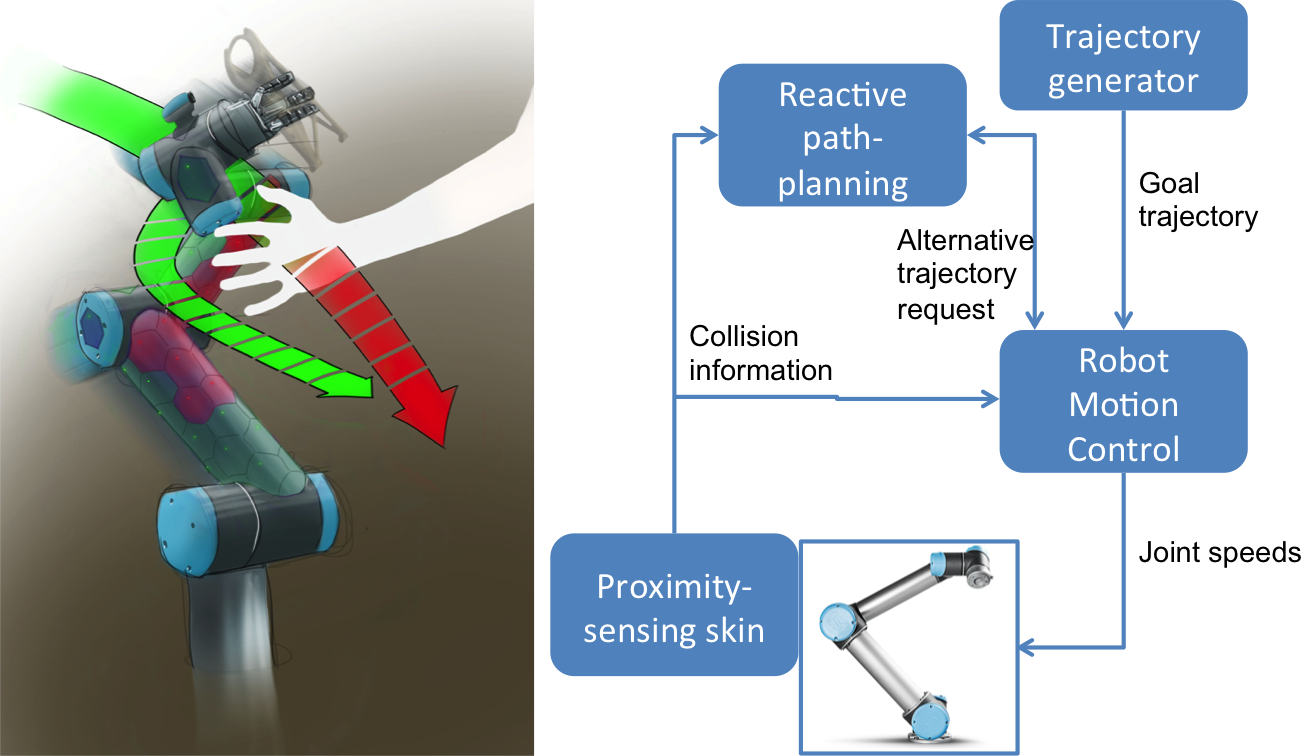
\includegraphics{doa/images/overview.png}}
\caption[]{An artist's schematization of the FiaD Dynamic obstacle avoidance
concept is illustrated on the left side. On the right, an overview of the main
components of the solution.}
\label{fig:overview}

\end{figure}

\begin{figure}[h]
\centering
\resizebox{0.8\columnwidth}{!}{\includegraphics{doa/images/sensor_unit.pdf}}
\caption[]{Robot skin developed at Institute for Cognitive Systems (ICS), TUM.}
\label{fig:RobotSkin}
\vspace{-10pt}
\end{figure}	

\subsection{Artificial Robot Skin}
The robot skin system is modularized and transduces multi-modal tactile stimuli \cite{MittendorferYC15}. The robot skin consists of hexagonally shaped PCB modules called skin cells (see Fig. \ref{fig:RobotSkin}). A group of directly connected skin cells is termed skin patch. All skin cells are identical and contain the same set of sensors. The sensors sample 9 tactile stimuli of 4 different modalities, namely vibration (3D acceleration sensor), 3 normal forces (capacitive force sensor), 2 temperatures and 1 distance (optical proximity sensor). These sensors are either off-the-shelf standard ICs or in the case of the force sensors a in-house development. A micro-controller in the back of each skin cell collects data from its sensors, filters it and creates and sends data packets, which contain the most recent values of all sensors. All the skin cells are connected to each other via stretchable flex PCBs which allows the skin to cover curved surfaces and increases its robustness. The network of skin cells is a meshed bidirectional communication network which is routed by the micro-controllers of the skin cells. A self-organized algorithm initializes all the skin cells in a skin network and constructs a bidirectional communication path between each skin cell and the network root, the tactile section unit (TSU). The TSU converts skin network packets to standard UDP Ethernet packets and vice versa. This allows for fast low latency connections between robot skin and PC (see Fig. \ref{fig:SkinCellNetworkArchitecture}).
\begin{figure}[t]
\centering
\resizebox{0.8\columnwidth}{!}{\includegraphics{doa/images/SkinCellNetwork.pdf}}\\[-15pt]
\caption[]{The skin cell network architecture and interface to the PC.}
\label{fig:SkinCellNetworkArchitecture}
\vspace{-10pt}
\end{figure}
The robot skin system also supports the auto-calibration of spatial relationships between skin cells of a skin patch covering a 3D 
surface \cite{Mittendorfer-IROS12tendorfer} such that the kinematic chain of every skin cell to the base frame can easily be determined.  

The proximity sensors used in the skin cells are infrared based sensors. The sensor emits infrared light and captures its reflections on obstacles 
in the range from 0 to 15 cm. The strength of the reflections allows the sensor to estimate the distance between the sensor and detected objects.  

\paragraph{Evaluation of Artificial Robot Skin}
\begin{figure}[h]
\centering
\resizebox{1.0\columnwidth}{!}{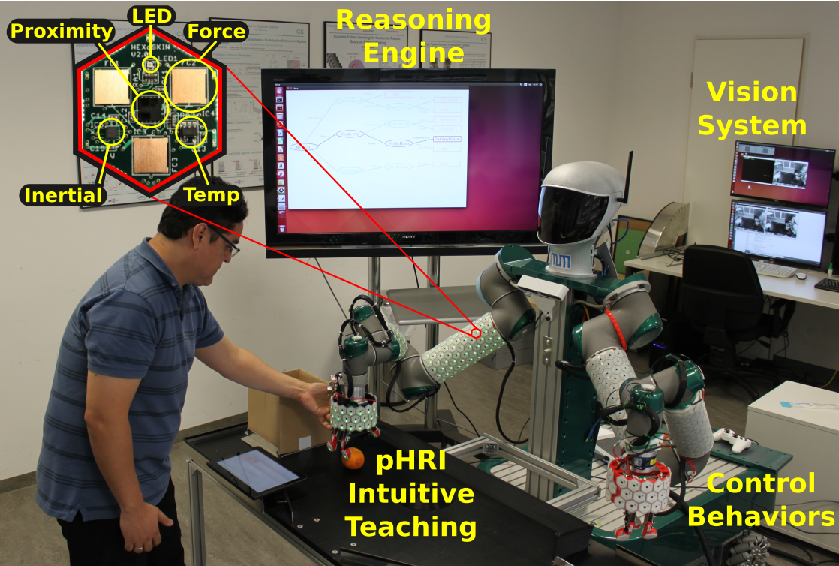
\includegraphics{doa/images/Demo.pdf}}\\[-10pt]
\caption[]{Robot TOMM. Its arms and grippers are covered with artificial robot skin. the figure depicts the robot in an industrial scenario.}
\label{fig:TommSorting}
\end{figure}

\begin{figure}[h]
\centering
\resizebox{1.0\columnwidth}{!}{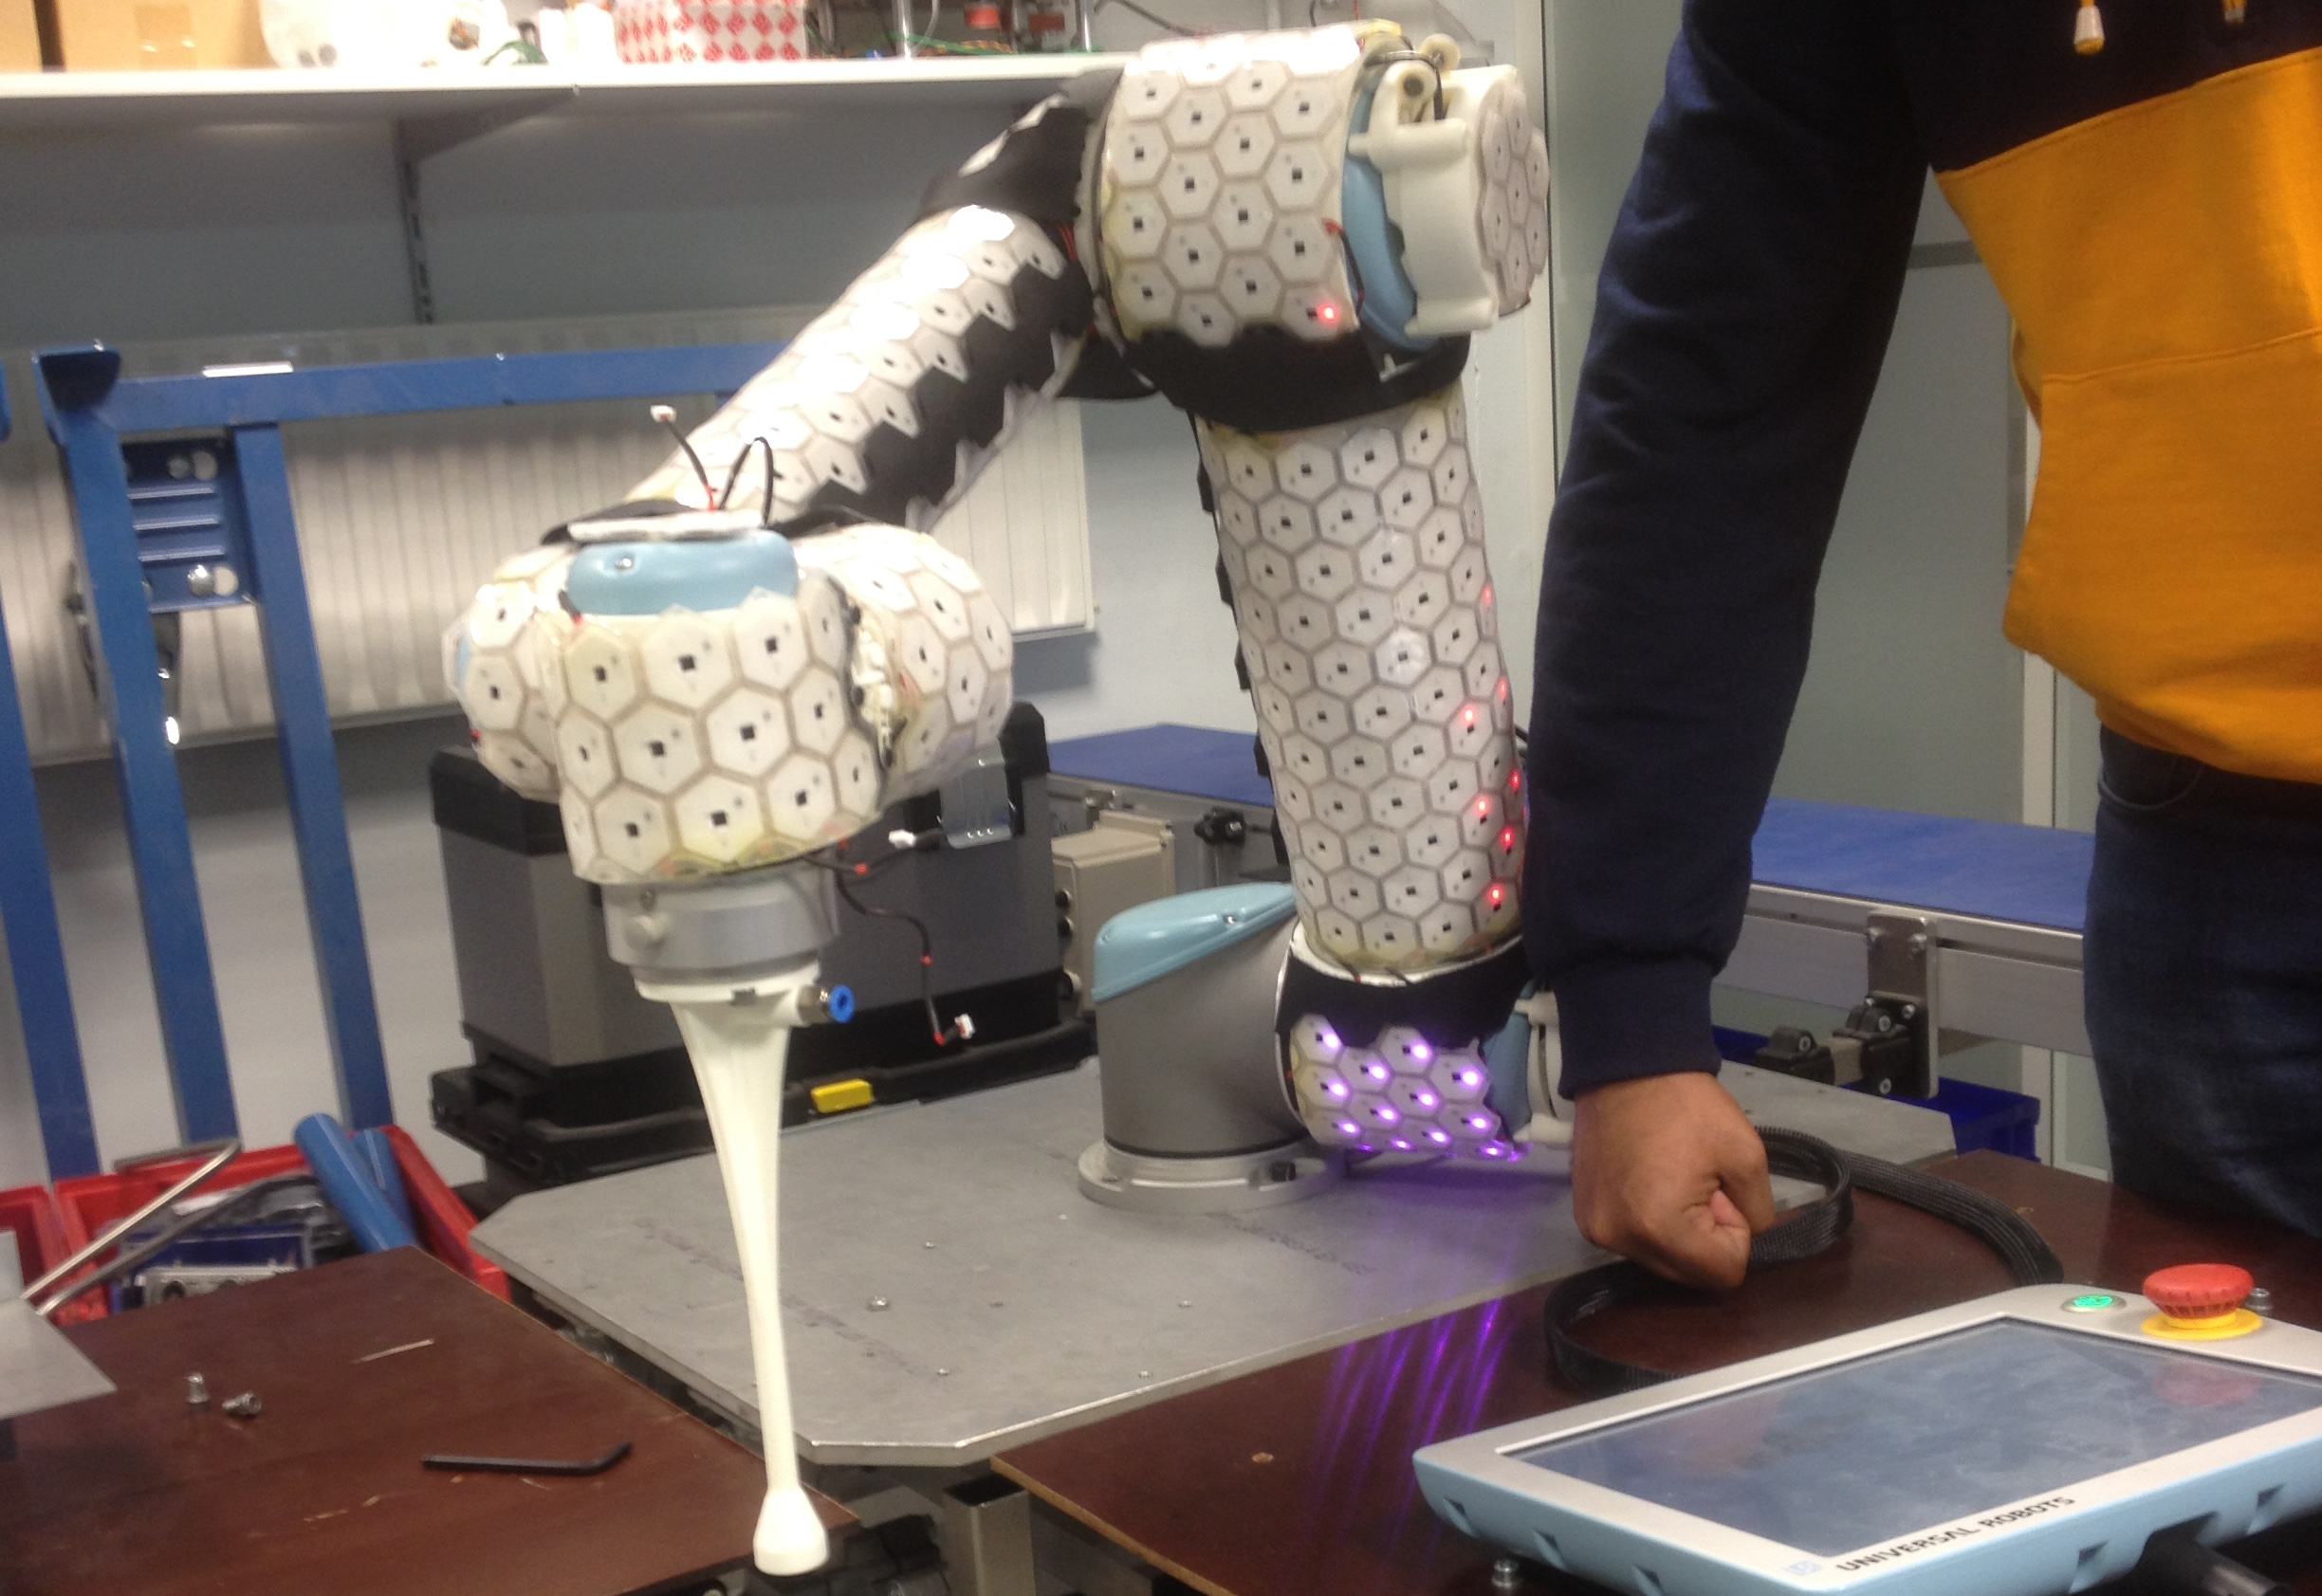
\includegraphics{doa/images/TUD_Setup.JPG}}\\[-10pt]
\caption[]{UR5 setup showing Artificial Skin Cells being activated (with red LEDs) by obstacles ($<= 6\,cm$).}
\label{fig:TUDSetup}
\end{figure}

The \textit{Artificial Robot Skin} (ARS) has been successfully deployed on the robot TOMM \cite{Dean-ICRA17} (see Fig. \ref{fig:TommSorting}). The integration of the multi-modal artificial skin signals in the control loop of the arms is demonstrated in \cite{Dean-Humanoids16} where the self-calibrating artificial skin framework is used to control the dynamic behavior of the industrial robot, e.g. producing compliance in a non-compliant robot. The advantage of these compliant behaviors is to generate safer robots, especially for physical Human-Robot Interaction. The fusion of the multi-modal signals of the artificial skin with different sensors (e.g. cameras and joint encoders) in a semantic level is demonstrated in \cite{Ramirez-Amaro-Humanoids16}. These semantic representations are used to extract general task structures which together with the obtained knowledge can improve and accelerate teaching of new tasks \cite{Dynaov-Humanoids16}. Finally, the integration of these technologies has been evaluated in an industrial scenario, where a human can kinesthetically teach the robot TOMM to sort oranges \cite{Dean-IECON16} (see Fig. \ref{fig:TommSorting}).

ARS has also been deployed successfully on another practical setup with a statically mounted Universal Robots UR5 robot (see Fig. \ref{fig:TUDSetup}). In this setup, the ARS is being used to provide proximity information related to obstacles in the immediate surroundings of the robot.


\section{Reactive Controller}
The motion control is achieved using the Stack of Tasks (SoT) controller
framework \cite{Mansard2009} which employs a hierarchical jacobian control strategy eliminating the analytical inverse kinematics computation thus making it a generic controller for all robot platforms. The controller's hierarchical nature allows the robot to handle multiple kinematic tasks simultaneously exploiting the kinematic redundancy of the robot. The controller's real time capability comes from the high computational speed of the state of the art Hierarchical Quadratic Programming (HQP) solver backing it. 


A \emph{task} basically is a control law that achieves a specific objective which can be a free space task or just an inequality constraint that narrows down the workspace of the robot. The task function formalism is very well discussed in \cite{C.Samson1991}. In the context of our work, tasks generally include robot joint posture task, collision avoidance task, joint limits task and so on. The SoT framework handles the task priorities hierarchically in the real time to ensure there are no conflicts among tasks which is used to achieve dynamic obstacle avoidance without compromising on the main goal.

For example, let us consider a pick and place application in a collaborative
environment. The primary goal for this application is to enable a robot to move
to a (set of) desired pick and place locations repetitively. The pick and place
locations can be defined as posture tasks in SoT. However, a higher priority
task considering the collaborative nature of the environment is to avoid
collisions with obstacles that could be humans, for instance. Typically such a
task is modelled as an ``Inequality'' task and an eventual feasible solution (if
one exists) is computed by the solver by exploiting the kinematic redundancy of the robot. In the jargon of motion planning and control, this behavior is similar to a \emph{local planner}.
However, it is likely that a feasible solution is not found due to the solver
converging to a local minima\footnote{This is caused by the use of task
Jacobians. For further details, please see \cite{Mansard2009}.} In such a
scenario, SoT can also be used to leverage the services of a global planner (see
Section \ref{subsec:react_path}) from the current robot state to the goal so
that an entirely new path is obtained which is free from collisions and
consequently allowing all the specified tasks to be achieved in the order of
their priorities. In Section \ref{sec:prelim_results}, we present the
experimental results of using the SoT controller on a practical setup and in
simulation. The SoT controller has also been configured to work with the ROS-control interface. In all these setups, the proximity information from
the artificial robot skin is used as an input to the collision avoidance task. In
the following part, we briefly present the global path planner software framework
that is used when the SoT controller hits a local minima.
\begin{figure}[t]
\centering
\includegraphics[scale=0.47]{doa/images/architecture_reactive_collision_1.pdf}
% \resizebox{2\columnwidth}{!}{\includegraphics{arch_tom_3}}\\
\caption[]{Dynamic collision avoidance software architecture.}
\label{fig:dca}
\end{figure}

\section{Reactive Motion Planning}
\label{subsec:react_path}
\hypersetup{colorlinks, linkcolor=blue}
The reactive path planning software framework is based on the industry grade KineoWorks\texttrademark\footnote{See
\href{http://www.plm.automation.siemens.com/en\_us/products/open/kineo/kineoworks/index.shtml}{Kineoworks}.} path planning library from Siemens in order to provide fast and reliable robot paths. This framework has also been seamlessly integrated into the ROS-ecosystem via a ROS package called \texttt{kws\_ros\_interface} which provides the planner implementations of KineoWorks as shared objects that are readily usable in ROS-based software via the \texttt{kws\_ros\_planner} ROS node.

Robot kinematic models are provided to KineoWorks in the Unified Robot Description Format (URDF) which is a ROS standard. Furthermore, KineoWorks also accepts the standard ROS representation of a \texttt{PointCloud}\footnote{See http://wiki.ros.org/pcl} for creating collision models of dynamic obstacles in the environment. The point clouds are generated in two ways. In one scenario the point clouds are generated by a standard Kinect 3D camera that is observing the immediate environment of the robot. In the other scenario, the point clouds are generated from the proximity data obtained from the Artificial Skin. Finally, the collision detection for dynamic obstacle avoidance is performed using the Kineo\texttrademark Collision Detector (KCD)\footnote{See \href{http://www.plm.automation.siemens.com/en\_us/products/open/kineo/collision-detector/index.shtml}{KCD}.}. KCD performs 3D collision detection and minimal distance analysis between triangular mesh surfaces in assembly environments. KCD has been designed specifically to minimize memory usage and take advantage of parallel processing. The complete software architecture used for the Dynamic Collision Avoidance capability is shown in Fig. \ref{fig:dca}.


\section{Stack of Tasks}

'Stack of Tasks' is a hierarchical jacobian-based task controller framework which implements the generalized inverse kinematic formalism by Hanafusa et Al. for local control of redundant systems\cite{hanafusa1981analysis}\cite{Mansard2009ik}. The framework in the earlier stages implemented the Siciliano's extension to handle multiple equality tasks\cite{siciliano1991general}. It has evolved to handle inequality constraints implementing the state of the art solver. The framework provides a structure that orders actives tasks to compute the control law without compromising on the task priority and control continuity. The framework provides a simple scripting interface to interact with controller components during the runtime and has a wrapper to communicate with the ROS world.
\subsection{State of the Art}
Since a 6-axis robot was designed at Stanford allowing a systematic way to design a robot and compute inverse kinematic solution analytically in the seventies, robots have been widely used for a variety of applications from punching cards and palletizing food items to assembly , welding in big automobile manufacturing lines and intelligent stock handling in warehouses \cite{scheinman1969design}. Safety and reliability became a significantly potential area of research since then \cite{dhillon2012robot}. These robots are usually installed in closed chambers, fixed on the ground and absolute care is taken not to make it operational when the door is open or when the co-worker is around the robot’s workspace {safetyreqs}. The safety guidelines are obviously strict as it is crucial to avoid humans in danger. But things are changing quite rapidly and we have an increased focus on human-robot collaboration with enhanced safety in the last decade \cite{Bicchi2008,dhillon2012robot} driven by creative industrial demands and high interest in flexible mobile manipulators. The safety is evaluated based on various factors influencing the human-robot collision impact such as the proximity distance, relative velocity, robot inertia and so on \cite{Kulic2006}. One of the main requirement is the robot’s capability to perceive the environment and react to it.



%    \begin{figure}[thpb]
%       \centering
%       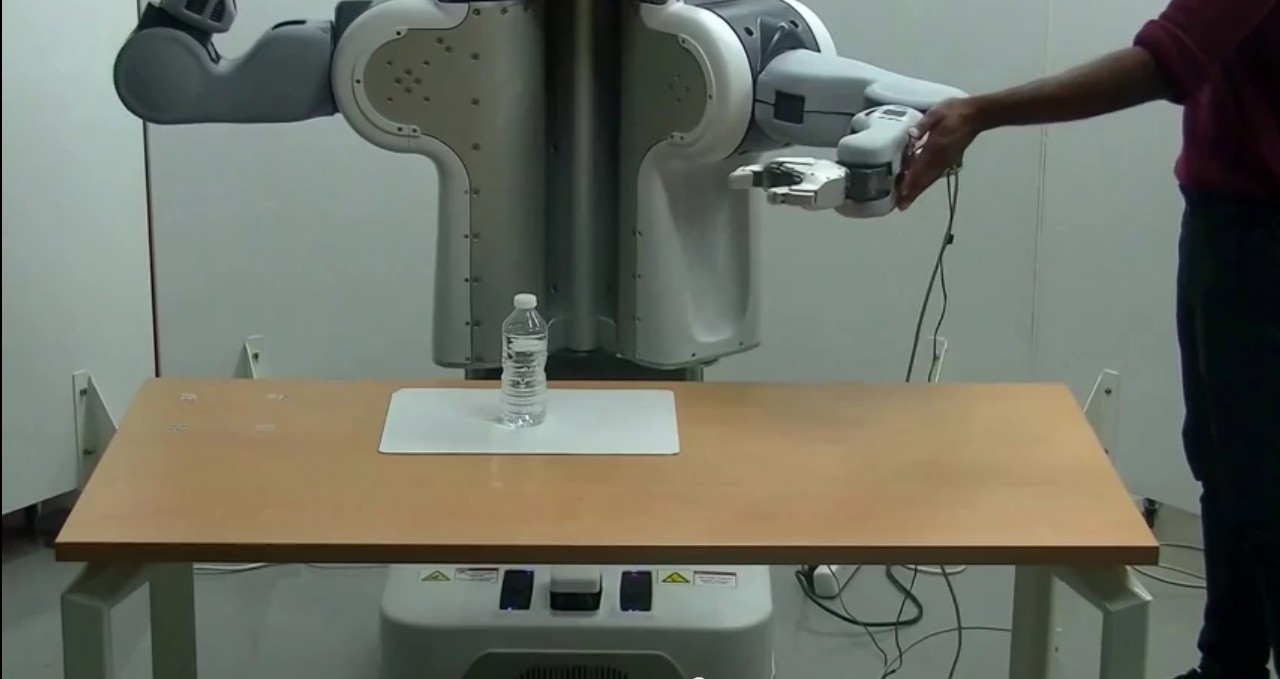
\includegraphics[scale=0.2]{doa/images/skin.eps}
%       \caption{A mobile manipulator executing a trajectory to reach a pre-grasp pose while the forearm is approached by a person with his hand. A skin sensor mounted on the forearm is used to sense any obstacle in the proximity. }
%       \label{figurelabel}
%    \end{figure}

Collision avoidance is an essential functionality in terms of safety and it is a well researched topic with various approaches  to handle different scenarios. In the earlier times, the approaches model the obstacles as static entities treating them as a planning problem to avoid collisions \cite{van2011reciprocal}. Replanning is performed based on instantaneous observations if the obstacles are dynamic. These planning based approaches limit the low level control to simple operations with controller frequencies  several times smaller than robot-environment iteration time. Constrained based approaches focus on enhancing low level control to perform complex operations by taking sensor data directly to be reactive enough with the environment \cite{khatib1986real}. The Collision avoidance can be modeled as inequality constraints or tasks in an optimization based controller. There are a variety of possible inequalities both in robot and environment in robot application scenarios. Some examples are joint limits, singularity avoidance, and object tracking in visual servoing. Constraint based robot programming were used extensively to resolve these constraints  locally but were specific to robot and the scenario involved.

Morover  redundant systems are popular due to their increased flexibility of arm and a mobile base to handle inequality constraints. The control of redundant robots is not trivial as it is not always easy to compute  analytic inverse kinematic and dynamic solutions. Task function based approach  resolves redundancy to minimize the error in task space \cite{Samson1991}. They are jacobian based techniques inverting the differential mapping that maps the control space and the error space to compute optimal controller outputs. A systematic framework for redundant system control proposed by Siciliano allowed to execute multiple tasks simultaneously with priorities {siciliano1991general}. These framework can only solve equality tasks and various strategies focuses on transforming inequality constraints to equalities\cite{Nelson95strategiesfor,chan1995weighted,mansard2009directional,raunhardt2007progressive}. These strategies are not generic enough and has priority inversion problems making them unreliable for practical use. 

A cascade approach was alternatively used to represent the inequalities and equalities systematically as a hierarchical least square program[Kanoun 2011] but suffered from computational inefficiencies. Hierarchical quadratic program (HQP) solver uses complete orthogonal decomposition (COD) instead of singular value decomposition (SVD) and an improved search algorithm which makes it more efficient than available solvers \cite{escande2014hierarchical}. Though constraint based approaches are quite an efficient way to handle collisions and a flexibile way to model them, the are merely locally optimal controllers and does not provide a systematic way to escape local minima. This necessitates the support of global path planners to find the optimal path for realizing a robot task. Combining global path planning and a reliable reactive control is an essential need for deploying robots from simple to complex scenarios.

 
\subsection{What is a Task?}
A task basically composes a control law with a specific objective which can be such as reaching a desired joint position, avoiding obstacles in the environment, a visual servoing mechanism for grasping or so on. A task is mainly defined by the error between the desired and current feature, the error jacobian and the gain. These defined tasks are pushed into 'Stack of Tasks' which computes the control law for all the task objectives in an iterative manner\cite{mansard2007task}. 

\[\textit{e(t) = x\textsuperscript{*} - x }\]

where \textit{x} refers to the current state of a feature, \textit{x\textsuperscript{*}} refers to the reference feature.

\subsection{Redundancy Formalism}
Siciliano and Slotine proposed a systematic control framework to compute controller outputs for achieving multiple tasks in redundant systems from the redundancy formalism proposed by Hanafusa et al. The idea is, tasks are solved only in the null space of the higher priority tasks to avoid conflicts with them. This means, a task at any level has no effect on the tasks in the higher level as it uses only the left degrees of freedom. 

Let $(e_{1},J_{1})$ be a primary task  which is defined by  
\begin{equation} \label{eq:tf1}
\dot{e} = J\dot{q} 
\end{equation}
 \textit{J} referring to the Jacobian of the error velocity with respect to joint velocity at the current joint state.


\begin{equation} \label{eq:tf3}
\dot{q} = J_{1}^{+}\dot{e}_{1} + Pz
\end{equation}
 Where \textit{P} is the projector on the null space of the the Jacobian J and \textit{ $z$ } is the arbitrary velocity vector which can be used as a parameter to achieve the secondary objectives. 

Let $(e_{1},J_{1})(e_{2},J_{2})...(e_{n},J_{n})$ be tasks in the stack. The redundancy formalism for two tasks can be extended to n tasks such that $e_{i}$ does not conflict with $e_{j}$ such that $j<i$. 


The recursive joint velocity is of the form
\begin{equation} \label{eq:ntasks}
  \dot{q}_{0} = 0\\
\end{equation}
\begin{equation}
  \dot{q}_{i} = \dot{q}_{i-1}+ (J_{i}P^{A}_{i-1})^{+}(\dot{e}_{i} - J_{i}\dot{q}_{i-1}), i= 1..n
\end{equation}



 where $P^{A}_{i-1}$ is the projector onto the null space of the augmented Jacobian $J_i^A = (J_1...J_i)$ and $\widetilde{J}_i = J_iP_{i-1}^A$ is the limited jacobian of the task. The joint velocity achieving all the task objectives is $\dot{q} = \dot{q}_n$. The recursive projector is computed by 
 
 \[P^A_i = P^A_{i-1} - (J_iP_{i-1}^A)^+J^A_{i-1}  \] 
 
 This systematic way of prioritizing tasks allows simultaneous execution of multiple tasks without conflicting each other.
 \subsection{Hierarchical Quadratic Programming}
Mansard et al. proposed an improved QP solver to manage multiple equality and inequality problems in a prioritized hierarchy to handle redundancies[15]. The solver handles equality tasks quite the same like in Siciliano's framework but the solver uses complete orthogonal decomposition(COD) instead of Sing for solving the least squares which is quite faster and efficient. The Hierarchical complete orthogonal decomposition(HCOD), a COD of the jacobian mapping for all the levels is used to compute primal optimum for all the constraints at once making it computationally faster. 

Kanoun et al. and De lasa et. al used a primal active search algorithm which is very expensive due to inefficient optimal active set search involving inappropriate activation and deactivation of constraints at each level along the cascade\cite{de2010feature}\cite{kanoun2011kinematic}. The HQP solver depends on a modified primal active search algorithm to make the optimal active set computation much more efficient. Lexicographic optimization formalism is introduced to maintain the active set at each iteration consistent with prior levels completely eliminating unnecessary constraint deactivations and activations. The solver is ten times faster than the classical solvers and can consider inequalities at any levels of the
hierarchy \cite{escande2014hierarchical}.
\subsection{Proximity Distance Gradient for Collision Avoidance}
The computation of the gradient of the proximity distance between the collision bodies inspired from \cite{lefebvre2005fast} is required to define inequality constraints in Stack of Tasks to avoid self-collision and with external obstacles using a proximity sensor. Let $d$ be the distance between approximated collision bodies $O_1(q)$ and $O_2(q)$. The distance between these bodies and its variation is mapped to joint actuations $q$. The distance gradient can be computed by:
\[ \frac{\partial d}{\partial q} = n_d^{'}(\frac{\partial o_1(q)}{\partial q}- \frac{\partial o_2(q)}{\partial q}) \]

where $n_d^{'}$ is the unit normal distance vector while $o_1(q)$ and $o_2(q)$ are the respective closest points. The gradient of the closest point $p$ of fixed coordinates $(\rho_1(q),\rho_2(q)....\rho_l(q))$ in the local reference frame $(e_1(q),e_2(q)...,e_l(q))$ of a collision object at joint configuration $q$ is

\[\frac{\partial p}{\partial q} =  \sum_{l=1}^{d}\rho_l(q)\frac{\partial e_l(q) }{\partial q}\]

In a 3 dimensional workspace, the expression can be written as 

\[ \frac{\partial p}{\partial q} =  (x y  z)J_\omega + J_\nu \]

where $J_\omega$ is the jacobian of the rotational degrees of freedom $J_\nu$ is the jacobian of the linear degrees of freedom. In case of the external objects, the second part of the equation can be eliminated if the object is static. 

% This work is a direct application of the HQP solver and a first attempt to combine path planning and reactive control in a jacobian based solver framework eliminating a cumbersome architecture handling the information flow between control and planning components. Stack of Tasks, a controller framework that implements the latest HQP solver is used in this work to apply the proposed methodology. The proposed methodology is tested on PR2, a mobile manipulation platform with a skin sensor mounted on the forearm of the robot to demonstrate the collision avoidance while executing a planned trajectory without compromising the final goal of the scenario. 


% The paper is organised as follows. Section \ref{sec:application} describes the solution for dynamic obstacle avoidance and Section \ref{sec:skin} discusses the proximity-sensing robot skin. In Section \ref{sec:sot} the robot motion control architecture to incorporate the collision information as safety
% constraints to dynamically adapt the trajectory is presented. Section \ref{sec:prelim_results}
% presents the preliminary results obtained in two different robot setups. Finally, in Section \ref{sec:conclusions} we present our concluding remarks and a discussion of the current work in progress.
\paragraph{Combining Path Planning and Reactive Motion Control}
The methodology is based on defining the main goal as a workspace constraint and prioritizing between safety tasks and trajectory execution task (in joint space). The figure \ref{gso} gives an intuitive idea about the stack priority order .
   \begin{figure}[thpb]
      \centering
      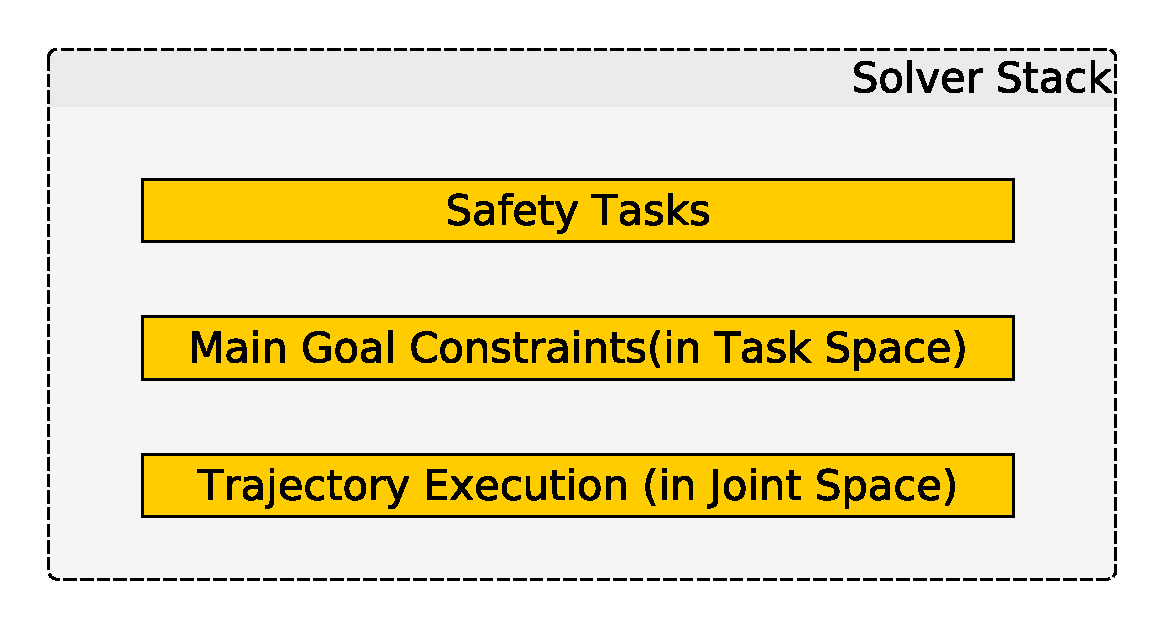
\includegraphics[scale=0.5]{doa/images/ProposedMethodology.eps}
      \caption{Generic stack order for combining planning and control. The priorities decreases from top to bottom. }
      \label{gso}
   \end{figure}

Safety tasks are obviously given higher priority in the stack for collision avoidance. Trajectory execution in Joint space occupies the least priority which leaves the controller only the left degrees of freedom from the primary task. If a base trajectory crosses an unforeseen or dynamic obstacle and if the sensors can sense it, the robot basically cannot execute the trajectory until the object is actually moved out of its way. Replanning could be activated if there is no other possibility to reach the joint trajectory goal. Even if there is a possibility to avoid the obstacle and continue executing the  trajectory, it is always not sure that the robot will end up in the desired goal in the task space. The clever trick here is in the way the main goals are defined. The main goal can be moving a base to a particular pose in the world or move the end effector to a grasping pose. Here the important thing is that the goals are something defined in the workspace though a joint trajectory is executed to achieve them. The hierarchical nature of the controller puts this main goal task in high priority and the jacobian core of the solver finds an optimal solution to follow the main goal. The next section illustrates this methodology on a simple scenario to show the potential of this method.


% \section{title}
Current collaborative robot solutions guarantee safety, but they use
obstacle detection to stop moving. Our dynamic obstacle avoidance
solution is that of using obstacle detection to respond by moving around the
obstacles while continuing to accomplish the desired tasks. Additionally, our integrated dynamic motion planning approach creates motion
plans that fulfil various task specific constraints for typical industrial
applications. For example the work cell 3D model is used to create a consistent
model of the work environment, so that collision free trajectories are flexibly 
generated for different operations. The automatic consideration of these
constraints  drastically simplifies and speeds-up the deployment of the robot.

An artist's illustration of our dynamic obstacle avoidance solution is shown
in Fig. \ref{fig:overview}. The robot motion control component generates
appropriate motion commands for the robot controller to follow the trajectories required for a given task. The proximity-sensing skin that covers the links and joints of the manipulator, produces information regarding potential collisions. This information is used by the robot motion control
module to adapt the robot motions on the fly to fulfil both constraints:
following the current trajectory (with a certain tolerance) and avoid
collisions. If the collision is unavoidable with local deformations of the
current trajectory, the robot motion control module requests a (global) re-planning,
which is performed on the fly by the reactive path-planner. The motion control
then takes the end effector to the final goal pose using the alternative
trajectory. The main functional modules of the system are discussed in the following
sections of the paper.

\begin{figure}[t]
\centering
\resizebox{0.8\columnwidth}{!}{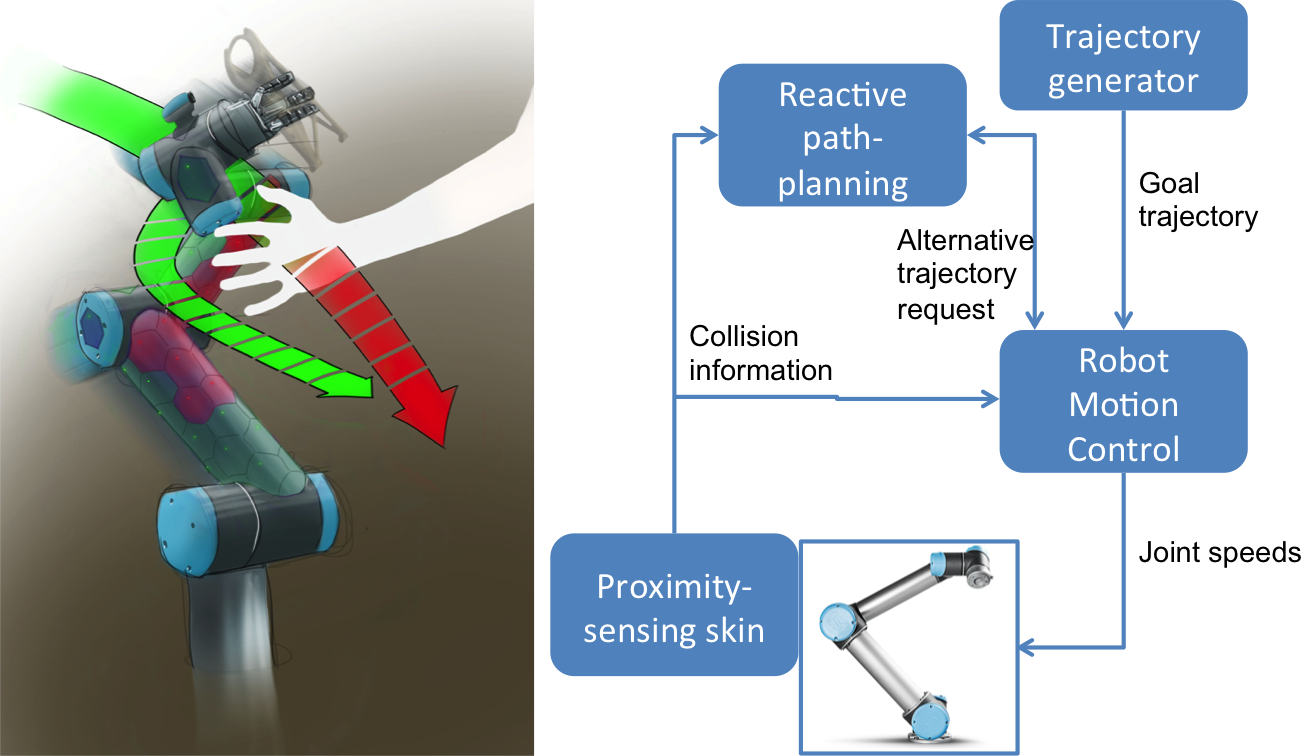
\includegraphics{doa/images/overview}}
\caption[]{An artist's schematization of the FiaD Dynamic obstacle avoidance
concept is illustrated on the left side. On the right, an overview of the main
components of the solution.}
\label{fig:overview}

\end{figure}

\begin{figure}[h]
\centering
\resizebox{0.8\columnwidth}{!}{\includegraphics{figures/sensor_unit}}
\caption[]{Robot skin developed at Institute for Cognitive Systems (ICS), TUM.}
\label{fig:RobotSkin}
\vspace{-10pt}
\end{figure}	

Our robot skin system is modularized and transduces multi-modal tactile stimuli \cite{MittendorferYC15}. 
The robot skin consists of hexagonally shaped PCB modules which we call skin cells (see Fig. \ref{fig:RobotSkin}). 
A group of directly connected skin cells is termed skin patch. All skin cells are identical and contain the same set of sensors.
The sensors sample 9 tactile stimuli of 4 different
modalities, namely vibration (3D acceleration sensor), 3 normal forces (capacitive force sensor), 2 temperatures and 1 distance
(optical proximity sensor). These sensors are either off-the-shelf standard ICs or in the case of the force sensors a in-house development.
A microcontroller in the back of each skin cell collects data from its sensors, filters it and creates and sends data packets,
which contain the most recent values of all sensors. All the skin cells are connected to each other via stretchable flex PCBs 
which allows the skin to cover curved surfaces and increases its robustness. The network of skin cells is a meshed bidirectional
communication network which is routed by the microcontrollers of the skin cells. A self-organized algorithm initializes all 
the skin cells in a skin network and constructs a bidirectional communication path between each skin cell and the network root, 
the tactile section unit (TSU). The TSU converts skin network packets to standard UDP Ethernet packets and vice versa.
This allows for fast low latency connections between robot skin and PC (see Fig. \ref{fig:SkinCellNetworkArchitecture}).
\begin{figure}[t]
\centering
\resizebox{0.8\columnwidth}{!}{\includegraphics{figures/SkinCellNetwork}}\\[-15pt]
\caption[]{The skin cell network architecture and interface to the PC.}
\label{fig:SkinCellNetworkArchitecture}
\vspace{-10pt}
\end{figure}

The robot skin system also supports the auto-calibration of spatial relationships between skin cells of a skin patch covering a 3D 
surface \cite{Mittendorfer-IROS12tendorfer} such that the kinematic chain of every skin cell to the base frame can easily be determined.  

The proximity sensors used in the skin cells are infrared based sensors. The sensor emits infrared light and captures its reflections on obstacles 
in the range from 0 to 15 cm. The strength of the reflections allows the sensor to estimate the distance between the sensor and detected objects.   

\section{Combining motion Planning and control}
There are three kind of paradigms that classifies robot's architecture\cite{asada1986robot}. The first one being the deliberative architectures work on Sense-Plan-Act strategy with environment models to represent the world. They are less reliable for reactivity and human safety because an erroneous representation of world could result in an unfortunate situation. Reactive architectures work on Sense-Act strategy which encompasses the constraint based local controllers on which we had a short look. Though they are reliable for safety, they are only locally optimal and it is impossible to operate independently. The final architecture and the one we are interested is the hybrid architecture that can combine the potential advantages of both the components to successfully realize complex scenarios without compromising safety and reliability. 

The straight forward way to combine both of them is to execute a trajectory and use reactive techniques to take care of safety. If the robot hits a local minimum or a kinematic/task singularity, re-planning mode could be activated. These reactive techniques should basically deform a planned trajectory to achieve the desired goal while taking care of the safety simultaneously. The hierarchical jacobian controller in fact does trajectory deformations which is granted for free by the solver\cite{escande2014hierarchical}. The proposed method actually exploits the hierarchical nature of the solver to perform the deformations without sacrificing the main goal. 

\section{Reactive Control Framework}
The motion control is achieved using the Stack of Tasks (SoT) controller
framework \cite{Mansard2009} which employs a hierarchical jacobian control strategy eliminating the analytical inverse kinematics computation thus making it a generic controller for all robot platforms. The controller's hierarchical nature allows the robot to handle multiple kinematic tasks simultaneously exploiting the kinematic redundancy of the robot. The controller's real time capability comes from the high computational speed of the state of the art Hierarchical Quadratic Programming (HQP) solver backing it. 


A \emph{task} basically is a control law that achieves a specific objective which can be a free space task or just an inequality constraint that narrows down the workspace of the robot. The task function formalism is very well discussed in \cite{C.Samson1991}. In the context of our work, tasks generally include robot joint posture task, collision avoidance task, joint limits task and so on. The SoT framework handles the task priorities hierarchically in the real time to ensure there are no conflicts among tasks which is used to achieve dynamic obstacle avoidance without compromising on the main goal.

For example, let us consider a pick and place application in a collaborative
environment. The primary goal for this application is to enable a robot to move
to a (set of) desired pick and place locations repetitively. The pick and place
locations can be defined as posture tasks in SoT. However, a higher priority
task considering the collaborative nature of the environment is to avoid
collisions with obstacles that could be humans, for instance. Typically such a
task is modelled as an ``Inequality'' task and an eventual feasible solution (if
one exists) is computed by the solver by exploiting the kinematic redundancy of the robot. In the jargon of motion planning and control, this behaviour is similar to a \emph{local planner}.
However, it is likely that a feasible solution is not found due to the solver
converging to a local minima\footnote{This is caused by the use of task
Jacobians. For further details, please see \cite{Mansard2009}.} In such a
scenario, SoT can also be used to leverage the services of a global planner (see
Section \ref{subsec:reactive_path}) from the current robot state to the goal so
that an entirely new path is obtained which is free from collisions and
consequently allowing all the specified tasks to be achieved in the order of
their priorities. In Section \ref{sec:prelim_results}, we present the
experimental results of using the SoT controller on a practical setup and in
simulation. The SoT controller has also been configured to work with the ROS-control interface. In all these setups, the proximity information from
the artificial robot skin is used as an input to the collision avoidance task. In
the following part, we briefly present the global path planner software framework
that is used when the SoT controller hits a local minima.



\subsection{Stack of Tasks}
'Stack of Tasks' is a hierarchical jacobian-based task controller framework which implements the generalized inverse kinematic formalism by Hanafusa et Al. for local control of redundant systems\cite{hanafusa1981analysis}\cite{Mansard2009ik}. The framework in the earlier stages implemented the Siciliano's extension to handle multiple equality tasks\cite{siciliano1991general}. It has evolved to handle inequality constraints implementing the state of the art solver. The framework provides a structure that orders actives tasks to compute the control law without compromising on the task priority and control continuity. The framework provides a simple scripting interface to interact with controller components during the runtime and has a wrapper to communicate with the ROS world.


\subsection{What is a Task?}
A task basically composes a control law with a specific objective which can be such as reaching a desired joint position, avoiding obstacles in the environment, a visual servoing mechanism for grasping or so on. A task is mainly defined by the error between the desired and current feature, the error jacobian and the gain. These defined tasks are pushed into 'Stack of Tasks' which computes the control law for all the task objectives in an iterative manner\cite{mansard2007task}. 

\[\textit{e(t) = x\textsuperscript{*} - x }\]

where \textit{x} refers to the current state of a feature, \textit{x\textsuperscript{*}} refers to the reference feature.

\subsection{Redundancy Formalism}
Siciliano and Slotine proposed a systematic control framework to compute controller outputs for achieving multiple tasks in redundant systems from the redundancy formalism proposed by Hanafusa et al. The idea is, tasks are solved only in the null space of the higher priority tasks to avoid conflicts with them. This means, a task at any level has no effect on the tasks in the higher level as it uses only the left degrees of freedom. 

Let $(e_{1},J_{1})$ be a primary task  which is defined by  
\begin{equation} \label{eq:tf1}
\dot{e} = J\dot{q} 
\end{equation}
 \textit{J} referring to the Jacobian of the error velocity with respect to joint velocity at the current joint state.


\begin{equation} \label{eq:tf3}
\dot{q} = J_{1}^{+}\dot{e}_{1} + Pz
\end{equation}
 Where \textit{P} is the projector on the null space of the the Jacobian J and \textit{ $z$ } is the arbitrary velocity vector which can be used as a parameter to achieve the secondary objectives. 

Let $(e_{1},J_{1})(e_{2},J_{2})...(e_{n},J_{n})$ be tasks in the stack. The redundancy formalism for two tasks can be extended to n tasks such that $e_{i}$ does not conflict with $e_{j}$ such that $j<i$. 


The recursive joint velocity is of the form
\begin{equation} \label{eq:ntasks}
  \dot{q}_{0} = 0\\
\end{equation}
\begin{equation}
  \dot{q}_{i} = \dot{q}_{i-1}+ (J_{i}P^{A}_{i-1})^{+}(\dot{e}_{i} - J_{i}\dot{q}_{i-1}), i= 1..n
\end{equation}



 where $P^{A}_{i-1}$ is the projector onto the null space of the augmented Jacobian $J_i^A = (J_1...J_i)$ and $\widetilde{J}_i = J_iP_{i-1}^A$ is the limited jacobian of the task. The joint velocity achieving all the task objectives is $\dot{q} = \dot{q}_n$. The recursive projector is computed by 
 
 \[P^A_i = P^A_{i-1} - (J_iP_{i-1}^A)^+J^A_{i-1}  \] 
 
 This systematic way of prioritizing tasks allows simultaneous execution of multiple tasks without conflicting each other.
 
\subsection{Hierarchical Quadratic Programming}
Mansard et al. proposed an improved QP solver to manage multiple equality and inequality problems in a prioritized hierarchy to handle redundancies[15]. The solver handles equality tasks quite the same like in Siciliano's framework but the solver uses complete orthogonal decomposition(COD) instead of Sing for solving the least squares which is quite faster and efficient. The Hierarchical complete orthogonal decomposition(HCOD), a COD of the jacobian mapping for all the levels is used to compute primal optimum for all the constraints at once making it computationally faster. 

Kanoun et al. and De lasa et. al used a primal active search algorithm which is very expensive due to inefficient optimal active set search involving inappropriate activation and deactivation of constraints at each level along the cascade\cite{de2010feature}\cite{kanoun2011kinematic}. The HQP solver depends on a modified primal active search algorithm to make the optimal active set computation much more efficient. Lexicographic optimization formalism is introduced to maintain the active set at each iteration consistent with prior levels completely eliminating unnecessary constraint deactivations and activations. The solver is ten times faster than the classical solvers and can consider inequalities at any levels of the
hierarchy \cite{escande2014hierarchical}.
\subsection{Proximity Distance Gradient for Collision Avoidance}
The computation of the gradient of the proximity distance between the collision bodies inspired from \cite{escandestrictly} is required to define inequality constraints in Stack of Tasks to avoid self-collision and with external obstacles using a proximity sensor. Let $d$ be the distance between approximated collision bodies $O_1(q)$ and $O_2(q)$. The distance between these bodies and its variation is mapped to joint actuations $q$. The distance gradient can be computed by:
\[ \frac{\partial d}{\partial q} = n_d^{'}(\frac{\partial o_1(q)}{\partial q}- \frac{\partial o_2(q)}{\partial q}) \]

where $n_d^{'}$ is the unit normal distance vector while $o_1(q)$ and $o_2(q)$ are the respective closest points. The gradient of the closest point $p$ of fixed coordinates $(\rho_1(q),\rho_2(q)....\rho_l(q))$ in the local reference frame $(e_1(q),e_2(q)...,e_l(q))$ of a collision object at joint configuration $q$ is

\[\frac{\partial p}{\partial q} =  \sum_{l=1}^{d}\rho_l(q)\frac{\partial e_l(q) }{\partial q}\]

In a 3 dimensional workspace, the expression can be written as 

\[ \frac{\partial p}{\partial q} =  (x y  z)J_\omega + J_\nu \]

where $J_\omega$ is the jacobian of the rotational degrees of freedom $J_\nu$ is the jacobian of the linear degrees of freedom. In case of the external objects, the second part of the equation can be eliminated if the object is static. 

\section{KINEO}
\hypersetup{colorlinks, linkcolor=blue}
The reactive path planning software framework is based on the industry grade KineoWorks\texttrademark\footnote{See
\href{http://www.plm.automation.siemens.com/en\_us/products/open/kineo/kineoworks/index.shtml}{Kineoworks}.} path planning library from Siemens in order to provide fast and reliable robot paths. This framework has also been seamlessly integrated into the ROS-ecosystem via a ROS package called \texttt{kws\_ros\_interface} which provides the planner implementations of KineoWorks as shared objects that are readily usable in ROS-based software via the \texttt{kws\_ros\_planner} ROS node.

Robot kinematic models are provided to KineoWorks in the Unified Robot Description Format (URDF) which is a ROS standard. Furthermore, KineoWorks also accepts the standard ROS representation of a \texttt{PointCloud}\footnote{See http://wiki.ros.org/pcl} for creating collision models of dynamic obstacles in the environment. In our work, point clouds are generated in two ways. In one scenario the point clouds are generated by a standard Kinect 3D camera that is observing the immediate environment of the robot. In the other scenario, the point clouds are generated from the proximity data obtained from the Artificial Skin. Finally, the collision detection for dynamic obstacle avoidance is performed using the Kineo\texttrademark Collision Detector (KCD)\footnote{See \href{http://www.plm.automation.siemens.com/en\_us/products/open/kineo/collision-detector/index.shtml}{KCD}.}. KCD performs 3D collision detection and minimal distance analysis between triangular mesh surfaces in assembly environments. KCD has been designed specifically to minimize memory usage and take advantage of parallel processing. The complete software architecture used in our paper for the Dynamic Collision Avoidance functionality is shown in Fig. \ref{fig:dca}.
\begin{figure}[t]
\centering
\includegraphics[scale=0.47]{architecture_reactive_collision_1}
% \resizebox{2\columnwidth}{!}{\includegraphics{arch_tom_3}}\\
\caption[]{Dynamic collision avoidance software architecture.}
\label{fig:dca}
\end{figure}

In the following sections we present the current results we have of using the different functionalities described.




\section{Method to combine Path Planning and Reactive Motion Control}
The methodology is based on defining the main goal as a workspace constraint and prioritizing between safety tasks and trajectory execution task (in joint space). The figure \ref{gso} gives an intuitive idea about the stack priority order .
   \begin{figure}[thpb]
      \centering
      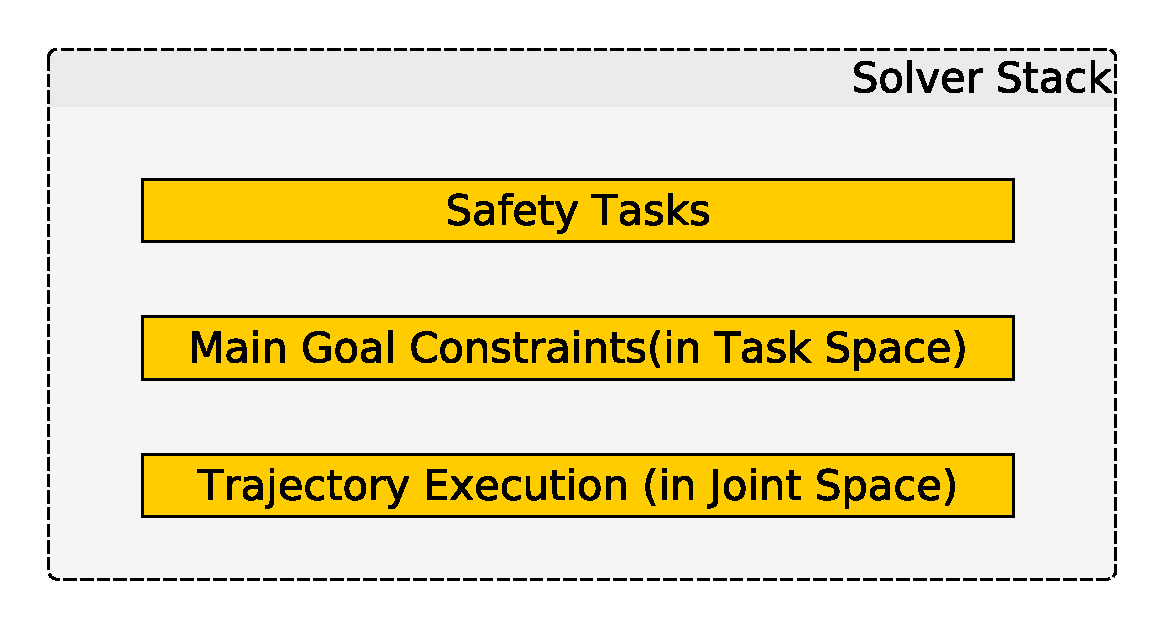
\includegraphics[scale=0.5]{doa/images/ProposedMethodology.eps}
      \caption{Generic stack order for combining planning and control. The priorities decreases from top to bottom. }
      \label{gso}
   \end{figure}

\begin{itemize}
 \item Safety tasks are obviously given higher priority in the stack for collision avoidance.
 \item Trajectory execution in Joint space occupies the least priority which leaves the controller only the left degrees of freedom from the primary task. If a base trajectory crosses an unforeseen or dynamic obstacle and if the sensors can sense it, the robot basically cannot execute the trajectory until the object is actually moved out of its way. Replanning could be activated if there is no other possibility to reach the joint trajectory goal. Even if there is a possibility to avoid the obstacle and continue executing the  trajectory, it is always not sure that the robot will end up in the desired goal in the task space. 
 
 \item The clever trick here is in the way the main goals are defined. The main goal can be moving a base to a particular pose in the world or move the end effector to a grasping pose. Here the important thing is that the goals are something defined in the workspace though a joint trajectory is executed to achieve them. The hierarchical nature of the controller puts this main goal task in high priority and the jacobian core of the solver finds an optimal solution to follow the main goal. The next section illustrates this methodology on a simple scenario to show the potential of this method.
\end{itemize}


\section{Results}
The Stack of Tasks (SoT) controller has also been deployed and tested for achieving different postures on the setup in Fig. \ref{fig:TUDSetup}. We are actively working on extending the behavior to path following and eventually integrate in accordance with the reactive collision avoidance architecture shown in Fig. \ref{fig:dca}. 


\subsection{Integrated evaluation}
\hypersetup{colorlinks, linkcolor=blue}
The integration of all the components described earlier has been evaluated on a simulation of the orange sorting setup as shown in Fig. \ref{fig:TOMMSimulation}.

\begin{figure}[h]
\centering
\resizebox{1.0\columnwidth}{!}{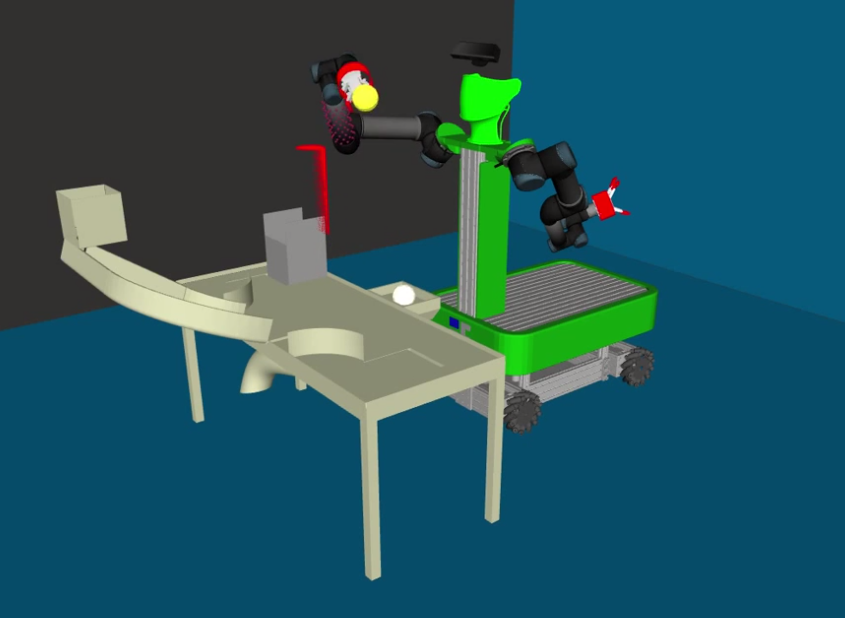
\includegraphics{doa/images/tomm_simulation.png}}\\[-10pt]
\caption[]{Orange sorting scenario in simulation.The red point cloud is a simulated obstacle.}
\label{fig:TOMMSimulation}
\end{figure}
The evaluation is done in a ROS based gazebo environment with the skin sensors simulated using the flexible collision library to project the distance between objects to sensor range measurements. 
These measurements are mapped to signals compatible in dynamic graph framework using a bridge component to allow its use in the SoT controller. The collision avoidance component computes the point 
distance and jacobian of each and every skin cell configured  essential to feed as an inequality constraint to the solver which backs the SoT controller. The planning component having the capability 
to plan with point cloud data has a Moveit python interface to query motion plan requests. The response is a set of way points which is then linearly interpolated to instantaneous joint position commands
to a path tracking task in the SoT. The SoT controller also has a python interface which makes it easy to design application scenarios.

The combined use of a reactive motion planner and a hierarchical reactive SoT controller with skin data makes it a good candidate for applying dynamical obstacle avoidance in factory environments.
A video result of the same is available \href{https://youtu.be/uLStjR7mpOI}{here}.

% \section{Experimental Illustration}
% We experimented a scenario to verify reactive trajectory execution to achieve a pre-grasp end effector configuration. The SOT framework is embedded in a ROS based real time controller running on a PR2, a mobile manipulation platform. The mobile base and the arms in this platform makes it apt for our scenarios which validates the practical advantage of the proposed methodology. A skin sensor is mounted on the forearm of the left arm . This scenario focuses on executing a simple trajectory on the left arm from an initial position (in the figure \ref{fig:init}) to reach a pregrasp position(in the figure \ref{fig:traj4}). The desired trajectory doesn't involve any movement in joints other than the left arm but they are not constrained to move as a part of the set-up. This figure \ref{ExperimentA} shows the tasks in the stack with priorities decreasing from top to bottom. 
%  The SOT controller executes a preplanned trajectory which is fed to the joint trajectory execution task in the stack. The respective end-effector pose of the trajectory at each instant is fed to an end effector pose task with a priority higher than the joint trajectory task.
%     \begin{figure}[h]
%       \centering
%       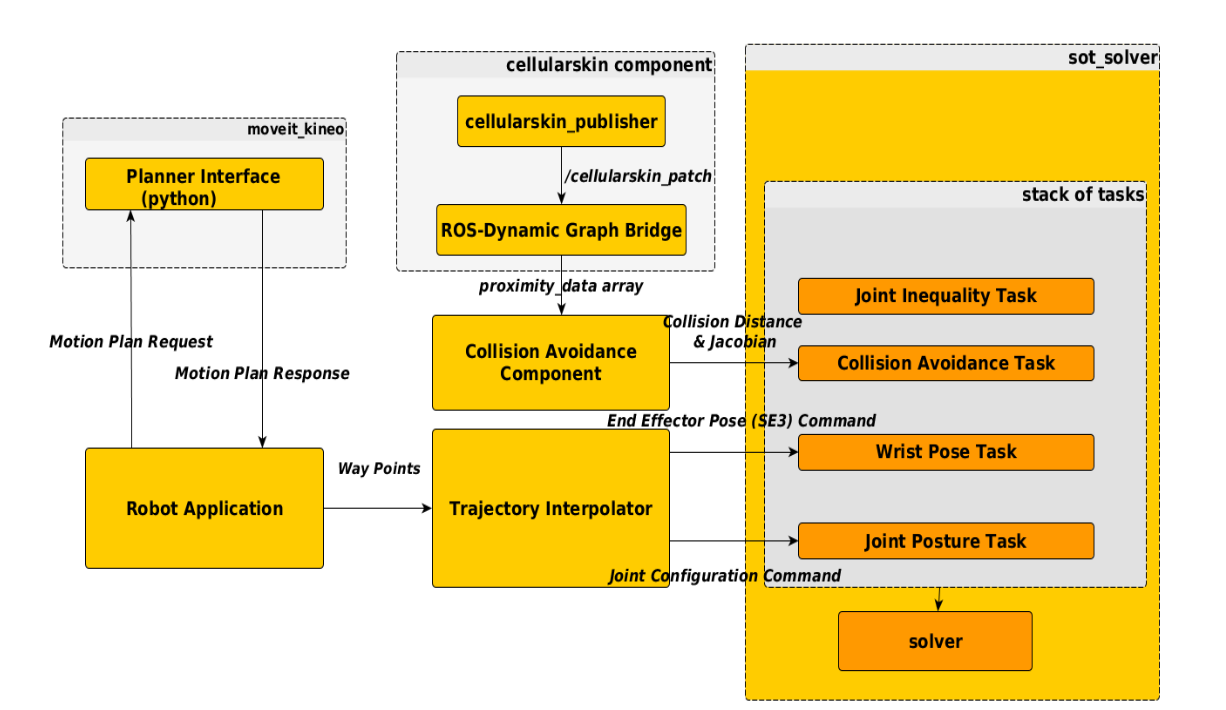
\includegraphics[scale=0.21]{doa/images/expillustration.png}
%       \caption{Robot Architecture of the Illustration Scenario}
%       \label{ExperimentA}
%    \end{figure}
 
% The planned way points are fed to a trajectory
% interpolator component which computes instantaneous joint position control
% signals to execute a joint posture task. The skin sensor component being a
% ROS based node publishes topics which are converted to signals in Dynamic
% Graph to be used by collision avoidance component necessary to compute
% information for feeding an inequality task in the solver stack. This is how
% safety and trajectory tracking are executed simultaneously. The adaptability of the controller without compromising the end goal comes
% from the pose task inserted between these tasks. The trajectory interpolator also sends a forward kinematic signal of the end effector corresponding to the joint trajectory point every instant. This allows the controller to stick with the
% plan as close as possible without violating the safety constraints and
% compromising the end goal of the scenario.



% \begin{figure}[!htb]
% \minipage{0.25\textwidth}
%   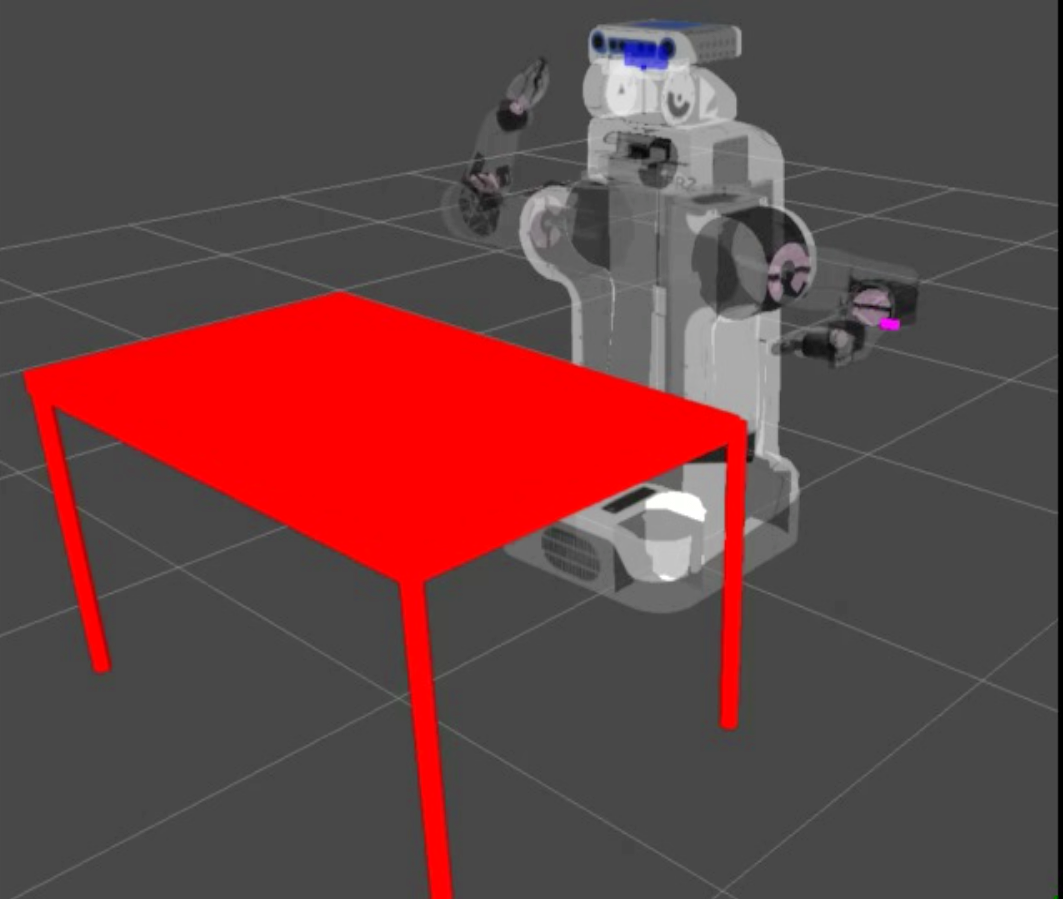
\includegraphics[width=\linewidth]{doa/images/traj1.png}
%   \caption{Initial Posture}\label{fig:init}
% \endminipage
% \minipage{0.25\textwidth}
%   \vspace{0.15\textwidth}
%   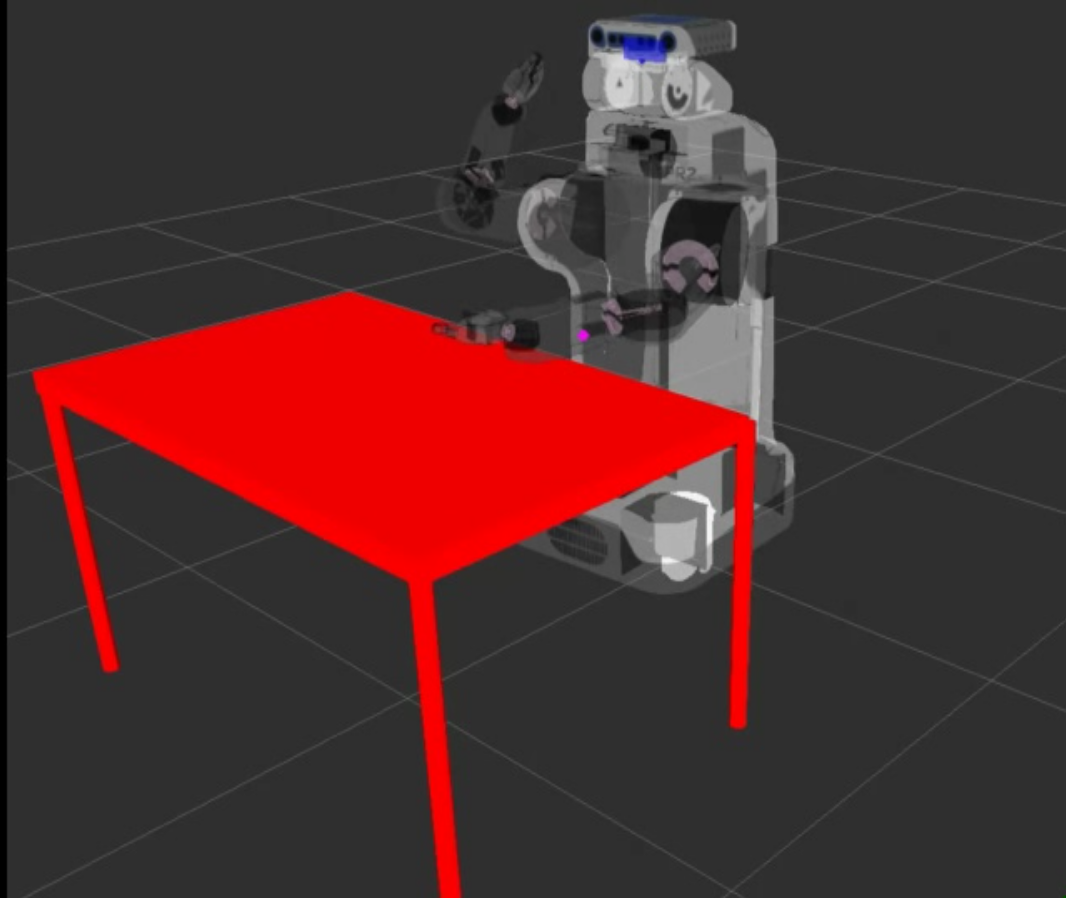
\includegraphics[width=\linewidth]{doa/images/traj4.png}
%   \caption{The robot while executing the trajectory with an actor's hand in proximity.}\label{fig:traj2}
% \endminipage\hfill
% \minipage{0.25\textwidth}%
%   \vspace{0.2\textwidth}
%   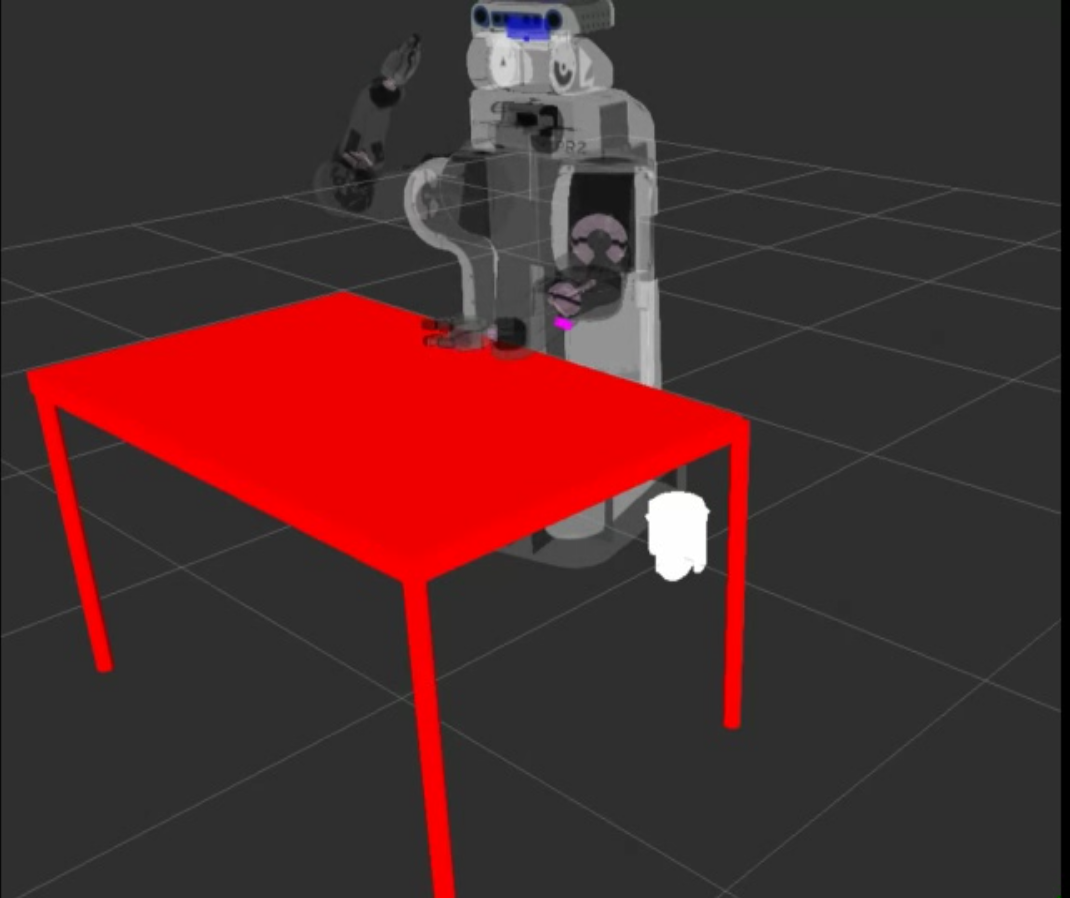
\includegraphics[width=\linewidth]{doa/images/traj8.png}
%   \caption{Base motion to avoid proximity with hand simulated yet the wrist pose is maintained.}\label{fig:traj3}
% \endminipage
% \minipage{0.25\textwidth}%
% \vspace{0.13\textwidth}
%   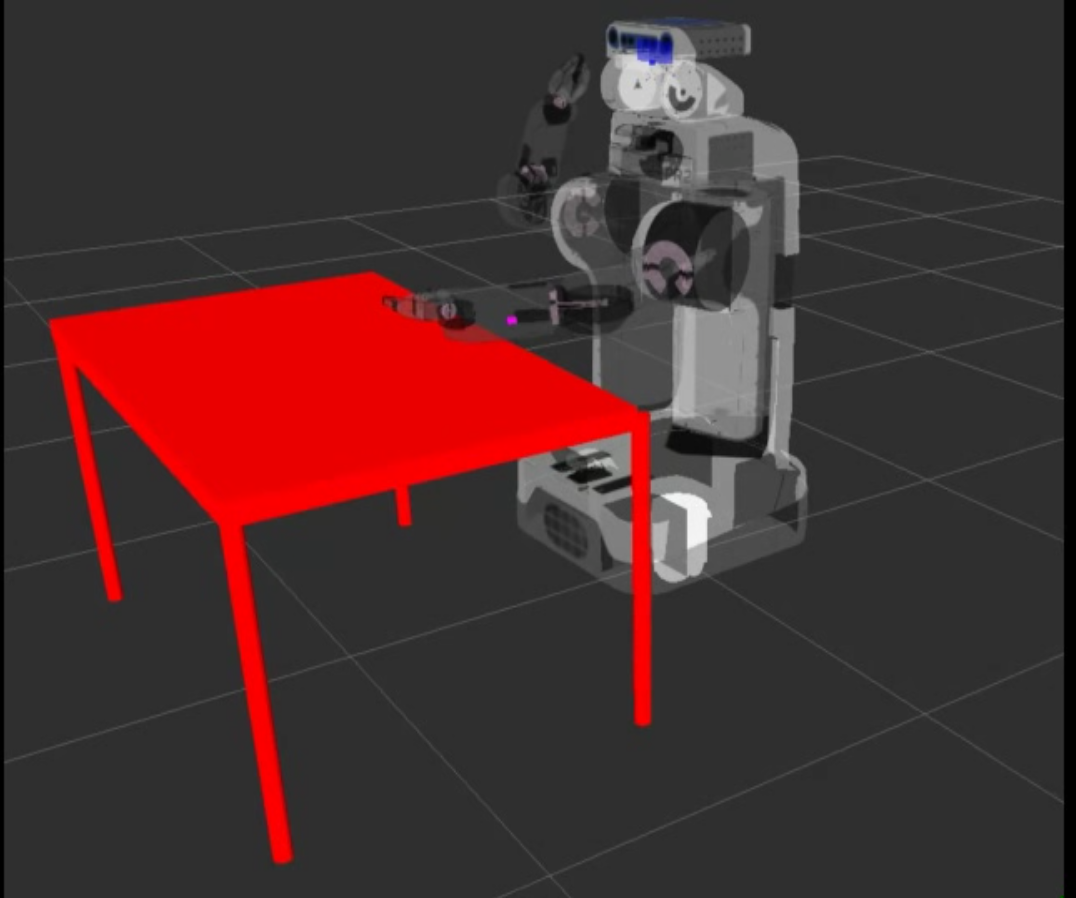
\includegraphics[width=\linewidth]{doa/images/traj11.png}
%   \caption{Final Posture after the sensor error is within the safe region.}\label{fig:traj4}
% \endminipage
% \end{figure}
   
%     \begin{figure}[!h]
%       \centering
%       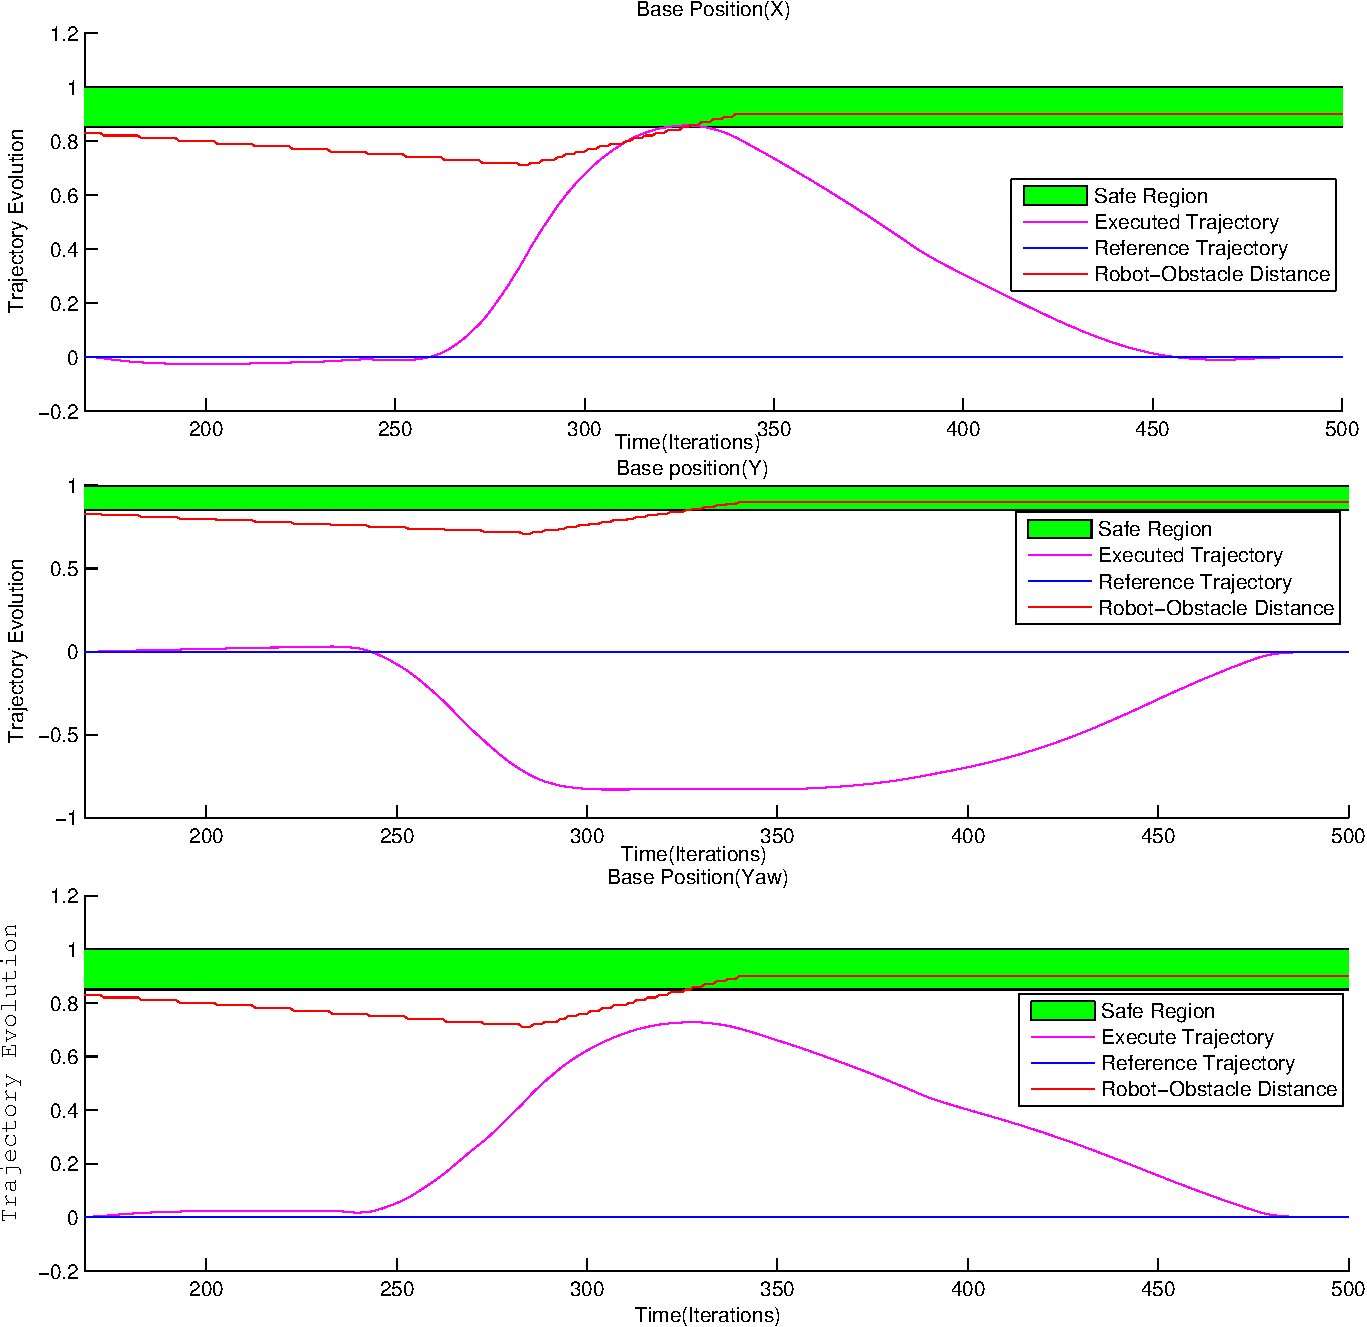
\includegraphics[scale=0.35]{doa/images/BasePlot-eps-converted-to-crop.pdf}
%       \caption{Base Motion Trajectory Evolution}
%       \label{figurebase}
%    \end{figure}  
   
%   The experiment is done in simulation and the skin sensor error is varied using a software handle. The pink colored vector on the left forearm seen in the figures \ref{fig:init} -\ref{fig:traj4} correspond to unit normal distance vector determining the direction of the robot motion in the workspace to avoid collision. The figure \ref{figurebase} shows the evolution of the base position when the sensor error oscillates between safe and unsafe regions of proximity with an obstacle. They clearly shows the base motion deviating from the reference trajectory but gets back its desired state when the error is in the safe region. The important thing is the pose of the wrist is unchanged except the yaw ( which was relaxed in the pose task to afford base motion to avoid collision while it maintains the pose)
%    \begin{figure}[!h]
%       \centering
%       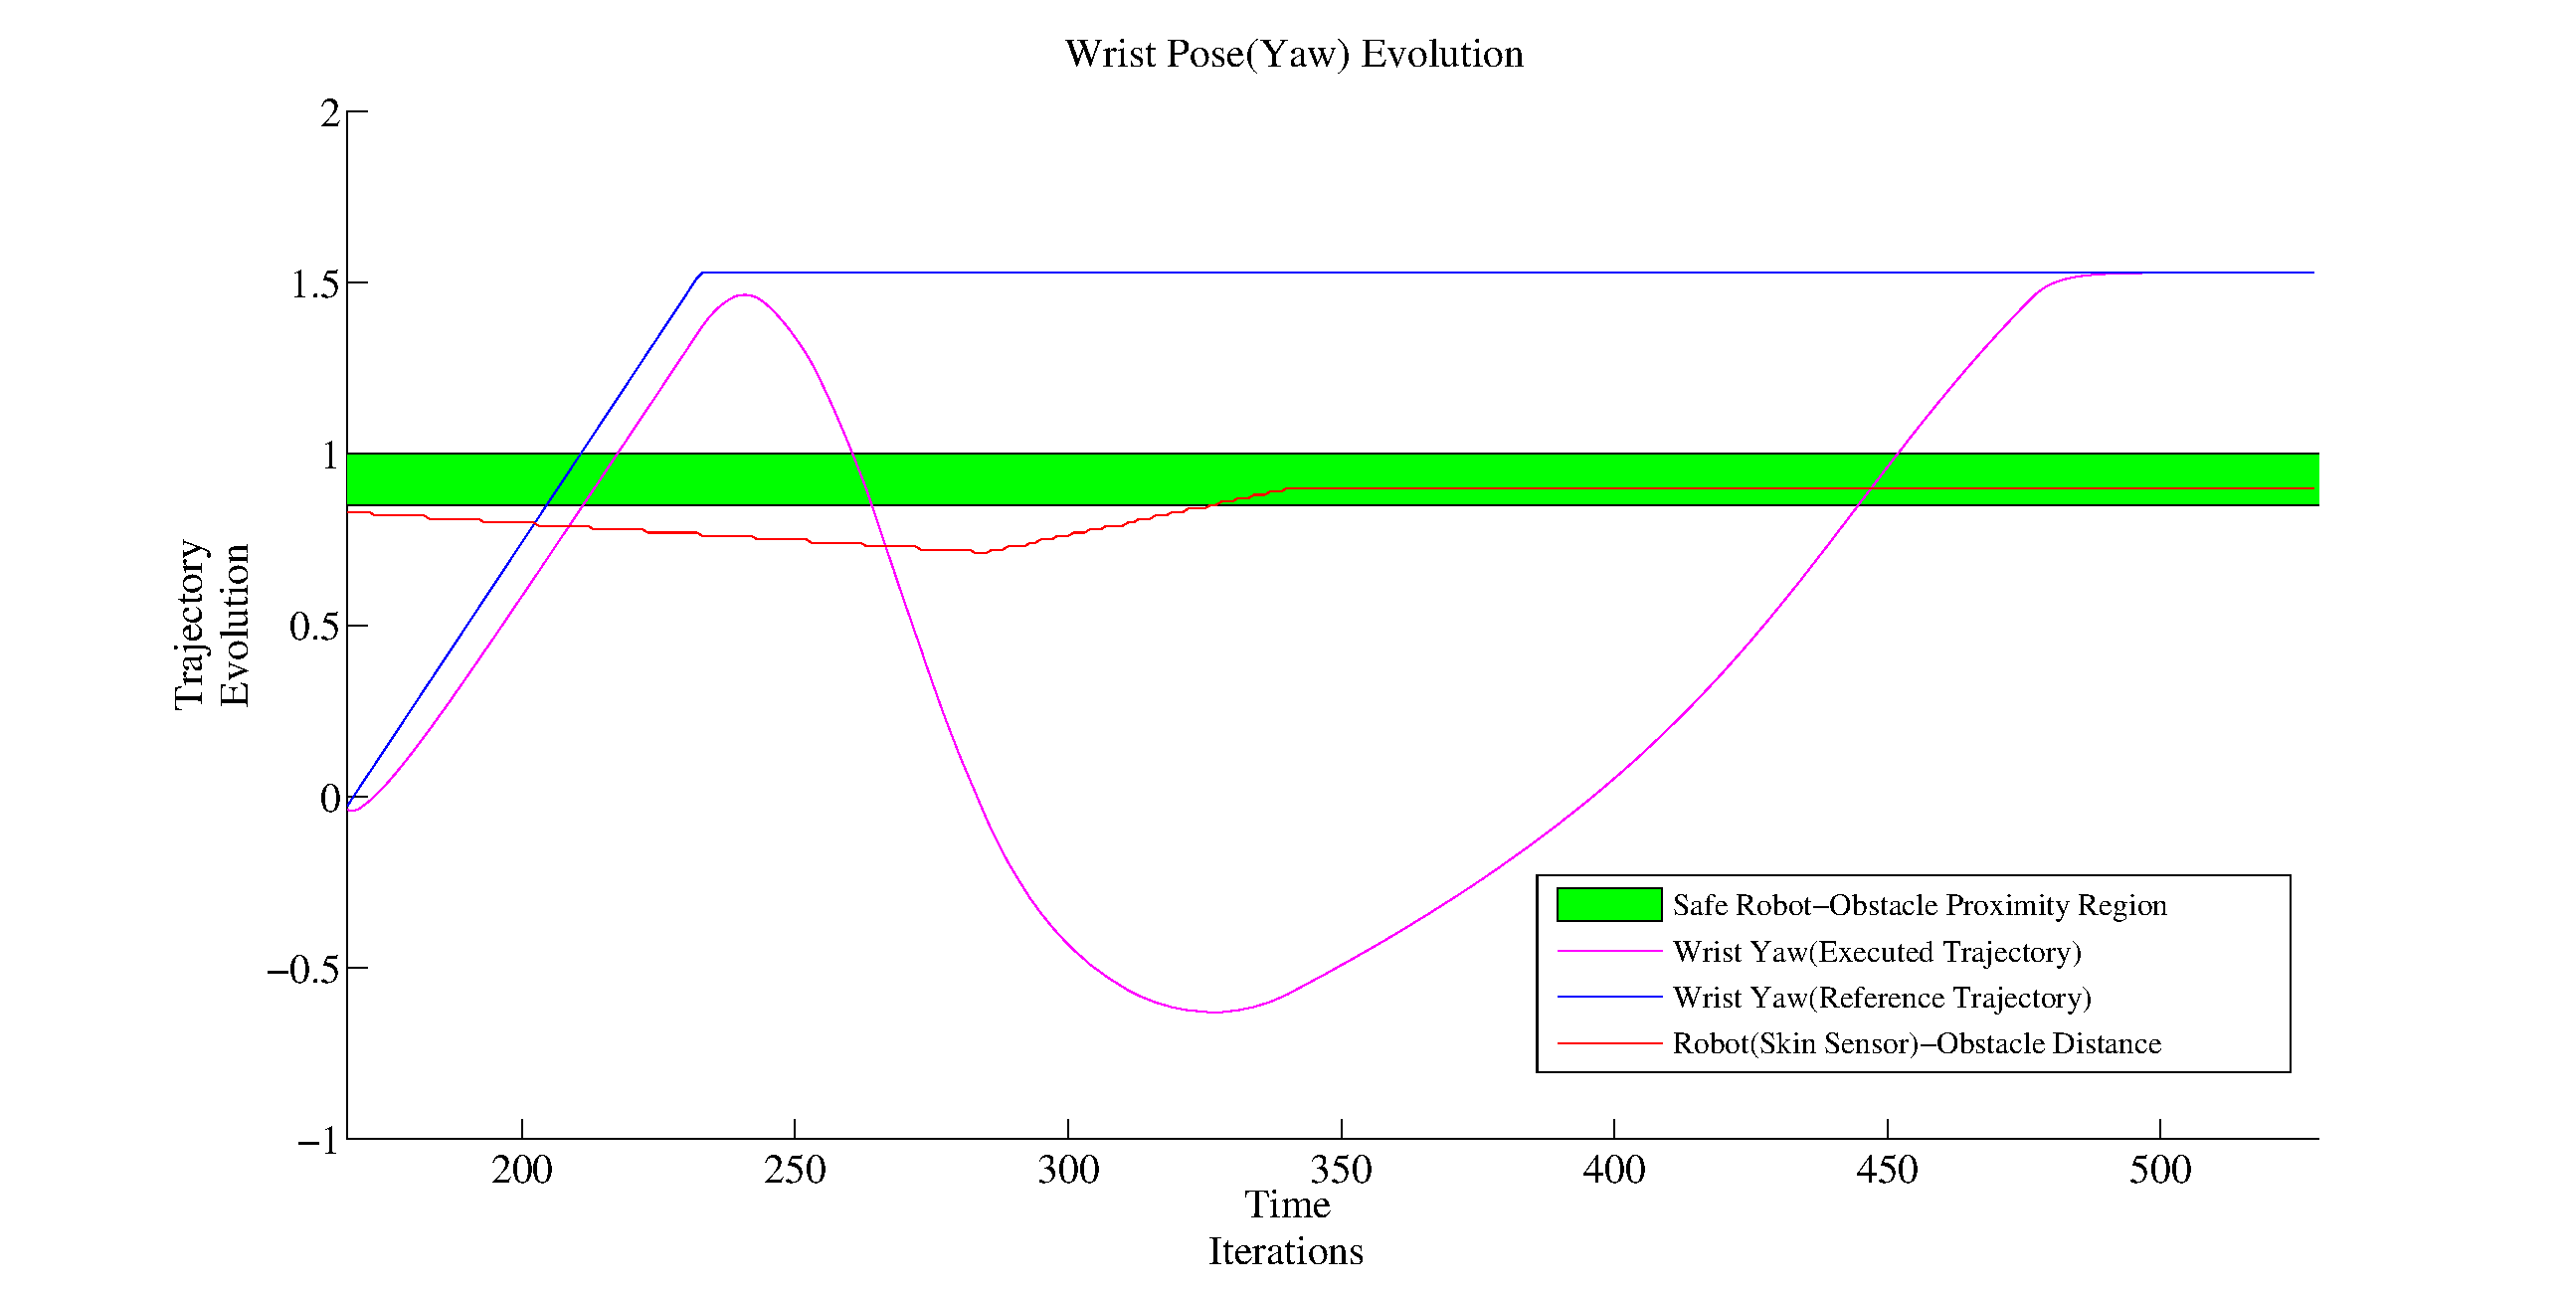
\includegraphics[scale=0.2]{doa/images/WristYawTrajectoryEvolution.eps}
%       \caption{Wrist Pose (Yaw) Evolution}
%       \label{poseYaw}
%    \end{figure}
  
% The figure \ref{poseYaw} shows the evolution of the wrist pose(yaw) of the robot which shows the connection with the base motion to compensate for the collision avoidance but yet the wrist roll and pitch in workspace doesn't change. The simple scenario could be extended to complex scenarios by figuring out the appropriate tasks corresponding to the scenario. The future work will be focused on a generic methodology to generate tasks in the stack just by specifying the scenario and feeding a trajectory.

\section{Conclusion}

This paper has presented the technologies that have been developed in the FiaD
project to augment collaborative robot manipulators with dynamic obstacle
avoidance. All these technologies: a proximity-sensing robot skin, a reactive
path planning solution and a robot motion control strategy, have been validated
in laboratory prototypes. Also, a preliminary prototype of an integrated
solution based on these technologies has been tested in simulation. With the current promising results, we are currently working on a robotic system prototype (based on the setup in Fig. \ref{fig:TUDSetup}) that will be demonstrated in a real collaborative pick-and-place application (TRL 7 \cite{TRL}) at the RoboBusiness Europe 2017 (RBE17) conference.

% work in progress%=CITE SUPPORTING EVIDENCE THAT IT WORKS=.
The integration and installation of advanced functionalities such as the dynamic
obstacle avoidance solution presented poses three main challenges from the
software point of view. The first is the integration of different components such as the skin driver, path planner and robot motion control. We address this challenge by adhering to the software development paradigm of the ROS-Industrial initiative. All the components discussed in this paper have been successfully integrated with ROS.

A second challenge is the quality assurance and robustness of the integrated robot software. This is crucial in production environments, and is specially important in collaborative applications, where safety needs to be guaranteed. For this purpose an Automated testing Framework (ATF) has been developed \cite{Weisshardt-2016} as a part of the FiaD prohect, which
allows for the systematic testing of robot software components, which includes unit
 testing, simulation-in-the-loop testing and eventually hardware-in-the-loop testing.
The tests can be automated and integrated in a centralized continuous
integration system. Preliminary test have already been conducted with the
components of the robot software system of this work, and the integrated
prototype applications will be tested with ATF.

Finally, the third challenge is the deployment of the software. One of the main barriers to transfer solutions based on robot frameworks such as ROS to industry, and specially SMEs, is how cumbersome it is
to deploy. As a part of the FiaD project, a Robot deployment toolbox has been developed \cite{Ludtke-2017}, based on ROS, which can also be integrated with ATF.
The deployment tools will also be evaluated on the RBE17 prototype.


The paper proposed a creative method to execute a trajectory robust to run-time inequality constraints without compromising on the final goal of a scenario. The method uses 'Stack of Tasks', a jacobian control framework employing the state of the art HQP solver for both equality and inequality constraints. The creativity lies on the way the hierarchical nature of the solver and flexible task definition of the framework is exploited to combine an intuitive main goal definition and reactive trajectory execution to realize a scenario successfully robustly. Experiments were done to verify the validity of the method on a PR2 robot with a skin sensor(in simulation) mounted on its forearm. Future work will focus on generalizing the method for various kind of tasks and extending the framework to systematically design tasks to be added in the controller stack specific to possible desired scenarios. The methodology has a significant potential to 
be used for a robot setup with full body skin sensors.



% DelPrete packages

\chapter{Robustness to Inertial Parameter Errors for Legged Robots Balancing on Level Ground}

% \section{Abstract}
% Model-based control  has become more and more popular in the legged robots community in the last ten years. 
% The key idea is to exploit a model of the system to compute precise motor commands that result in the desired motion.
% This allows to improve the quality of the motion tracking, while using lower gains, leading so to higher compliance.
% However, the main flaw of this approach is typically its lack of robustness to modeling errors.
% In this paper we focus on the robustness of inverse-dynamics control to errors in the inertial parameters of the robot.
% We assume these parameters to be known, but only with a certain accuracy.
% We then propose a computationally-efficient optimization-based controller that ensures the balance of the robot despite these uncertainties.
% We used the proposed controller in simulation to perform different reaching tasks with the HRP-2 humanoid robot, in the presence of various modeling errors.
% Comparisons against a standard inverse-dynamics controller through hundreds of simulations show the superiority of the proposed controller in ensuring the robot balance.


Model-based control has become more and more popular in the legged robots community in the last ten years. 
The key idea is to exploit a model of the system to compute precise motor commands that result in the desired motion.
This allows to improve the quality of the motion tracking, while using lower gains, leading so to higher compliance.
However, the main flaw of this approach is typically its lack of robustness to modeling errors. In this chapter we focus on the robustness of inverse-dynamics control to errors in the inertial parameters of the robot. We assume these parameters to be known, but only with a certain accuracy. We then propose a computationally-efficient optimization-based controller that ensures the balance of the robot despite these uncertainties. We used the proposed controller in simulation to perform different reaching tasks with the HRP-2 humanoid robot, in the presence of various modeling errors.Comparisons against a standard inverse-dynamics controller through hundreds of simulations show the superiority of the proposed controller in ensuring the robot balance.
\section{Introduction}
The problem of balancing for real legged robots is still a challenge for the robotics community.
Although our understanding of this problem has remarkably improved during the last 15 years, the robustness of the state-of-the-art control algorithms is far from satisfactory.
For instance, during the recent DARPA Robotics Challenge Finals~\cite{Pratt2015}, all legged robots have moved extremely cautiously, and, despite that, sometimes they could not avoid falling.
Another striking fact is the difference between what robots can do in simulation where they easily perform extremely dynamics tasks and what they can do in the real world where they struggle to execute slow movements in structured environments.
The gap between simulation and real world can be explained through countless unmodeled uncertainties affecting these systems, such as poor torque control, model uncertainties, sensor noises and delays.
In our recent work~\cite{DelPrete2015b} we have proposed an optimization-based controller that tries to ensure the satisfaction of the physical constraints of the robot (force friction cones, joint acceleration limits and torque limits) despite errors in the joint torque tracking. In this work we move along the same line, designing a \emph{robust} controller that can balance a legged robot despite bounded errors in its inertial parameters.




The chapter starts with a brief discussion about various control methodologies used in humanoid robots Section~\ref{sec:control_methods}. Section~\ref{sec:soa_robust} presents robustness related work in optimization based control. In Section~\ref{sec:tsid} we model the uncertainty in the inertial parameters of the robot through polytopes. Then we present the TSID controller with capture-point constraints~\cite{Ramos2014a} to ensure the balance of the robot in case of no modeling errors. Section~\ref{sec:robustness} presents an extension of the standard capture-point inequalities that is robust to errors in the inertial parameters.We first formulate the associated robust optimization problem, and then use standard robust-optimization techniques to reformulate it in a tractable form. Section~\ref{sec:tests} presents statistical results that compares in simulation the standard and the robust controller in a reaching task with the humanoid robot HRP-2. Regardless of the simulation conditions, our results empirically demonstrate the superiority of the proposed robust controller with respect to standard TSID. Finally, Section~\ref{sec:conclusions} draws the conclusions and discusses the future work.


\section{Control Methodologies in Humanoid Robotics}
\label{sec:control_methods}
Control methodologies in robotics generally define a control law that allows feasible motion generation with respect to both the robot and environmental constraints to achieve one or multiple desired tasks. There are a variety of methods to generate motion depending upon the robot, the environment and complexity of the task. The control of humanoid robots is quite specific and challenging because of the kinematic redundancy and the dynamic complexity of the system. They have a non-trivial kinematic tree structure with an essential need to stabilize the position of its center of mass(CoM) with respect to the ground at every moment while executing other tasks. In simple words, a humanoid robot cannot walk or run without knowing how to balance itself while in motion. 

Another challenging aspect to be considered here is that the dimension of task space does not equal the dimension of the actuators. Typical tasks consist in controlling the position and orientation of an end-effector (i.e. 6 dimensions), while a humanoid robot has more than 20 degrees of freedom. An inherent task-joint space mapping exists in the form of a trained nervous system in human beings but the robots need this knowledge in analytical form to make deterministic interactions with the world. Humanoid robots are under-actuated systems which means its pose cannot be controlled directly but by a consequence of commanding appropriate trajectories in joint configuration space. This section discusses the state of the art 
approaches used in generating motions.

\subsection{Motion Planning}
Motion planning in robotics refers to the process of searching discrete and feasible motion sequences to achieve a desired task usually satisfying safety constraints and optimal criteria relevant to the task. A motion planning algorithm can be used to plan motion for a variety of tasks ranging from simple arm manipulation for 6 degree of freedom (DoF) robot arms \cite{donald1987search,lozano1987simple} to advanced walking pattern generation for legged robots \cite{kajita2003biped,huang2001planning,harada2006analytical}. The basic idea is to produce continuous motion sequences that connect a start and a goal configuration of the robot while avoiding collision with the obstacles and certain criteria specific to the task. 
\paragraph{Work Space}
The \textit{Work Space}(\WS) defines the positions that a robot can and cannot reach in the 3 dimensional space of the robot. Though the robot and the obstacles are defined in the (\WS), the motion is always computed or represented in the configuration space, which usually has higher dimensions.  

\paragraph{Configuration Space}


The \textit{Configuration Space}(\CS{}) is the set of all configurations a robot can possibly attain. The \CS{} for a robot with \textit{n} degrees of freedom, is a manifold \M{} of \textit{n} dimensions with all robot configurations $q\in$\M{}. The important aspect is that the planning problem in a \WS{} of \sethree{} is transformed to a planning a point motion in its corresponding \CS{}. \CSobst{} represents the robot configurations that are self-colliding or in collision with the environment while \CSfree{} represents its complement. These subspaces allow the planning algorithm to search for a feasible path connecting the start and the end configuration avoiding collisions. 


\paragraph{Algorithms}Over the last 30 years, there has been a lot of research done in motion planning due to the variety of applications . A planning  algorithm is said to be complete if it can find a plan for all the instances of a problem when at least one exists, or report a failure if none exists. Computational complexity  is used to assess the performance of complete planning algorithms. Incomplete planners are not reliable though they are quite effective sometimes in practice. The algorithms can be categorized into \textit{deterministic} and \textit{sampling} based algorithms.
\begin{itemize}
\item \textit{Deterministic Algorithms}: These planning algorithms rely on a deterministic function to compute the path, always resulting in the same motion plan given the same planning request at any instant. Geometric approaches such as visibility graphs, cellular decomposition, Voronoi diagrams and Canny's algorithm compute the shape of \CSfree{} and its connectivity using graphs or road maps \cite{toth2004handbook,canny1988complexity} whereas Grid based approaches represents the configuration space in grids. They use search algorithms(such as $A^*$) to find a path based on the discrete number of actions within \CSfree{} region. These algorithms in general are computationally expensive for high dimensional configuration spaces. Potential field based methods \cite{barraquand1992numerical,koren1991potential} relies on artificially creaing an attractive potential field for the goal and a repulsive field to plan the instantaneous path. The approach is very efficient but it suffers from local minima. Reward based algorithms search for a path that maximizes the cumulative reward constrained by positive reward for reaching a goal and negative reward for collision with obstacles. Markov Decision Processes framework is used in most of the reward-based algorithms generating optimal path \cite{spaan2004point}. 
\item \textit{Sampling based Algorithms}: Sampling based algorithms approximate the connectivity of the feasible configurations in \CSfree{} by random sampling collision free configurations from \CS{} \cite{hudson1997v,gottschalk1996obbtree,hsu1997path}. \textit{Rapidly-exploring Random Trees}(RRT) is a quite popular algorithm which uses Voronoi bias to explore the free configuration space and grows a tree by sampling randomly at every iteration to connect the start and the goal point in \CSfree{}. In a slightly modified version referred to as \textit{Bi-directional RRT}, trees are grown from both the start and goal simultaneously to accelerate the process of the search \cite{kuffner2000rrt}. \textit{Probabilistic Roadmaps}(PRM) randomly sample from the \CS{} and connections are made with the neighbors generated by \textit{k} nearest neighbors or using a local planner \cite{karaman2011sampling}. A road map is developed by adding more configurations and connections until it is dense enough to be used for a planning problem. A path is searched or queried on the generated roadmap using Dijkstra's shortest path algorithm. There are a variety of PRM extensions to achieve better performance \cite{geraerts2004comparative}. Variations such as PRM* and RRT* for generic use cases preserve the asymptotic optimality of the tree \cite{karaman2011sampling}. Kinodynamic RRT* has been proposed for systems with controllable linear dynamics \cite{webb2013kinodynamic} and RRTs have been extended to LQR-Trees in state space \cite{tedrake2010lqr} and LQR-RRT* for linearized systems \cite{perez2012lqr}. Another extension \textit{Transition based RRT} uses stochastic optimization for computing potential states \cite{jaillet2008transition}. Sampling based algorithms deal with high dimensional configuration spaces and are probabilistically complete which means the probability that they fail to provide a solution approaches zero when more time is spent though there is no guarantee if a solution really exists or not.
\end{itemize}


Trajectory optimization is used to reduce the path length while preserving its validity. There are a variety of methods to optimize the trajectory such as greedy optimization \cite{thrun2002probabilistic}  which connects the start and the nearest node configuration that avoids obstacles in an iterative sequence until it reaches the goal configuration. 



\paragraph{Planning in Humanoid Robots}


As discussed before, Humanoid robots are under-actuated and balancing is essential to perform any other meaningful tasks. The motion planning algorithms described previously search for a collision free path considering only the geometry but do not really consider the effects of joint configurations on the whole robot itself. RRT algorithms are able to generate collision-free trajectories but do not optimize their smoothness or the associated control effort. There is a certain amount of control necessary to deterministically choose the right trajectories for tasks specific to a robot and the environment. So in humanoid robots or any polyarticulated system, inverse kinematic/dynamic or optimal control methodology can be used to generate trajectories under constraints. For instance, in humanoid robots it could be necessary to satisfy balance constraints under multiple contact while walking up the steps. In \cite{zhang2014motion}, predefined motion primitives guide the planner to generate natural trajectories.

With regard to Humanoid walking, deterministic planning approaches use a foot transition model with dynamic considerations and the trajectory smoothness during posture transitions \cite{chestnutt2005footstep,ayaz2007human} though there is no guarentee of completeness. Instead probobalistically complete methodologies like RRT can be used to search in discrete footsteps space \cite{perrin2012fast,xia2009random}. Goal-directed approaches such as in \cite{hornung2013search} ensures the path within bounded limits set by the optimal control solutions. Environment features such as contact points can also be used to guide planning \cite{bouyarmane2012dynamics,Escande2013}. There are also some approaches that decompose the problem from higher dimensions into smaller dimensions and are successively solved \cite{zhang2009motion,yoshida2008planning}. Planning is also done on constraint sub-manifolds within \CS{}. Approaches such as in \cite{bretl2006motion,hauser2010multi}, planning is done on union of sub-manifolds defined by balance constraints and leg positions for robots on uneven terrains. In \cite{berenson2011task}, they use jacobian based methods 
to add end effector pose constraints in a \textit{Constrained Bidirectional} RRT planner. In \cite{dalibard2013dynamic}, RRT is adapted within a random diffusion framework to generate statically stable trajectories. In recent times, path planning is combined with optimal contol to generate motion in cluttered environment \cite{el2013optimal}.

\subsection{Kinematic Control}
\paragraph{Basics of Robot Kinematics}
Kinematics is the study of movement of kinematic chains considering the geometry while ignoring the dynamic properties such as mass, inertia of the system and forces or torques to generate motion. The relationship between position, velocity and acceleration of the links of the system with respect to its kinematic connectivity and dimensionality is studied to control the movement of the system in joint space. The joint space of a robot with \textit{n} DoF is an \textit{n} dimensional manifold $\mathcal{Q}$ with all possible joint values. But in robotics, the pose of certain points are important for control in the task space. These point are generalized to \textit{Operational Points} \cite{Khatib1987}. The variation in an operational point x can be represented by a twist $\xi$ comprising linear and angular velocities \cite{featherstone2008rigid,Murray1994}. The kinematic control problem can be defined in four different ways:
\begin{itemize}
    \item \textit{Forward Kinematics}: Given a joint configuration $q \in \mathcal{Q}$, it involves finding the pose of an operational point $x \in SE(3)$ described by $x = f(q)$ such that $f:\mathcal{Q} \rightarrow SE(3)$. Denavit-Hartenberg(DH) parameters \cite{hartenberg1955kinematic} introduced in \cite{craig2005introduction} is quite a popular method used to represent the forward kinematics for serial manipulators though they are not suitable for closed kinematic chains and robot calibration \cite{khalil2004modeling,everett1987kinematic}. Other approaches include the \textit{Khalil-Kleinfinger} notations for closed loop robots \cite{khalil2004modeling}, \textit{Hayati-Roberts} coordinates for avoiding singularities \cite{hayati1985improving, roberts1988new}, screw theory modeling \cite{tsai1999robot}, product of exponentials(PoE) \cite{park1994computational} and methods 
    specific to humanoid robots as in \cite{kajita2005humanoid}.

    \item \textit{Forward differential kinematics}: Given a joint configuration variation $\dot{q} \in T_q(\mathcal{Q})$, it involves finding the twist of an operational point $\xi \in se(3)$ described by  $\xi = J_o(q)\dot{q}$ such that  $J_o:T_q(\mathcal{Q}) \rightarrow se(3)$ where $J_o$ is the tangent or geometric jacobian \cite{spong2006robot,Khatib1987} and $T_q(\mathcal{Q})$ is tangential to $\mathcal{Q}$ at $q$.
    \item \textit{Inverse Kinematics}: Given a pose $x \in SE(3)$ for an operational point, it involves finding the joint configuration
    $ q \in \mathcal{Q}$ described by $q = f^{-1}(x)$ such that $f^{-1}:SE(3) \rightarrow \mathcal{Q} $. The \textit{Inverse Kinematics} problem can be solved analytically for certain kinematic structures either using algebraic approaches as in \cite{paul1robot} \cite{RaghvanBoth1993inverse} or geometric approaches as in \cite{paden1985kinematics, peiper1968kinematics}.

    \item \textit{Inverse differential kinematics}: Given a joint twist $\xi \in se(3)$ for an operational point, it involves finding the 
    $\dot{q} \in T_q(\mathcal{Q})$ described by $ \dot{q} = J_o(q)^{-1}\xi$ such that $J_o^{-1}:se(3) T_q \rightarrow (\mathcal{Q})$ \cite{Chiaverini1994,Chiaverini1997,siciliano1999tricept}

\end{itemize}

\paragraph{Kinematic Redundancy}
The kinematic control involves reaching a reference point or tracking a trajectory in $SE(3)$ for one or more operational points by searching for the appropriate instantaneous joint configurations  $q(t)$. Such goals are called tasks. When the dimensions of the robot $n$ exceeds the task DoF $n_t$, the robot is said to be kinematically redundant with $n − n_t$ being the degree of redundancy with respect to task \cite{nakamura1990advanced}. Though it provides flexibility in the joint space to manage the constraints effectively, it is quite complex to handle the inverse kinematics in a multiple task scenario \cite{siciliano1991general}. Closed form solutions are not possible in redundant robots and choosing a solution that solves both the main and the complementary tasks as much as possible is essential. For instance, it is expected from a robotic arm to manipulate an object while avoiding collisions with the environmental obstacles reactively. Numerical approaches are used to solve these multi-task control problems on redundant robots.

Numerical methods formulate \textit{Inverse Kinematics} as a constrained optimization problem either globally or locally. Global methods search for an optimal path for the entire trajectory which is computational complex \cite{baillieul1990resolution}. Local methods solve them differentially computing locally optimal $dq$ for a small change $dx$ to generate the joint space trajectory $q(t)$. \textit{Resolved Motion Rate Control} in \cite{Whitney1969} finds the $dq$ by solving the system: $\dot{x} = J(q) \dot{q}$. Damped pseudo inverses \cite{nakamura1986inverse} are used to avoid singularities and inversion issues in redundant robots when the Jacobian is not a full row or column rank matrix. 

 A more generic solution solves each task by projecting onto the nullspace of the Jacobian $J$ supplying certain degrees of freedom to the specific task \cite{Liegeois1977}. There are two ways to carry out the projection systematically.

 \begin{itemize}
     \item \textit{Task Space Augmentation} uses weighting to modulate the task space by constraining the joint space\cite{sciavicco1987solving}. Task conflicts are managed by assigning weights to each task making a compromise between the goals of the tasks.  Proper tuning specific to the scenario is essential for this methodology. \textit{Extended Jacobian Matrix} helps in handling the conflict between tasks by zeroing down the projection of the cost function gradient on the null space of the Jacobian \cite{baillieul1985kinematic}.

     \item \textit{Task Prioritization} strictly prioritizes the projection hierarchically by ensuring that the lower priority task do not affect the tracking error of the higher priority task \cite{nakamura1987task}. A systematic framework for a multi-task scenarios is proposed in \cite{siciliano1991general} which algorithmically generates $\dot{q}$ to minimize the task error in a prioritized way. A solution in \cite{Baerlocher1998} is used to speed up the computation of null space projector. 
     
 \end{itemize}

\paragraph{Redundancy Resolution in Humanoid Robots}
Since humanoids and redundant robots have a tree like structure, closed form solutions are generated by treating the complete robot as a set of many kinematic chains as in \cite{ali2010closed,nunez2012explicit}. These approaches are quite complex and instantaneous inverse kinematic solvers are usually preferred. Linearizing the problem on humanoid robot, produces infinite solutions providing the possibility to perform multiple tasks. \textit{Task Space Augmentation} methods as in \cite{tevatia2000inverse} and \cite{salini2009lqp} suffer from task conflicts resulting in unsuccessful task execution whereas \textit{Task Space Prioritization} have a strict priority, computationally less expensive and are used in common. Several approaches have been developed for multiple equality constraints at the kinematic level \cite{yoshida2006task,mansard2007task,gienger2005task}. For inequality tasks, sequential quadratic programming is used to solve a cascade of tasks \cite{kanoun2009prioritizing}. A much more efficient implementation using complete orthogonal decomposition
is proposed by \cite{Escande2014} which the state of the art solver Stack of Tasks used to solve a hierarchical quadratic program. \cite{jarquin2013real} also proposes a solution for a smooth transition in control when the priorities are interchanged.  


\subsection{Dynamic Control}

\paragraph{Basics of Robotic Dynamics}
Dynamics is the study of the dynamic relationship between the motion of the kinematic chain and the generalized forces acting on the system to make movement. The relationship allows to control the robot in a dynamic level enabling a better interaction with the environment. Dynamic parameters such as length, mass, inertia of the links and the forces or torques acting on the mechanical system are considered. In a robot dynamic model, the motion is defined by joint  acceleration $\ddot{q}$ and operational point acceleration $\ddot{x}$ in the task space. Joint torques in rotational joints and joint forces are equivalent to the generalized forces considered in the relationship.

\begin{itemize}
    \item \textit{Forward Dynamics} determines the acceleration of the robot in the joint space when generalized forces are applied in the joint space
    \item \textit{Inverse Dynamics} determines the generalized forces necessary in joint space to achieve a required acceleration in the joint space.
\end{itemize}

The two main approaches to model the robot dynamics are:

\begin{itemize}
    \item \textit{Lagrange Method} is energy based with dynamic equations in closed form. \cite{uicker1969dynamic,kahn1969near,bejczy1974robot} are such approaches in the robotics domain. It has a clear separation of each component but it is very expensive  for implementing control schemes. \cite{hollerbach1980recursive} presents an efficient formulation but still \textit{Newton-Euler Method} are preferred for faster computation.
    \item \textit{Newton-Euler Method} is a generalized force based and recursive in nature. The first of its kind is presented in \cite{orin1979kinematic}. It does not clearly separate components but it is computationally cheaper. \cite{Featherstone2009} explains the most common algorithms such as the composite-rigid-body algorithm (CRBA), the articulated-body algorithm (ABA), the recursive Newton-Euler Algorithm (RNEA). 
\end{itemize}
\cite{spong1992remarks} uses an hamiltonian approach for the analysis of the robot dynamics and there exist certain numerical methods to integrate hamiltonian equations efficiently. Alternatively, \textit{Centroidal dynamics} \cite{orin2013centroidal,orin2008centroidal} models the dynamics of the CoM of the robot. Humanoid robots need to balance and the motion
usually have a large centroidal angular momentum which makes it important to 
consider the dynamics of the CoM. In contrast to the classic joint space formulation, the operational space formulation \cite{Khatib1987} defines the motion using the task space acceleration, which requires the forces to be formulated as generalized forces in the task space.

\paragraph{Dynamic Control in Humanoid Robotics}
As discussed already, classical techniques are not appropriate for humanoid robots as the control scheme has to execute coordinated motion keeping into account the interaction forces exchanged with the environment along with balance all the time. Stability criteria that constrain the CoM or the zero moment point (ZMP) within the support polygon are often enforced in the controller \cite{wieber2002stability}. A constraint on the ZMP is equivalent to a constraint on the tangential moment at the contact surfaces. The interaction of legs on the ground along with other contacts of the robot body with the environment is also necessary. The contact forces are transformed to generalized forces on the joints which can be controlled only using joint torque control. Dynamic control is quite essential in ensuring motion feasibility, agility and balance in 
humanoid robots.

The operational-space inverse-dynamics (OSID), a generic framework  establishes the whole-body control considering balance, contacts and other constraints. \cite{Khatib2004} proposes a multi-task formulation with sequential projection on  the nullspaces of the tasks at each level. Strict hierarchy allows lower priority tasks not to affect the higher priority tasks. An equivalent approach \cite{mistry2010inverse} uses orthogonal decomposition and kinematic projections to simply control when switching contact constraints and avoids the inversion of mass matrix. \cite{Righetti2011a,Righetti2011} proposes an improved version constraining the ground reaction forces with the friction boundaries. Inequality constraints can not be added in this framework which is quite necessary to implement collision avoidance, joint limits and visual servoing task. OSID's are used within optimization based methodologies to find optimal solutions. Quadratic Programming (QP) based approaches are more popular for redundant systems which allows both equality and inequality tasks. Weighting schemes are used in a QP based approach which provides robust balance \cite{collette2008robust}. \cite{Salini2011} implements a weighting focused on the task prioritization. Decoupling of the dynamics in holonomic and non-holonomic part is used in a QP to generate feasible whole body trajectories \cite{bouyarmane2012dynamics,wieber2006holonomy}. \cite{herzog2013experiments} uses active set method to implement a torque control of the lower part of the robot. OSID in a strictly prioritized QP framework is implemented in \cite{Saab2013}. 


The previous approaches focused on the robot dynamics but the angular momentum was not controlled specifically which is an important part of motion in human beings doing agile and complex motion \cite{popovic2004angular}. \cite{kajita2003resolved} proposed to control the angular momentum of the robot using the inverse of the inertia matrix. Centroidal Dynamics controls the angular momentum as in \cite{hofmann2009exploiting} focusing on gait movements and \cite{moro2013attractor} where an attractor is used to control. Also \cite{wensing2013generation} uses conic optimization techniques to control the angular momentum generating complex motions.

\subsection{Optimal Control}
Optimal Control involves finding control trajectories for a given system such that certain optimality criteria are minimized. It is a propblem of searching a set of differential equations describing the trajectory of control variables that minimizes a cost function. In Robotics, it is also called as \textit{Trajectory Optimization} or \textit{Trajectory Filtering}.

\paragraph{Background}
Optimal Control is actually an extension of a theory of \textit{Calculus of Variations} that uses optimization methodologies to find control policies. The first ever optimal control solution was proposed for the brachystochrone problem in Bernouli's work. Though there were early contributions to the theory of optimal control by Newton, Euler, Leibniz, Jacobi, Hamilton, Bolza and many others, the formalization began to take shape with the introduction of Linear Quadratic Control(LQC) problem minimizing a squared error of an expected value of a random variable x \cite{wiener1949extrapolation}. The next milestone was the birth of Dynamic Programming (DP) to solve discrete time optimal control problems which reduces the search to Hamilti-Jacobian equation. The formulation of the Pontryagin maximum principle \cite{pontryagin1987mathematical} completely formalize the problem based on the calculus of variations considering  pathwise constraints on control values of the functions. \textit{Linear Quadratic Regulator (LQR)} and the \textit{Linear Quadratic Gaussian (LQG)} are formulated to design optimal control policies in \cite{Kalman1960} which marks another important formulation in optimal control.

\textit{Model Predictive Control (MPC)} also called as Receding Horizon Control is a popular automatic control methodlogy in industries which uses the optimal control solution at each instant over a time horizon called the prediction horizon \cite{richalet1978model}. Task specific goals are specified by simple penalty functions in the optimal control which synthesizes the motion behaviour and control laws. The controller predicts the futures states under certain criteria which lets them find the control values to achieve the appropriate current state avoiding extensive exporation. \textit{Differential Dynamic Programming(DDP)} is a numerical scheme quite efficient for direct implicit optimal control generating local trajectories \cite{jacobson1968new}. A hybrid method uses constant local controllers \cite{atkeson1994using} which is improvized in \cite{atkeson2003nonparametric} using second order local models to make linear controllers.


\paragraph{Optimal Control in Humanoid Robotics}
For humanoid robot walking, the \textit{Operational Space Inverse Dynamics} or \textit{Inverse Kinematics} cannot really handle the accelerations of the CoM properly thus generating very conservative or over restricted motion. Optimal control can find 
trajectories from initial to final posture specified as one complete objective or many objectives with certain constraints. Optimal control can generate proper and powerful trajectories for CoM unlike IK or OSID. It is quite equivalent to a classical walking pattern generator in addition to the ability to incorporate whole body motion. MPC's are a quite relevant control scheme in humanoid robotics and control solutions as in \cite{kajita2003biped,herdt2010online} uses a dedicated Linearize Inverted Pendulum model to predict the future state of the system for controlling dynamic stability. Though it is quite complex and the models have to be created for every new case, optimal control is very appropriate and takes care of all the constraints at the same horizon. One problem with using optimal control in humanoid robotics is the computational time because of more DoFs and it requires a faster response when controlled in dynamic level.

In multiple task scenarios, weighted average of tasks can be used to influence the priority by choosing right weights for each task in the set \cite{dimitrov2011sparse}. It obviously introduces task conflicts if the relative difference of the weights are not significantly high. Large weights can also produce numerical errors resulting in pracitcal complexity to implement such control schemes. In \cite{del2014prioritized}, the optimal control is strictly prioritized avoding such issues. MuJoCo is a state of the art simulator that uses MPC to generate humanoid trajectories with high computational speed with respect to dynamic derivatives\cite{todorov2012mujoco}. Behaviours like getting up from the ground and avoiding disturbances were generated in this simulator \cite{tassa2012synthesis}.  The use of environment increases the controllable space to successively acheive the goals as in \cite{lengagne2013generation} generating non-coplanar contact motions. Parkour motion\cite{dellin2012framework}, kicking a ball \cite{miossec2006development} and  lifting weights \cite{arisumi2008dynamic} shows some application of optimal control in generating complex behaviours.

Variants of DDP exist with respect to optimal control in humanoid robots. Control-limited DDP allows adding inequality constraints as proposed in \cite{tassa2014control}  has been applied on a humanoid robot in simulation. Square-root DDP proposed in \cite{geoffroy2014inverse} shows that IK and OSID are special cases of optimal control without preview horizon. DDP is also used in generating sample trajectories to learn a neural network based guided policy to avoid local minima in \cite{Levine2012}. Behaviors such as walking, running, hopping and swimming are generated using this approach. Robust walking behaviours were generated using DP in \cite{whitman2013coordination} relying on multi model and learning based DP variants. Steep climbing motion is generated in \cite{Noda2014}
which uses Body Retention Load Vector to model the physical constraints. Optimal control has also been treated as an offline control problem in \cite{schultz2010modeling} optimizing energy based criteria using multiple shooting approach to generate running behaviors. Walking motions are generated without using a pattern generator but just by optimizing joint velocities, torques or ZMP constraints \cite{el2013optimal,koch2012studying}. Inverse optimal control involves learning the criteria to generate observed motions in a dynamic system. Human locomotion is studied using inverse optimal control in one such work \cite{mombaur2010human}. Also human running is studied in different terrains and distirubances in \cite{park2013inverse}


Motion planning is also combined with optimization for collision free navigation in a cluttered environment. Motion planners for high DoF systems generate trajectory in two stages: planning and optimization. There are three well known and similar techniques in this domain. CHOMP (Covariant Hamiltonian Optimization for Motion Planning) uses covariant gradient descent technique in the solver resulting in a planning algorithm completely relying on trajectory optimization \cite{zucker2013chomp}. Starting with a naive trajectory, CHOMP optimizes the dynamics of the trajectory while reacting to the obstacles in the environment. STOMP (Stochastic Trajectory Optimization for Motion Planning) is very similar except for the use of trajectory stochastic perturbations to generate trajectories without computing the jacobian \cite{kalakrishnan2011stomp}. ITOMP (Incremental Trajectory Optimization for Real-Time Replanning in Dynamic Environments) can produce suboptimal solutions because of the time constraints on the solver and the trajectory is incrementally updated online \cite{park2014high}.

High dimensionality is challenging in humanoid robotics to get optimal control working in real time. The state space gets large due to high number of DoFs and it is not easy to explore all of it apriori and generate appropriate trajectories for every cases. Current optimal control solutions are time consuming and encounters numerical problems which is sill an open issue in robotics.

\section{Robustness in Humanoid Robots}
\label{sec:soa_robust}
Even though the problem of robustness is long-standing and well-identified, it remains largely unanswered for legged robots. 
Some approaches focus exclusively on the stability of the system rather than on the feasibility of the trajectories.
For instance, adaptive control~\cite{Kelly1989} and time-delay estimation~\cite{Jin2008} try to estimate and compensate online for the major errors between nominal and real dynamic model.
Virtual model control~\cite{Pratt} does not rely on the dynamic model of the robot, which ensures robustness to errors in the inertial parameters~\cite{dietrich2013multi}. 
The main issue of these schemes is that they do not consider inequality constraints, which makes it hard to implement them on real systems, given the large number of bounds to which they are subject.

Other approaches are based on hand-tunable heuristics. For instance, a common heuristic in Task-Space Inverse Dynamics (TSID)~\cite{DelPrete2014c} which we adopt as well is to use a secondary task to keep the robot posture close to a reference one, in order to keep the movements far from the joint limits. 
Similarly, to avoid slipping/tipping, it was proposed to minimize the contact moments and the tangential contact forces in the null space of the main motion task~\cite{Righetti2010}. 
Yet another common trick during locomotion is to maintain the center of pressure close to the center of the foot~\cite{Kajita2003}.
The robotics literature is filled with these kinds of heuristics, which often are the main reason behind the successful implementations on real platforms.
However, these heuristics can not ensure feasibility in the presence of any significant uncertainty and needs ad-hoc tuning depending on the situation.

Finally, another class of works which includes this work makes use of robust optimization techniques to formulate control and planning problems.
Mordatch et al.~\cite{Mordatch2015} considered several perturbed models of a humanoid robot to plan offline a trajectory that is robust to uncertainties, reporting success rate between 80\% and 95\% on a real platform. 
Another recent work~\cite{Luo} has combined robust and time-scaling optimization to plan trajectories that are robust to bounded errors in friction coefficients and joint accelerations, whose magnitude can be estimated online through iterative learning.
Nguyen and Sreenath~\cite{Nguyen} have recently exploited control Lyapunov functions and Quadratic Programs (QPs) to ensure stability despite bounded uncertainties in the linearized system dynamics. 

Contrary to~\cite{Mordatch2015,Nguyen}, the uncertainties modeled in this work affect the parameters of the system, so they could be identified using set-membership identification techniques~\cite{Ramdani2005}.
The main contribution in this work is a novel formulation of the capture-point balance constraints, which can be included in the Task-Space Inverse Dynamics optimization problem to balance the robot despite bounded uncertainties in its inertial parameters.
Contrary to previous approaches that dealt with uncertainties to inertial parameters, our approach allows us to include inequality constraints in the problem formulation.
Thanks to this we can thus account for all the constraints to which legged robots are subject, ensuring the feasibility of the resulting trajectories.


\section{Task-Space Inverse Dynamics with Capture-Point Balance Constraints}
\label{sec:tsid}
To design a controller that is robust to errors in the inertial parameters of the robot we have first to understand how these errors affect the control action.
In this section we define the inertial parameters and we present a standard Task-Space Inverse Dynamics controller, which includes balance constraints. 
Throughout the presentation we explicitly show the dependency of the terms on the inertial parameters, while we omit the dependency on the robot configuration $q$ and velocities $v$ because they are constant values at each time step.

\subsection{Inertial Parameters}
We define the vector containing the 10 inertial parameters of link $i$ as:
\begin{equation*}
\phi_i = (m_i, m_i {}^i c_i, I_i^{xx}, I_i^{xy}, I_i^{xz}, I_i^{yy}, I_i^{yz}, I_i^{zz} ),
\end{equation*}
where $m_i \in \Rv{}$ is the mass, $c_i \in \Rv{3}$ is the CoM, $I_i \in \Rm{3}{3}$ is the 3D rotational inertia matrix.
Both $c_i$ and $I_i$ are expressed in the local reference frame of the link.
Note that $\phi_i$ does not contain directly $c_i$, but it contains only its product with $m_i$.
This is because the robot dynamics can be written in a linear form with respect to this parameterization of the inertial parameters~\cite{Traversaro2015}.

Now we can collect the inertial parameters of all the $N$ links of the robot in a single vector:
\begin{equation*}
\phi = (\phi_1, \dots, \phi_N)
\end{equation*}
We assume that each link parameters $\phi_i$ are not known exactly, but we know that they lie inside a polytope $U_i$, i.e. $\phi_i \in U_i$.
Hence also the vector $\phi$ lies inside a polytope:
$$
\phi \in U = U_1 \times \dots \times U_N
$$
Note that since a polytope can be represented by a set of linear inequalities, the constraint $\phi_i \in U_i$ can be expressed under the form $A_i \phi_i \le a_i$. Now that we defined the inertial parameters and the associated uncertainty polytopes, we can see how these uncertainties affect the controller.

\subsection{Task-Space Inverse Dynamics}
The controller that we consider in this work is an optimization-based inverse dynamics controller, which computes the desired torques taking into account the dynamcis of the robot. It has become a standard for the control of legged robots in recent years~\cite{DelPrete2014c,Herzog2016,Sentis2004,Saab2011}. Table \ref{table:simu_params} shows TSID outperforming other control frameworks.
Theortically, the kinematics and dynamics are decoupled. Kinematic level task prioritization is done first to compute acceleration and the torques are calculated to achieve the computed accelerations. 

\begin{table}[h] 
\caption{Comparison of Control Frameworks\cite{DelPrete2014c}}
\centering 
\begin{tabular}{|p{3.5cm} | p{1.2cm} p{1.2cm} p{1.2cm} p{1.2cm} p{1.4cm} p{1.1cm}|}
\hline 
	Framework		& Optimal & Efficient & Force& Under & Inequality & Output \\ 
 	& & & Control & actuated& &  \\ \rowcolor[gray]{.9}   
\hline 
	TSID\cite{DelPrete2014c}& $\times$ & $\times$ & $\times$ & $\times$ & & $\tau$ \\
	UF\cite{Peters2007}		&  & $\times$ & $\times$ &  & & $\tau$ \\  \rowcolor[gray]{.9}
	WBCF\cite{Sentis2005}	& $\times$ &  & $\times$ & $(\times)$ &  & $\tau$\\ 
	\cite{Mistry2011}		&  & & $\times$ & $\times$ & & $\tau$ \\ \rowcolor[gray]{.9}
	SoT\cite{Saab2011}		& $\times$ &  & $\times$ & $\times$ & $\times$& $\tau$ \\  
	\cite{DeLasa2009}		& $\times$ & &$\times$& $\times$ &  & $\tau$ \\  \rowcolor[gray]{.9}
	\cite{Jeong2009}		& $\times$ & $\times$ &  &  & & $\tau/\ddot{q}$ \\      
	\cite{nakamura1987task}		& & $\times$ &  &  & & $\dot{q}/\ddot{q}$ \\ \rowcolor[gray]{.9}
    	\cite{Chiaverini1997}		& & $\times$ &  &  & & $\dot{q}$ \\ 
	\cite{siciliano1991general}	& $\times$ & $\times$ &  &  & & $\dot{q}$ \\  \rowcolor[gray]{.9}

	\cite{Baerlocher1998}		& $\times$ & $\times$ &  &  & & $\dot{q}$ \\  
	\cite{Smits2008}		& $\times$ & $\times$ &  &  & $\times$& $\dot{q}$ \\   \rowcolor[gray]{.9}        
%	$K_p^{reach}$ 	& Reaching proportional gain 	& $20-80$ \\ \rowcolor[gray]{.9}
%	$K_p^{post}$ 	& Posture proportional gain 	& $20$ \\
[0.5ex] \hline 
\end{tabular} 
\label{table:simu_params} %\bigskip
\end{table}




% \explainmore{The generic method proposed in this thesis is based on the inverse-dynamics model of the robot considering contact constraints and a set of tasks specified with a given priority. The resolution for each task is posed as a minimization problem, subject to several constraints that ensure dynamic feasibility, and uses a hierarchical scheme based on hierarchized QPs. Since the motion is generated using several prioritized tasks, and the dynamic model of the robot is taken into account, the term Dynamic Stack of Tasks (SoT) is sometimes used to refer to the framework. With respect to other operational-space inversedynamics (OSID) approaches, the advantages of the proposed method are the capability to handle both equality and inequality constraints at any level of the hierarchy, the fast computation time that allows it execution in real-time, and the direct feasibility of the generated motion, which does not need any further processing or validation before being executed on the robot.}


Various formulations of the TSID optimization problem exist and are often equivalent or similar~\cite{DelPrete2014c}.
We write it here as an optimization problem of the base and joint accelerations $\dot{v} \in \Rv{n+6}$, the contact forces \mbox{$f\in \Rv{k}$}, and the joint torques $\tau \in \Rv{n}$~\cite{Saab2013}:
\begin{subequations} 
\label{eq:TSID}
\begin{align}
\minimize_{y=(\dot{v}, f, \tau)} \quad &|| A y - a||^2 \nonumber\\
\st \quad & \mat{M(\phi) & -J_c^\TS & -S^\TS \\ J_c & 0 & 0} \mat{\dot{v} \\ f \\ \tau} = \mat{- h(\phi) \\ -\dot{J}_c v} \nonumber\\
& | \tau | \le \tau^{max} \label{eq:TSID_torque_lim}\\
& \dot{v}^{min} \le \dot{v} \le \dot{v}^{max} \label{eq:TSID_acc_lim}\\
& f \in \mathcal{K} \label{eq:TSID_force_lim}
\end{align} 
\end{subequations}
where \mbox{$J_c \in \Rm{k}{(n+6)}$} is the constraint Jacobian, $M \in \Rm{(n+6)}{(n+6)}$ is the mass matrix, $h \in \Rv{n+6}$ contains the bias forces, $S\in \Rm{n}{(n+6)}$ is the selection matrix, $\tau^{max} \in \Rv{n}$ are the maximum joint torques, $\dot{v}^{min/max} \in \Rv{n+6}$ are the acceleration bounds\footnote{The bounds of the joint positions and velocities are typically converted into joint-acceleration bounds~\cite{Padois2010}}, and $\mathcal{K}$ is the force friction cone (which is typically linearized).
The cost function represents the error of the task, which is typically an affine function of $\dot{v}$ (i.e. a task-space acceleration):
\begin{equation*} \begin{aligned}
\underbrace{\mat{J_{task} & 0 & 0}}_A y - \underbrace{(\ddot{x}_{task}^{des} - \dot{J}_{task} v)}_a = \ddot{x}_{task} - \ddot{x}_{task}^{des}
\end{aligned} \end{equation*}
The task may be to track a predefined trajectory of a link, of the CoM of the robot, or to regulate the robot angular momentum.

\subsection{Capture Point}
Regardless of the task they are performing, legged robots must take care of balancing (i.e. avoiding to fall) at the same time.
Balancing is fundamental for legged robots and it has been extensively studied~\cite{Collette2008,Morisawa2012,Goswami2004,Hyon2006,Sherikov}.
This problem is particularly well understood for robots in contact with a flat terrain only.
In this case, the dynamics of the robot CoM $c$ is well approximated by a linear inverted pendulum.
In this model the robot is approximated as a point mass (maintained at a constant height) supported by a variable-length leg link~\cite{Pratt2006}.
The resulting dynamics is:
\begin{equation*}
\ddot{c}^{xy}(\phi) = \omega(\phi)^2 (c^{xy}(\phi) - u),
\end{equation*}
where $u \in \Rv{2}$ is the ZMP, which is equivalent to the center of pressure~\cite{Wieber2002}, and \mbox{$\omega(\phi) = \sqrt{\frac{g}{c^z(\phi)}}$}.
The same dynamics can also be obtained from the real dynamics of the robot CoM, by assuming that $\dot{c}^z=0$ and the rate of change of the robot angular momentum is null~\cite{Wieber}.
Using this linear dynamics we can compute the point on the ground where the robot can put its ZMP to in order to stop its CoM:
\begin{equation*}
\xi(\phi) = c^{xy}(\phi) + \frac{\dot{c}^{xy}(\phi)}{\omega(\phi)}
\end{equation*}
This point is known as the capture point~\cite{Pratt2006}, the divergent component of motion or the extrapolated CoM ~\cite{Wieber}.

\subsection{Capture-Point Balance Constraints}
Originally, the capture point was used to decide where to make the robot step in order to recover from a push~\cite{Pratt2006}.
More recently, Ramos et al.~\cite{Ramos2014a} proposed use it to ensure the balance of the robot.
The key idea is that, as long as the capture point remains inside the convex hull of the contact points (i.e. the so-called \emph{support polygon} $\mathcal{S}$), the robot can balance without taking a step. 
To ensure the balance of the robot we can then add to \eqref{eq:TSID} another set of inequalities to constrain the capture point to remain inside the support polygone:
$$
B (\xi(\phi) + \dt \dot{\xi}(\phi))  \le b,
$$
where $\dot{\xi}(\phi) \in \Rv{2}$ is the time derivative of the capture point, and the matrix $B$ and the vector $b$ define the support polygon (i.e. $B x \le b \Longleftrightarrow x \in \mathcal{S}$).
By expressing $\xi$ and its derivative as functions of $c^{xy}$ and its derivatives we get:
\begin{align*}
B \left ( c^{xy}(\phi) + \frac{\dot{c}^{xy}(\phi)}{\omega(\phi)} + \dt \left( \dot{c}^{xy}(\phi) + \frac{\ddot{c}^{xy}(\phi)}{\omega(\phi)} \right) \right)  \le b \\
B \left ( c^{xy}(\phi) + \alpha(\phi) \dot{c}^{xy}(\phi) + \frac{\dt}{\omega(\phi)} \ddot{c}^{xy}(\phi) \right)  \le b,
\end{align*}
where $\alpha(\phi) = \dt + \omega(\phi)^{-1}$.
Finally we can express the CoM acceleration $\ddot{c}^{xy}$ as a function of the joint accelerations $\dot{v}$:
\begin{equation} \label{eq:cp_ineq}
D(\phi) \dot{v} + B \left (c^{xy}(\phi) + \alpha(\phi) \dot{c}^{xy}(\phi) + \beta(\phi) \right ) \le b,
\end{equation}
where: 
\begin{align*}
D(\phi) &= \frac{\dt}{\omega(\phi)} B J_{com}(\phi) \\
\beta(\phi) &= \frac{\dt}{\omega(\phi)} \dot{J}_{com}(\phi) v
\end{align*}
These inequalities are linear with respect to the joint accelerations $\dot{v}$, so they can be added to the QP problem \eqref{eq:TSID} to ensure the robot balance in case of no modeling uncertainties.



\section{Robustness to Inertial Parameter Errors}
\label{sec:robustness}
In the previous section we saw that the inertial parameters appear in three different locations in the controller optimization problem \eqref{eq:TSID}: i) in the mass matrix $M$, ii) in the bias forces $h$, and iii) in the capture-point inequalities \eqref{eq:cp_ineq}.
Unfortunately $M$ and $h$ depend on $\phi$ in a highly-nonlinear way, so it is hard to deal with it.
In this work we deal instead with the dependency of the capture-point inequalities \eqref{eq:cp_ineq} on the inertial parameters.
More in details, many terms in \eqref{eq:cp_ineq} depend on $\phi$, but we will focus on the dependency of the CoM xy coordinates on $\phi$.
In other words, we want to solve this optimization problem:
\begin{subequations} 
\label{eq:rob_TSID}
\begin{align} 
\minimize_{y=(\dot{v}, f, \tau)} \quad &|| A y - a||^2 \nonumber \\
\st \quad & \mat{M(\hat{\phi}) & -J_c^\T & -S^\T \\ J_c & 0 & 0} \mat{\dot{v} \\ f \\ \tau} = \mat{- h(\hat{\phi}) \\ -\dot{J}_c v} \\
& \eqref{eq:TSID_torque_lim}, \eqref{eq:TSID_acc_lim}, \eqref{eq:TSID_force_lim} \nonumber \\
& D(\hat{\phi}) \dot{v} + B c^{xy}(\phi) \le \bar{b}(\hat{\phi}) \quad \forall \phi \in U, \label{eq:rob_TSID_cp}
\end{align} 
\end{subequations}
where $\hat{\phi}$ are the nominal inertial parameters (i.e. those used by the standard controller) and:
$$
\bar{b}(\hat{\phi}) = b - B (\alpha(\hat{\phi}) \dot{c}^{xy}(\hat{\phi}) + \beta(\hat{\phi}))
$$
Problem \eqref{eq:rob_TSID} is not tractable because it has an infinite number of inequality constraints due to the capture-point inequalities that need to be satisfied for all the possible values of $\phi$.
In order to solve \eqref{eq:rob_TSID} we need to reformulate it in a tractable form.
To do that, we will start by analyzing the relationship between $c^{xy}$ and $\phi$ (which is linear).
Then we will show how to reformulate the robust capture-point inequalities \eqref{eq:rob_TSID_cp} in a tractable form.

\subsection{Dependency of CoM on Inertial Parameters}
The CoM of the robot is the average of the CoM of all its links, weighted by their respective masses:
\begin{equation} \label{eq:com} \begin{aligned}
c^{xy} &= P \frac{ \sum_{i=1}^{N} m_i (p_i + {}^wR_i {}^ic_i) }{m_{tot}} \\
       &= \sum_{i=1}^{N} \underbrace{m_{tot}^{-1} P \mat{p_i & {}^wR_i & 0_{3\times 6}}}_{F_i} \phi_i \\
       &= \mat{F_1 & \dots & F_N} \phi = F \phi,
\end{aligned} \end{equation}
where  $P= {\tiny\mat{1&0&0\\0&1&0}}$, $p_i \in \Rv{3}$ is the position of the reference frame of link $i$ expressed in the world frame, ${}^wR_i \in \R{3}{3}$ is a rotation matrix from link $i$ reference frame to the world frame, and $m_{tot}$ is the total mass of the robot.
From \eqref{eq:com} we can see that the robot CoM is the ratio of two linear functions of the inertial parameters because $m_{tot}$ is clearly a linear function of $\phi$.
However, given that we can easily know the robot total mass, we can assume that the uncertainty in $m_{tot}$ be negligible.
In the context of robustness we can thus consider $c^{xy}$ as a linear function of $\phi$.

\subsection{Robust Capture-Point Inequalities}
Now we want to reformulate the robust capture-point inequalities into a tractable form.
We can start by rewriting the $i$-th line of \eqref{eq:rob_TSID_cp} using \eqref{eq:com}:
\begin{align*}
D_i \dot{v} + B_i F \phi \le \bar{b}_i \qquad \forall \phi \in U,
\end{align*}
where $D_i, B_i$ and $\bar{b}_i$ are the $i$-th lines of the associated matrix/vector, and we dropped the dependency on the nominal inertial parameters $\hat{\phi}$ for the sake of readability.
We can get rid of the quantifier operator $\forall$ by replacing the uncertain term with its maximum:
\begin{align}
D_i \dot{v} + \max_{\phi \in U} (B_i F \phi) \le \bar{b}_i
\end{align}
We could compute the maximum of $B_i G \phi$ under the constraint of $\phi$ belonging to the polytope $U$ by solving a Linear Program (LP) for each capture-point inequality.
However, that would be too computationally expensive for a controller that typically has to run at 1 kHz because of the size of the LP (i.e. $10N$ variables and even more constraints).
Luckily we show now that we can solve this LP by solving $N$ LPs of much smaller size.
\begin{align}
\max_{\phi \in U}  B_i F \phi = \max_{\phi \in U}  \sum_{j=1}^N B_i F_j \phi_j = 
\sum_{j=1}^N \max_{\phi_j \in U_j} B_i F_j \phi_j
\end{align}
Thanks to this reformulation, rather than maximizing a linear function of the robot CoM, we can maximize a linear function of each link CoM.
This boils down to finding, for each link, the CoM position that maximizes the dot product with the vector $B_i$.
If the polytope of possible CoM positions has not many vertices, this optimization can be performed by enumeration.
This means that we can compute the dot product of $B_i$ with all the vertices of the CoM polytope and then take the one that resulted in the largest value.
Since the vertices of the CoM polytope of each link can be computed offline before starting the controller, this operation is extremely computationally efficient.
If we assume that each CoM polytope has $n_v$ vertices and that the support polygone has $n_s$ sides, the computation of $\max_{\phi \in U}  B_i F \phi$ for all  $i$ requires $n_s n_v N$ dot products of 3D vectors.
For a typical scenario of $n_s=6$, $n_v=10$ and $N=30$, this gives 1800 dot products.
On a standard computer this would take only a few microseconds, so it is suitable for real-time control on a real robot.

Once this quantity has been computed, the robust capture-point inequalities \eqref{eq:rob_TSID_cp} can be written as standard linear inequalities and problem \eqref{eq:rob_TSID} can be solved by a standard QP solver.



\section{Tests}
\label{sec:tests}
In this section, we present a series of simulation results that try to answer to the following question: what improvement can we get in terms of fall prevention by using the robust controller?
We tested the proposed controller on a typical humanoid tasks (i.e. whole-body reaching) with the 30-degree-of-freedom humanoid robot HRP-2.
We carried out several batches of tests, each batch differing for the simulated uncertainties. 
Each batch was composed by 100 tests, which is not enough for being a statistically significant sampling, but was dictated by the computation time of our simulation environment (about 6 hours for 100 tests).
Each test consisted in trying to perform the reaching motion with the two controllers (classic and robust) until the robot either fell or reached the end of the motion.
The inertial parameter errors changed at each test, but they were the same for the two controllers.
We then measured the number of times each controller drove the robot to a fall and the average distance between the final end-effector position and the desired target.

\subsection{Simulation Environment}
\begin{table}[!tbp] 
\caption{Simulation parameters.}
\centering 
\begin{tabular}{p{1.1cm} | p{3.8cm} p{1.8cm}}
\hline 
	Symbol		& Meaning 				& Value \\ \rowcolor[gray]{.9}
\hline 
	$\dt$			& Simulation time step 		& 0.002 s \\
	$\dot{v}_j^{max}$ & Max joint acceleration		& $10 \, \text{rad} \, \text{s}^{-2}$ \\ \rowcolor[gray]{.9}
	$v_j^{max}$	& Max joint velocity			& $9.14 \, \text{rad} \, \text{s}^{-1}$ \\
	$\mu$		& Force friction coefficient		& 0.3 \\  \rowcolor[gray]{.9}
	$w_{reach}$	& Reaching weight 		& $1$ \\ 
	$w_{post}$ 	& Posture weight 			& $10^{-2}$ \\ \rowcolor[gray]{.9}
	$w_{force}$ & Force minimization weight 			& $10^{-5}$ \\ 
%	$K_p^{reach}$ 	& Reaching proportional gain 	& $20-80$ \\ \rowcolor[gray]{.9}
%	$K_p^{post}$ 	& Posture proportional gain 	& $20$ \\
[0.5ex] \hline 
\end{tabular} 
\label{table:simu_params} %\bigskip
\end{table}
To assess the proposed controller we developed a dedicated simulation environment based on a state-of-the-art algorithm for frictional contacts in multibody systems~\cite{Kaufman2008}. 
We integrated the equations of motion of the system with a first-order Euler scheme with fixed time step $\dt$.
Our choice of not using an off-the-shelf simulator is motivated by our desire to completely understand and control the simulation environment. 
The inertial parameters (masses and centers of mass) of the model used by the controller did not match those of the model used by the simulator. 
The random inertial-parameter errors were generated using uniform distribution. 
For masses, the maximum error was expressed in terms of percentage of the real values. 
For centers of mass, the maximum error was instead expressed in meters. 
In each test we specify which uncertainties were simulated. 
Table~\ref{table:simu_params} lists all the simulation and controller parameters.

\subsection{Task Description}
The control objective was defined by three tasks that the robot had to perform at the same time. 
Since the tasks are in conflict, we weighted them with hand-tuned parameters, according to their importance.
The three tasks, in order of decreasing priority, are:
\begin{itemize}
\item reach the desired target with the right end-effector (weight $w_{reach}$)
\item maintain initial joint posture (weight $w_{post}$)
\item minimize contact moments and tangential forces~\cite{Righetti2013} (weight $w_{force}$)
\end{itemize}


We carried out two sets of simulations.
In both cases HRP-2 executed a reaching motion that made its capture point reach the boundaries of its support polygon. 


\begin{figure*}[!tbph]
\centering
\begin{subfigure}
[Classic control illustrating the robot's loss of balance when the real capture point gets out of the support polygon]{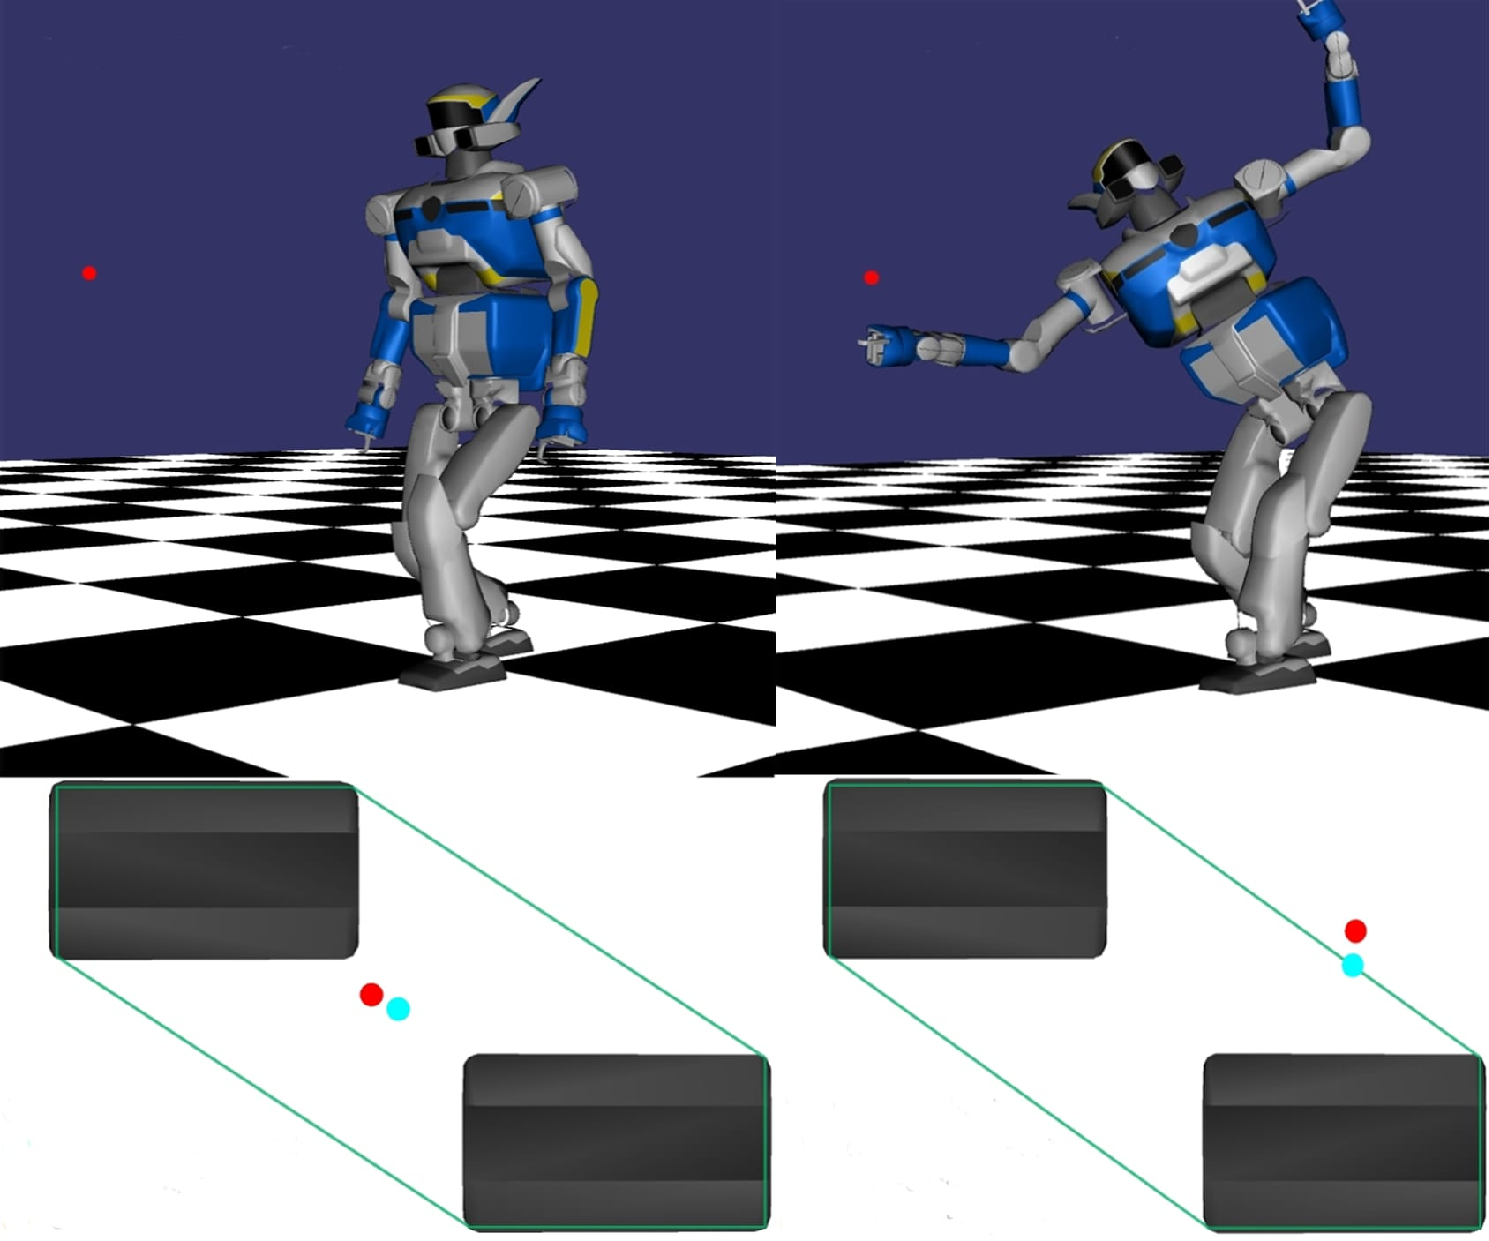
\includegraphics[scale=0.4]{rc_inertial_params/classic_merge.pdf}}\quad
\end{subfigure}
\begin{subfigure}
[Robust control illustrating the robot right end effector reaching close to the goal without losing balance]{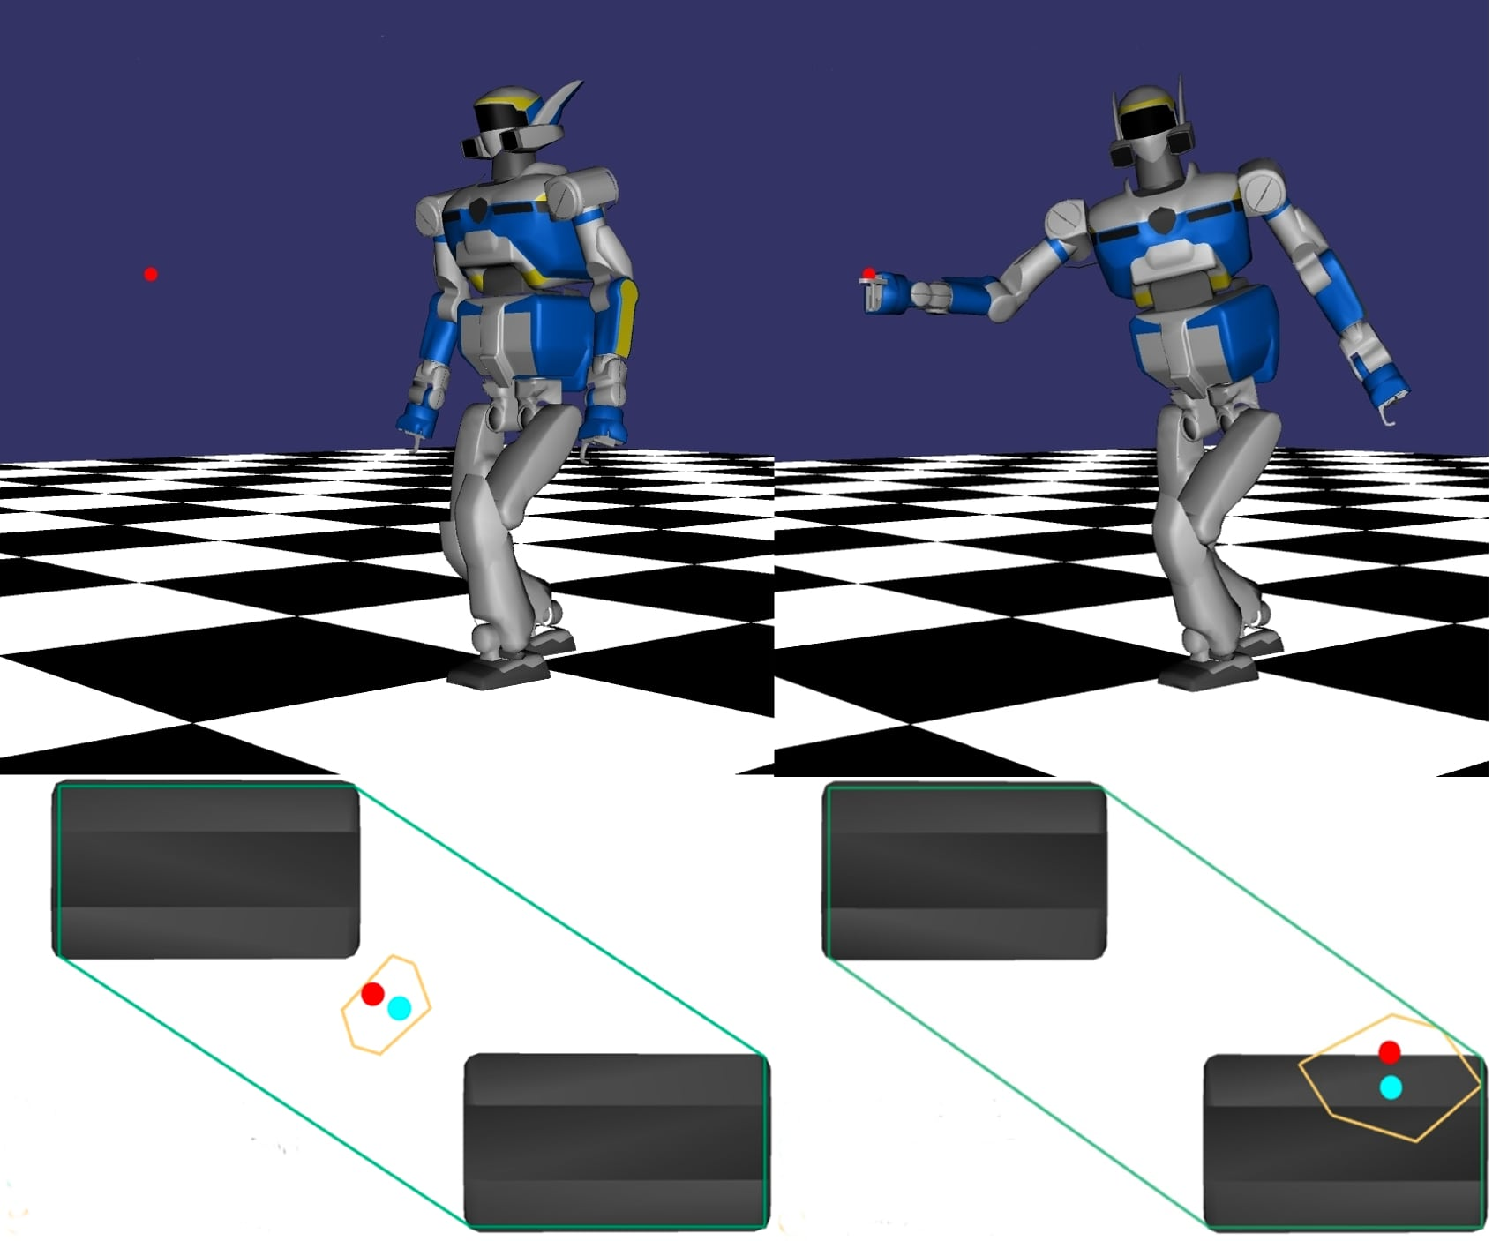
\includegraphics[scale=0.4]{rc_inertial_params/robust_merge.pdf}}\quad
\end{subfigure}\\
 \tikzcircle{3pt}  \footnotesize Real Capture Point \tikzcircle[turquoise, fill=turquoise]{3pt} Estimated Capture Point   \tikzcircle[green, fill=green]{3pt} Support Polygon   \tikzcircle[yellow, fill=yellow]{3pt} Capture Point Polytope

\caption{Screenshots of HRP-2 executing Test 1 to reach the ball target with the robust controller.}
\label{fig:control}
\end{figure*}


\begin{table*}[!tbph]
\begin{center}
\caption{Results of Test 1. For each controller we show the number of falls (Falls), the average time to complete the motion (Task Time) and the average distance of the end-effector to the target at the end of the motion (Task Error).}
\begin{tabular}{ |l|l|l|l|l|l|l|l| }
\hline
\multicolumn{2}{|c|}{Uncertainties}&\multicolumn{3}{|c|}{Classic Controller}&\multicolumn{3}{|c|}{Robust Controller}\\
\hline Max Mass & Max CoM &{Falls}& Task &{Task} & Falls & Task& Task  \\
Error & Error & & Time   &  Error & &  Time & Error\\ 
{[\%]} & [mm] & [\%]  &  [s]  &  [mm]  & [\%]  &  [s] & [mm]\\ 
\hline
% 10 & 12.5& 35& 6.22&4& 1& 5.26& 5\\
% 10 & 25  & 31 & 6.30&  5& 0& 7.32& 12\\
% 10 & 50  & 43 & 4.49 & 70 & 0 & 4.66 & 110\\
% 30 & 50  & 43 & 4.48 & 70 & 0 & 4.68 & 110\\
% 30 & 100 & 40 & 5.44 & 30 & 4 & 5.81 & 80 \\
10 & 10 & 31 & 4.4 & 49 & 3 & 4.5 & 60\\
10 & 20 & 33 & 4.3 & 52 & 1 & 4.5 & 69 \\
10 & 40 & 45 & 4.3 & 55 & 3 & 4.7 & 102\\ 
20 & 10 & 38 & 4.2 & 49 & 11 & 4.5 & 77\\
20 & 20 & 49 & 4.5 & 51 & 9 & 4.55 & 103 \\
20 & 40 & 45 & 4.5 & 59 & 14 & 4.72 & 122 \\
\hline
\end{tabular}
\label{tab:test1}
\end{center}
\end{table*}
\subsection{Test 1}
In this test we set the right end-effector target far in front of the robot.
Fig.~\ref{fig:control}  shows some screen shots of the simulations.
To reach the target the robot must move its CoM (and hence also its capture point) close to the boundaries of its support polygon. 
Table~\ref{tab:test1} presents the results. 
Regardless of the magnitude of the inertial parameter errors, the robust controller managed to prevent the robot from falling almost always, while with the  standard controller the robot fell more than 30\% of the times.
However, since the target was far away from the robot, the robust controller did not manage to reach it because that would have required violating the robust balance constraints.
\begin{table*}[!h]
\begin{center}
\caption{Results of Test 2. For each controller we show the number of falls (Falls), the average time to complete the motion (Task Time) and the average distance of the end-effector to the target at the end of the motion (Task Error).}
\begin{tabular}{ |l|l|l|l|l|l|l|l| }
\hline Max Mass & Max CoM &{Falls}& Task &{Task} & Falls & Task& Task  \\
Error & Error & & Time   &  Error & &  Time & Error\\ 
{[\%]} & [mm] & [\%]  &  [s]  &  [mm]  & [\%]  &  [s] & [mm]\\ 
\hline
% 10 & 12.5 & 59 & 3.64& 0 & 5 & 3.06& 0\\
% 10 & 25.0 & 42 & 3.40 & 0.18 & 4 & 2.94 & 0.12 \\
10 & 10 & 29 & 3.94 & 2 & 0 & 3.4 & 2 \\
10 & 20 & 35 & 3.4 & 2 & 2 & 3.0 & 2 \\
10 & 40 & 42 & 3.86 & 4 & 0 & 2.6 & 4 \\
20 & 10 & 43 & 3.6 & 3 & 0 & 2.8 & 4 \\
20 & 20 & 45 & 3.5 & 3 & 0 & 2.5 & 4 \\
20 & 40 & 45 & 3.0 & 5 & 0 & 2.1 & 5 \\

\hline
\end{tabular}
\label{tab:test2}
\end{center}
\end{table*}
\subsection{Test 2}
In this test we moved the right end-effector target closer to the robot, so that HRP-2 can reach it without moving its CoM close to the support polygon boundaries.
However, we increased the desired speed of reaching (by increasing the gains of the reaching task).
This affected the velocity of the CoM, which in turns affected the capture point, making it reach the boundaries of the support polygon.
The difference with respect to Test 1 is that in this case also the robust controller can reach the target.
Table~\ref{tab:test2} summarizes the results.

Similarly to Test 1, the classic controller leads the robot to a fall in more than 30\% of the cases.
However, contrary to Test 1, this time the robust controller also manages to reach the target, because it is located closer to the robot.
This test shows that being robust does not necessarily implies that we have to sacrifice performance.



%!TEX root =  ../root.tex
\section{Conclusions}
\label{sec:conclusions}
This chapter presented a novel optimization-based inverse-dynamics controller that can balance a legged robot despite bounded uncertainties in its inertial parameters. The controller is based on the state-or-the-art control framework Task-Space Inverse Dynamics. In particular, this work is based on the capture-point inequalities~\cite{Ramos2014a}, which can be included in the controller formulation to ensure the balance of the robot on a level ground. We extended these capture-point inequalities to be robust to bounded uncertainties in the inertial parameters of the robot. The resulting optimization problem is still a Quadratic Program with the same number of variables and inequalities. Moreover, the time required for the additional computation of the robust controller is negligible in this context (i.e. a few microseconds).

We tested the robust controller in simulations with the HRP-2 robot, trying to reach a target position with its right end-effector while balancing. We performed several batches of 100 simulations each, introducing different errors in the inertial parameters and varying the position of the target position and the required speed of motion. Comparisons against a classic TSID controller have shown impressive improvements in terms of fall prevention.

\subsection{Future Work}
In the derivation of the robust controller we saw that the inertial parameters appear in different terms of the optimization problem.
In this preliminary work we focused only on how the uncertainties affect the CoM position.
We believe it should be possible to extend this analysis to the other terms in the capture-point inequalities: CoM velocity, CoM altitude, CoM Jacobian and its time derivative. 
Extending it also to the mass matrix and the bias forces is an interesting future direction, but it seems more challenging because of nonlinearities.

Another issue of the presented approach is that it is rather conservative. As we saw in Test 1, this can lead to poor performance, which can be unacceptable on a real system. Modeling uncertainties with probability distributions (rather than with polytopes) may lead to a less conservative behavior of the system, and it is thus an interesting future direction. In our previous work~\cite{DelPrete2015b} we presented another robust controller, which was robust to joint-torque tracking errors.Integrating the two controllers together seems to be feasible and it would provide robustness to both kinds of uncertainties. In this preliminary work we focused on simulations to validate the controller formulation and to test it with different parameter errors. Of course, we plan also to test the generated movements on the real HRP-2 robot, to quantify how much it can benefit from this robustness.


\ifdefined\included
\else
\documentclass[a4paper,11pt,twoside]{StyleThese}
\usepackage{amsmath,amssymb}             % AMS Math
\usepackage[T1]{fontenc}
\usepackage[utf8x]{inputenc}
\usepackage{babel}
\usepackage{datetime}

\usepackage{lmodern}
\usepackage{tabularx}
%\usepackage{tabular}
\usepackage{multirow}

\usepackage{hhline}
\usepackage[left=1.5in,right=1.3in,top=1.1in,bottom=1.1in,includefoot,includehead,headheight=13.6pt]{geometry}
\renewcommand{\baselinestretch}{1.05}

% Table of contents for each chapter

\usepackage[nottoc, notlof, notlot]{tocbibind}
\usepackage{minitoc}
\setcounter{minitocdepth}{2}
\mtcindent=15pt
% Use \minitoc where to put a table of contents

\usepackage{aecompl}

% Glossary / list of abbreviations

\usepackage[intoc]{nomencl}
\iftoggle{ThesisInEnglish}{%
\renewcommand{\nomname}{Glossary}
}{ %
\renewcommand{\nomname}{Liste des Abréviations}
}

\makenomenclature

% My pdf code

\usepackage{ifpdf}

\ifpdf
  \usepackage[pdftex]{graphicx}
  \DeclareGraphicsExtensions{.jpg}
  \usepackage[a4paper,pagebackref,hyperindex=true]{hyperref}
  \usepackage{tikz}
  \usetikzlibrary{arrows,shapes,calc}
\else
  \usepackage{graphicx}
  \DeclareGraphicsExtensions{.ps,.eps}
  \usepackage[a4paper,dvipdfm,pagebackref,hyperindex=true]{hyperref}
\fi

\graphicspath{{.}{images/}}

%% nicer backref links. NOTE: The flag ThesisInEnglish is used to define the
% language in the back references. Read more about it in These.tex

\iftoggle{ThesisInEnglish}{%
\renewcommand*{\backref}[1]{}
\renewcommand*{\backrefalt}[4]{%
\ifcase #1 %
(Not cited.)%
\or
(Cited in page~#2.)%
\else
(Cited in pages~#2.)%
\fi}
\renewcommand*{\backrefsep}{, }
\renewcommand*{\backreftwosep}{ and~}
\renewcommand*{\backreflastsep}{ and~}
}{%
\renewcommand*{\backref}[1]{}
\renewcommand*{\backrefalt}[4]{%
\ifcase #1 %
(Non cité.)%
\or
(Cité en page~#2.)%
\else
(Cité en pages~#2.)%
\fi}
\renewcommand*{\backrefsep}{, }
\renewcommand*{\backreftwosep}{ et~}
\renewcommand*{\backreflastsep}{ et~}
}

% Links in pdf
\usepackage{color}
\definecolor{linkcol}{rgb}{0,0,0.4} 
\definecolor{citecol}{rgb}{0.5,0,0} 
\definecolor{linkcol}{rgb}{0,0,0} 
\definecolor{citecol}{rgb}{0,0,0}
% Change this to change the informations included in the pdf file

\hypersetup
{
bookmarksopen=true,
pdftitle="Évaluation de la sécurité des équipements grand public connectés à Internet",
pdfauthor="Yann BACHY", %auteur du document
pdfsubject="Thèse", %sujet du document
%pdftoolbar=false, %barre d'outils non visible
pdfmenubar=true, %barre de menu visible
pdfhighlight=/O, %effet d'un clic sur un lien hypertexte
colorlinks=true, %couleurs sur les liens hypertextes
pdfpagemode=None, %aucun mode de page
pdfpagelayout=SinglePage, %ouverture en simple page
pdffitwindow=true, %pages ouvertes entierement dans toute la fenetre
linkcolor=linkcol, %couleur des liens hypertextes internes
citecolor=citecol, %couleur des liens pour les citations
urlcolor=linkcol %couleur des liens pour les url
}

% definitions.
% -------------------

\setcounter{secnumdepth}{3}
\setcounter{tocdepth}{2}

% Some useful commands and shortcut for maths:  partial derivative and stuff

\newcommand{\pd}[2]{\frac{\partial #1}{\partial #2}}
\def\abs{\operatorname{abs}}
\def\argmax{\operatornamewithlimits{arg\,max}}
\def\argmin{\operatornamewithlimits{arg\,min}}
\def\diag{\operatorname{Diag}}
\newcommand{\eqRef}[1]{(\ref{#1})}

\usepackage{rotating}                    % Sideways of figures & tables
%\usepackage{bibunits}
%\usepackage[sectionbib]{chapterbib}          % Cross-reference package (Natural BiB)
%\usepackage{natbib}                  % Put References at the end of each chapter
                                         % Do not put 'sectionbib' option here.
                                         % Sectionbib option in 'natbib' will do.
\usepackage{fancyhdr}                    % Fancy Header and Footer

% \usepackage{txfonts}                     % Public Times New Roman text & math font
  
%%% Fancy Header %%%%%%%%%%%%%%%%%%%%%%%%%%%%%%%%%%%%%%%%%%%%%%%%%%%%%%%%%%%%%%%%%%
% Fancy Header Style Options

\pagestyle{fancy}                       % Sets fancy header and footer
\fancyfoot{}                            % Delete current footer settings

%\renewcommand{\chaptermark}[1]{         % Lower Case Chapter marker style
%  \markboth{\chaptername\ \thechapter.\ #1}}{}} %

%\renewcommand{\sectionmark}[1]{         % Lower case Section marker style
%  \markright{\thesection.\ #1}}         %

\fancyhead[LE,RO]{\bfseries\thepage}    % Page number (boldface) in left on even
% pages and right on odd pages
\fancyhead[RE]{\bfseries\nouppercase{\leftmark}}      % Chapter in the right on even pages
\fancyhead[LO]{\bfseries\nouppercase{\rightmark}}     % Section in the left on odd pages

\let\headruleORIG\headrule
\renewcommand{\headrule}{\color{black} \headruleORIG}
\renewcommand{\headrulewidth}{1.0pt}
\usepackage{colortbl}
\arrayrulecolor{black}

\fancypagestyle{plain}{
  \fancyhead{}
  \fancyfoot{}
  \renewcommand{\headrulewidth}{0pt}
}

%\usepackage{MyAlgorithm}
%\usepackage[noend]{MyAlgorithmic}
\usepackage[ED=MITT - STICRT, Ets=INSA]{tlsflyleaf}
%%% Clear Header %%%%%%%%%%%%%%%%%%%%%%%%%%%%%%%%%%%%%%%%%%%%%%%%%%%%%%%%%%%%%%%%%%
% Clear Header Style on the Last Empty Odd pages
\makeatletter

\def\cleardoublepage{\clearpage\if@twoside \ifodd\c@page\else%
  \hbox{}%
  \thispagestyle{empty}%              % Empty header styles
  \newpage%
  \if@twocolumn\hbox{}\newpage\fi\fi\fi}

\makeatother
 
%%%%%%%%%%%%%%%%%%%%%%%%%%%%%%%%%%%%%%%%%%%%%%%%%%%%%%%%%%%%%%%%%%%%%%%%%%%%%%% 
% Prints your review date and 'Draft Version' (From Josullvn, CS, CMU)
\newcommand{\reviewtimetoday}[2]{\special{!userdict begin
    /bop-hook{gsave 20 710 translate 45 rotate 0.8 setgray
      /Times-Roman findfont 12 scalefont setfont 0 0   moveto (#1) show
      0 -12 moveto (#2) show grestore}def end}}
% You can turn on or off this option.
% \reviewtimetoday{\today}{Draft Version}
%%%%%%%%%%%%%%%%%%%%%%%%%%%%%%%%%%%%%%%%%%%%%%%%%%%%%%%%%%%%%%%%%%%%%%%%%%%%%%% 

\newenvironment{maxime}[1]
{
\vspace*{0cm}
\hfill
\begin{minipage}{0.5\textwidth}%
%\rule[0.5ex]{\textwidth}{0.1mm}\\%
\hrulefill $\:$ {\bf #1}\\
%\vspace*{-0.25cm}
\it 
}%
{%

\hrulefill
\vspace*{0.5cm}%
\end{minipage}
}

\let\minitocORIG\minitoc
\renewcommand{\minitoc}{\minitocORIG \vspace{1.5em}}

\usepackage{multirow}
%\usepackage{slashbox}

\newenvironment{bulletList}%
{ \begin{list}%
	{$\bullet$}%
	{\setlength{\labelwidth}{25pt}%
	 \setlength{\leftmargin}{30pt}%
	 \setlength{\itemsep}{\parsep}}}%
{ \end{list} }

\newtheorem{definition}{Définition}
\renewcommand{\epsilon}{\varepsilon}

% centered page environment

\newenvironment{vcenterpage}
{\newpage\vspace*{\fill}\thispagestyle{empty}\renewcommand{\headrulewidth}{0pt}}
{\vspace*{\fill}}

\usepackage{tablefootnote}

\usepackage{hyperref}
\hypersetup{
     colorlinks   = true,
     citecolor    = violet
}
\usepackage{graphicx} % for pdf, bitmapped graphics files
\usepackage{amsmath} % assumes amsmath package installed
\usepackage{amssymb}  % assumes amsmath package installed
\usepackage{bm} % for using bold lowercase greek letters
\usepackage{array}
\usepackage{colortbl}	% to color table background
%\usepackage[table]{xcolor}
\usepackage{subfigure}  
\usepackage{tikz}
\newcommand{\tikzcircle}[2][red,fill=red]{\tikz[baseline=-0.5ex]\draw[#1,radius=#2] (0,0) circle ;}%
\definecolor{turquoise}{rgb}{0.28 1 0.92}
\newcommand{\fratop}[2]{\genfrac{}{}{0pt}{}{#1}{#2}}
\newcommand{\mx}[1]{\mathbf{\bm{#1}}} 				% Matrix symbol
\newcommand{\vc}[1]{\mathbf{\bm{#1}}} 					% Vector symbol
\newcommand{\degree}{\ensuremath{^\circ}}				% define the degree symbol
\newcommand{\pder}[2]{\frac{\partial#1}{\partial#2}}		% partial derivative
\newcommand{\ppder}[2]{\frac{\partial^2 #1}{\partial#2^2}}		% second partial derivative
\newcommand{\refframe}[1]{\mbox{\textless#1\textgreater}}	% to denote a reference frame
%\DeclareMathOperator*{\lexmin}{\text{lex}\!\min}			% lexmin
\DeclareMathOperator*{\minimize}{minimize}				% minimize
\DeclareMathOperator*{\maximize}{maximize}				% maximize
%\DeclareMathOperator*{\argmin}{\arg\!\min}				% argmin
%\DeclareMathOperator*{\argmax}{\arg\!\max}				% argmax
\DeclareMathOperator*{\st}{subject\,to}					% subject to
\DeclareMathOperator*{\dif}{\mathrm{d}}					% d
\DeclareMathOperator*{\half}{\frac{1}{2}}					% one half
\newcommand{\mat}[1]{\ensuremath{\begin{bmatrix}#1\end{bmatrix}}}	% matrix
\newcommand{\rank}[1]{\text{rank}(#1)}							% rank
%\newcommand{\diag}[1]{\text{diag}(#1)}							% diag
\newcommand{\x}{\ensuremath{\times}}
\newcommand{\spac}{\ensuremath{\quad}}						% alias for space in math environment
\newcommand{\dt}[0]{\ensuremath{\Delta t}}					% dt
\newcommand{\dx}[0]{\ensuremath{\delta x}}					% dx
\newcommand{\du}[0]{\ensuremath{\delta u}}					% du
\newcommand{\dhu}[0]{\ensuremath{\delta \hat{u}}}					% \hat{du}
\newcommand{\dbu}[0]{\ensuremath{\delta \bar{u}}}					% \bar{du}
\newcommand{\dtu}[0]{\ensuremath{\delta \tilde{u}}}					% \tilde{du}
\newcommand{\dhx}[0]{\ensuremath{\delta \hat{x}}}					% \hat{dx}
\newcommand{\DX}[0]{\ensuremath{\Delta X}}						% DX
\newcommand{\DU}[0]{\ensuremath{\Delta U}}						% DU
\newcommand{\Ts}[0]{\ensuremath{\top}}							% transpose symbol
\newcommand{\pinv}[0]{\ensuremath{\dagger}}					% pseudoinverse symbol
\newcommand{\Rv}[1]{\ensuremath{\mathbb{R}^{#1}}}				% set of real-valued vectors
\newcommand{\Rm}[2]{\ensuremath{\mathbb{R}^{#1\times #2}}}		% set of real-valued matrices
\newcommand{\Spd}[1]{\ensuremath{\mathbb{S}_+^{#1}}}			% set of symmetric positive-definite matrices
\newcommand{\card}[1]{\ensuremath{\left\vert{#1}\right\vert}}			% cardinality of a set
\DeclareMathOperator{\Tr}{Tr}							% trace
\newcommand{\Expect}{{\rm I\kern-.3em E}}				% expectation
\newcommand{\Normal}{\mathcal{N}}					% normal distribution
\newcommand{\Prob}[1]{\text{P}(#1)}						% probability
\newcommand{\vech}[1]{\text{vech}(#1)}						% vech

\newcommand{\sethree}{\ensuremath{SE(3)}}
\newcommand{\CS}{$\mathcal{CS}$}
\newcommand{\WS}{$\mathcal{WS}$}
\newcommand{\CSfree}{$\mathcal{CS}_{free}$}
\newcommand{\CSobst}{$\mathcal{CS}_{obst}$}
\newcommand{\M}[0]{$\mathcal{M}$}

%\algnewcommand{\algorithmicgoto}{\textbf{go to}}%
%%\algnewcommand{\Goto}[1]{\algorithmicgoto~\ref{#1}}%
%\algnewcommand{\Goto}{\algorithmicgoto\xspace}%
%\algnewcommand{\Label}{\State\unskip}

\newenvironment{definition}[1][Definition]{\begin{trivlist}
\item[\hskip \labelsep {\bfseries #1}]}{\end{trivlist}}

\usepackage{epstopdf}
\usepackage[colorinlistoftodos,prependcaption,textsize=tiny]{todonotes}
\newcommand\explainmore[1]{\textcolor{red}{#1}}
\newcommand\refrephrase[1]{\textcolor{yellow}{#1}}
\newcommand\donerephrasing[1]{\textcolor{green}{#1}}

%DIF PREAMBLE EXTENSION ADDED BY LATEXDIFF
%DIF UNDERLINE PREAMBLE %DIF PREAMBLE
\RequirePackage[normalem]{ulem} %DIF PREAMBLE
\RequirePackage{color}\definecolor{RED}{rgb}{1,0,0}\definecolor{BLUE}{rgb}{0,0,1} %DIF PREAMBLE
\providecommand{\DIFadd}[1]{{\protect\color{blue}\uwave{#1}}} %DIF PREAMBLE
\providecommand{\DIFdel}[1]{{\protect\color{red}\sout{#1}}}                      %DIF PREAMBLE
%DIF SAFE PREAMBLE %DIF PREAMBLE
\providecommand{\DIFaddbegin}{} %DIF PREAMBLE
\providecommand{\DIFaddend}{} %DIF PREAMBLE
\providecommand{\DIFdelbegin}{} %DIF PREAMBLE
\providecommand{\DIFdelend}{} %DIF PREAMBLE
%DIF FLOATSAFE PREAMBLE %DIF PREAMBLE
\providecommand{\DIFaddFL}[1]{\DIFadd{#1}} %DIF PREAMBLE
\providecommand{\DIFdelFL}[1]{\DIFdel{#1}} %DIF PREAMBLE
\providecommand{\DIFaddbeginFL}{} %DIF PREAMBLE
\providecommand{\DIFaddendFL}{} %DIF PREAMBLE
\providecommand{\DIFdelbeginFL}{} %DIF PREAMBLE
\providecommand{\DIFdelendFL}{} %DIF PREAMBLE
%DIF END PREAMBLE EXTENSION ADDED BY LATEXDIFF


\begin{document}


\sloppy
\begin{document}
\fi


\chapter*{Conclusion}
\addstarredchapter{Conclusion} %Sinon cela n'apparait pas dans la table des matières

\ifdefined\included
\else
\bibliographystyle{acm}
\bibliography{These}
\end{document}
\fi
% \appendix
% \chapter{Exemple d'annexe}
\label{chap:annexe1}

\section{Exemple d'annexe}


\bibliographystyle{StyleThese}
%\bibliographystyle{plain}
\bibliography{These}

% \cleardoublepage
% \begin{vcenterpage}
% \noindent\rule[2pt]{\textwidth}{0.5pt}
% \\
% \iftoggle{ThesisInEnglish}{%
% {\large\textbf{Abstract:}}
% }{%
% {\large\textbf{Résumé :}}
% }
% resume
% \iftoggle{ThesisInEnglish}{%
% {\large\textbf{Keywords:}}
% }{%
% {\large\textbf{Mots clés :}}
% }
% mots, clefs
% \\
% \noindent\rule[2pt]{\textwidth}{0.5pt}
% \end{vcenterpage}

\end{document}
